\chapter{Livello di rete}

Il livello rete nello stack TCP/IP è responsabile della consegna dei datagrammi tra gli host.\
Questo procedimento comprende numerosi aspetti, come ad esempio la progettazione degli indirizzi logici necessari per identificare in maniera univoca gli host connessi ad Internet.\
I\
oltre, richiede anche degli opportuni protocolli di instradamento che permettano ai pacchetti del livello di rete di giungere dalla sorgente fino alla destinazione.

\section{Introduzione}

\begin{figure}[H]
    \centering
    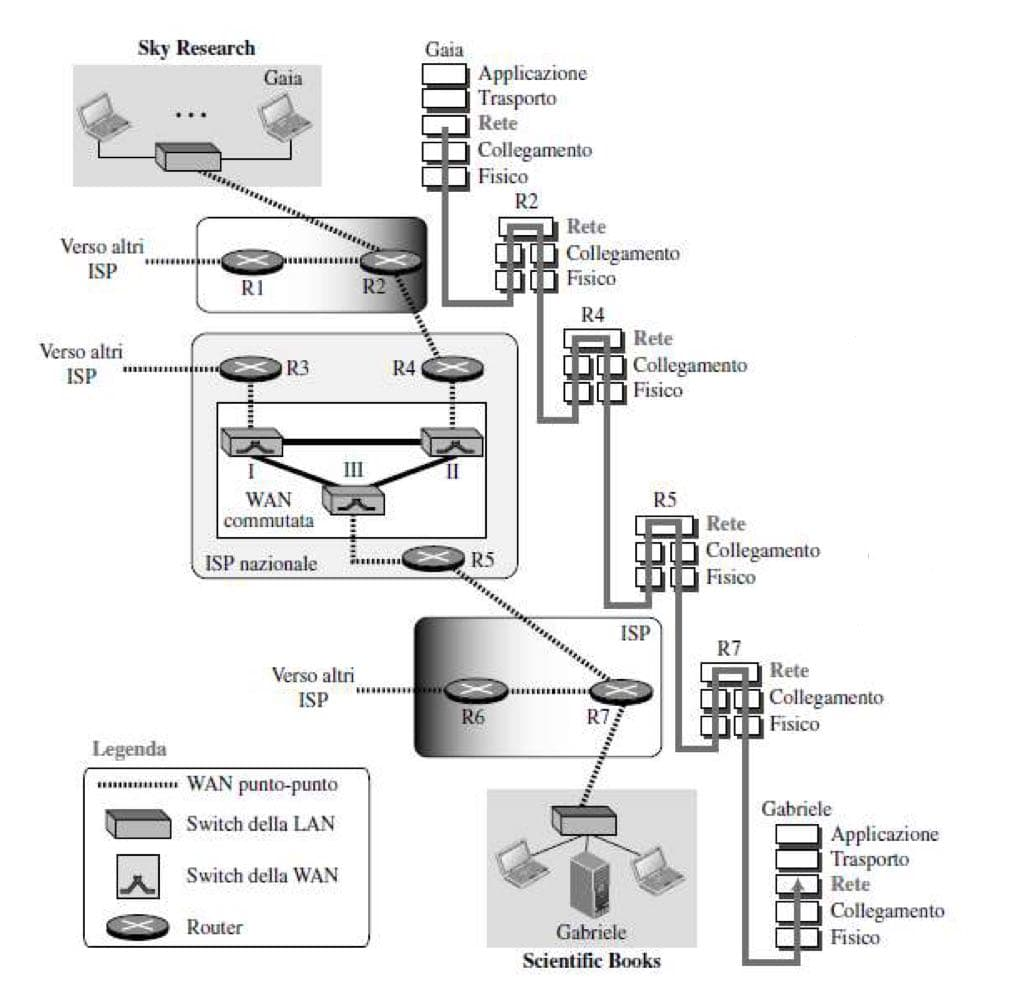
\includegraphics[width = 0.8\textwidth]{immagini/Livello_Rete.jpg}
    \caption{Comunicazione a livello rete}
    \label{fig}
\end{figure}

\noindent La Figura \ref{fig} mostra la comunicazione tra Gaia e Gabriele a livello di rete.\
La figura mostra come Internet sia formata da molte reti (o collegamenti) connessi tramite opportuni dispositivi.\
In altre parole Internet è un'internetwork (una rete di reti), cioè una combinazione di LAN e WAN.\
Per comprendere meglio il ruolo del livello di rete (o del livello di internetwork), dobbiamo considerare i dispositivi di interconnessione (router o switch) che connettono tra loro LAN e WAN.

Come mostra la figura, il livello di rete è presente nell'host sorgente, nell'host destinatario e in tutti i router lungo il percorso (R2, R4, R5 e R7).\
Nell'host sorgente (Gaia), il livello di rete accetta un pacchetto (più precisamente un segmento o un datagramma utente) dal livello trasporto, incapsula il pacchetto in un datagramma del livello rete e lo consegna al livello di collegamento.\
Nell'host di destinazione (Gabriele), il datagramma viene decapsulato, il pacchetto viene estratto e consegnato al livello trasporto.\
Sebbene gli host sorgente e destinazione siano coinvolti in tutti e cinque i livelli della pila di protocolli TCP/IP, i router utilizzano solamente tre livelli durante l'attività vera e propria di instradamento dei pacchetti.\
Tuttavia i router possono aver bisogno dei livelli di trasporto ed applicazione per alcuni scopi particolari (ad esempio per coordinarsi con altri router).\
Un router presente lungo il percorso tra sorgente e destinazione normalmente viene rappresentato con almeno due livelli di collegamento e due livelli fisici, in quanto riceve un pacchetto da una rete e lo invia su un'altra rete.

\subsection{Servizi a livello di rete}

\subsubsection{\emph{Suddivisione in pacchetti}}

Il primo compito del livello di rete è sicuramente la suddivisione dei dati in pacchetti (packetizing):\ alla sorgente incapsulare i dati ricevuti dal livello superiore (payload) in un pacchetto (detto anche datagramma) del livello di rete e, viceversa, alla destinazione decapsulare il payload del pacchetto.\
In altre parole, uno dei compiti del livello di rete è quello di portare un payload dalla sorgente alla destinazione senza modificarlo o utilizzarlo.\
Il livello di rete funge quindi solamente da vettore, proprio come un ufficio postale, che è responsabile della consegna dei pacchi da un mittente a un ricevente senza modificare o utilizzare il loro contenuto.

L'host sorgente riceve il payload da un protocollo di livello superiore, aggiunge un'intestazione (header) che contiene gli indirizzi sorgente e destinazione oltre ad alcune altre informazioni richieste dal protocollo del livello di rete e consegna il pacchetto al livello di collegamento.\
La sorgente non è autorizzata a modificare il payload a meno che esso non sia troppo grande per il trasferimento e quindi necessiti di essere suddiviso in frammenti più piccoli (frammentazione).

L'host di destinazione riceve il pacchetto di livello rete dal suo livello di collegamento, lo apre e consegna il payload al protocollo di livello superiore corrispondente.\
Se il pacchetto è stato frammentato alla sorgente o nei router lungo il percorso, il livello di rete deve attendere l'arrivo di tutti i frammenti di quel pacchetto, riassembrarli e solo a questo punto consegnare il payload al protocollo di livello superiore.

I router lungo il percorso non sono autorizzati ad aprire i pacchetti che hanno ricevuto a meno che tali pacchetti non debbano essere frammentati.\
Inoltre, i router non possono nemmeno modificare gli indirizzi sorgente e destinazione.\
Essi verificano semplicemente gli indirizzi allo scopo di inoltrare il pacchetto alla rete successiva lungo il percorso.\
Tuttavia, se un pacchetto deve essere frammentato, l'intestazione sarà copiata in tutti i frammenti ma saranno anche necessari alcuni cambiamenti.

\subsubsection{\emph{Instradamento (routing)}}

Un altro compito del livello di rete, tanto importante quanto il primo, è l'instradamento (routing).\
Il compito del livello di rete è quello di instradare il pacchetto dalla sua sorgente alla destinazione.\
Una rete fisica non è altro che la combinazione di varie reti (LAN e WAN) e dei router che le collegano.\
Ciò significa che, normalmente, c'è più di un percorso che va dalla sorgente alla destinazione.\
Il livello di rete deve trovare il \emph{migliore} tra tali possibili percorsi.\
La scelta del percorso migliore deve avvenire per mezzo di opportune strategie.\
Nella Internet di oggi questo avviene tramite l'esecuzione di alcuni \emph{protocolli di routing} (\emph{protocolli di instradamento}), che hanno lo scopo di aiutare i router a condividere e coordinare la loro conoscenza sulla rete.\
Il risultato è la creazione di tabelle di instradamento che verranno utilizzate per decidere come instradare i pacchetti al momento del loro arrivo nei router.\
I protocolli d'instradamento, di cui parleremo successivamente in questo capitolo, devono essere eseguiti prima che qualsiasi altra comunicazione possa avvenire.

\subsubsection{\emph{Inoltro (forwarding)}}

Se routing significa applicare strategie ed eseguire protocolli per creare tabelle di instradamento in ogni router, l'inoltro (\emph{forwarding}) si può definire come l'azione eseguita dai router quando un pacchetto arriva ad una delle sue interfacce.\
La tabella d'inoltro (\emph{forwarding table}) che viene normalmente utilizzata da un router per completare tale azione viene talvolta definita, in modo piuttosto ambiguo, routing table.\
Quando un router riceve un pacchetto da una delle reti a cui è collegato direttamente, deve inoltrare il pacchetto ad un'altra delle reti a cui è collegato (nell'instradamento unicast) o a più reti a cui è collegato (nel caso di instradamento multicast).\
Per prendere questa decisione il router utilizza alcune informazioni che si trovano nell'intestazione del pacchetto, ovvero l'indirizzo di destinazione o un'etichetta, per trovare la giusta interfaccia di output all'interno della tabella d'inoltro.

\begin{figure}[H]
    \centering
    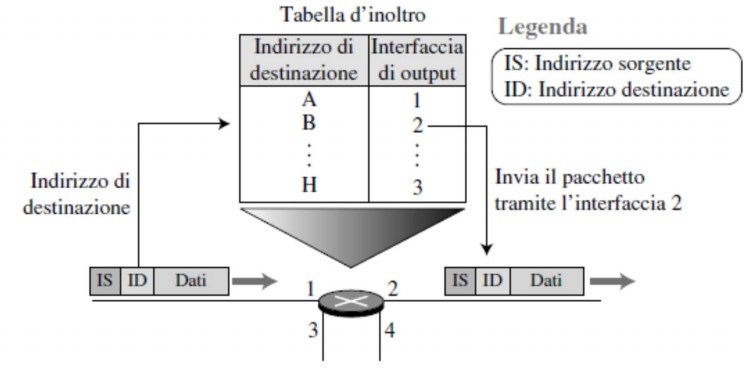
\includegraphics[width = 0.8\textwidth]{immagini/Forwarding.jpg}
\end{figure}

\subsubsection{\emph{Controllo degli errori}}

Sebbene il controllo degli errori possa essere realizzato anche a livello di rete, i progettisti di tale livello in Internet hanno deciso di ignorare questo aspetto.\
Una delle ragioni di tale decisione è il fatto che i pacchetti a livello di rete possono essere frammentati in ciascun router, un fatto che renderebbe il controllo degli errori piuttosto inefficiente visto che dovrebbe lavorare su dati parziali.

I progettisti del livello rete, tuttavia, hanno aggiunto un campo denominato checksum nel pacchetto, al fine di controllare eventuale errori presenti sull'intestazione, ma non c'è alcuna verifica per quanto riguarda il payload.\
Questa checksum può rilevare cambiamenti o errori nell'intestazione del pacchetto che avvengono durante il trasferimento tra coppie di dispositivi o tra la sorgente e la destinazione.

Dobbiamo aggiungere che, nonostante il livello di rete in Internet non fornisca direttamente il controllo degli errori, Internet utilizza un protocollo ausiliario (chiamato ICMP) che fornisce una sorta di controllo degli errori nel caso un pacchetto venga scartato o contenga informazioni sconosciute nell'intestazione.

\section{Protocolli di livello rete}

In questa sezione si vedrà come il livello di rete è implementato nella pila di protocolli TCP/IP.\
Nel corso del tempo i protocolli di livello rete hanno avuto molte versioni differenti.\
In questa sezione si vedrà la versione attuale (4), mentre nell'ultima parte del capitolo sarà brevemente trattata la nuova versione (6), che è all'orizzonte, ma ancora scarsamente utilizzata.

Nella versione 4 il livello di rete può essere visto come formato da un protocollo principale e da tre protocolli ausiliari.\
Il protocollo principale, l'Internet Protocol versione 4 (IPv4) è responsabile della suddivisione in pacchetti, dell'inoltro (forwarding) e della consegna (delivery) dei datagrammi a livello di rete.\
L'Internet Control Message Protocol versione 4 (ICMPv4) aiuta l'IPv4 a gestire alcuni errori che possono avvenire nella consegna a livello di rete.\
L'Internet Group Management Protocol (IGMP) viene utilizzato per supportare l'IPv4 nella gestione del multicasting.\
Infine, l'Address Resolution Protocol (ARP) viene usato per far interagire il livello di rete e quello di collegamento.\
Più in dettaglio, ARP ha il compito specifico di permettere l'associazione tra indirizzi di livello rete e indirizzi di livello di collegamento.

L'IPv4 è un protocollo inaffidabile e senza connessione, basato su datagrammi.\
IPv4 offre un servizio di consegna di tipo best-effort, ovvero il protocollo fa del suo meglio per consegnare i dati che sono stati spediti ma non offre alcuna garanzia.\
Con il termine \emph{best-effort} si intende che i datagrammi IPv4 possono essere danneggiati, persi, arrivare fuori ordine o in ritardo e possono anche generare congestione nella rete.\
Se è importante l'affidabilità allora è necessario associare ad IPv4 un protocollo di livello trasporto che sia in grado di garantirla aggiungendo alcune funzionalità, come ad esempio il TCP.\

Come detto in precedenza, l'IPv4 è un protocollo senza connessione per reti a commutazione di pacchetto che utilizza un approccio basato su datagrammi.\
Questo significa che ogni datagramma viene gestito in modo del tutto indipendente e quindi può seguire un percorso diverso tra l'origine e la destinazione.\
Ciò implica che i datagrammi inviati dalla stessa sorgente alla stessa destinazione potrebbero arrivare fuori ordine.\
Inoltre alcuni potrebbero andare persi o essere danneggiati durante la trasmissione.\
Anche in questo caso IPv4 deve far affidamento su un protocollo di livello superiore (per esempio, il livello trasporto) per risolvere questi problemi.

\subsection{Formato di datagrammi IPv4}

\begin{figure}[H]
    \centering
    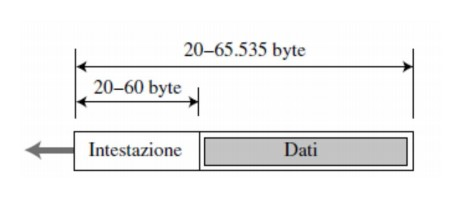
\includegraphics[width=0.5\textwidth]{immagini/Datagramma.jpg}
    \caption*{Datagramma IP}
\end{figure}

I pacchetti usati dal protocollo IP vengono definiti \emph{datagrammi} IP.\
Un datagramma è un pacchetto di lunghezza variabile composto da due parti:\ un'intestazione (header) e un campo dati (payload).\
L'intestazione è lunga da 20 a 60 byte e contiene le informazioni essenziali per il routing e la consegna dei datagrammi.\
Per comodità di lettura normalmente si rappresenta l'intestazione TCP/IP sotto forma di righe di 4 byte (32 bit) ciascuna.

\begin{figure}[H]
    \centering
    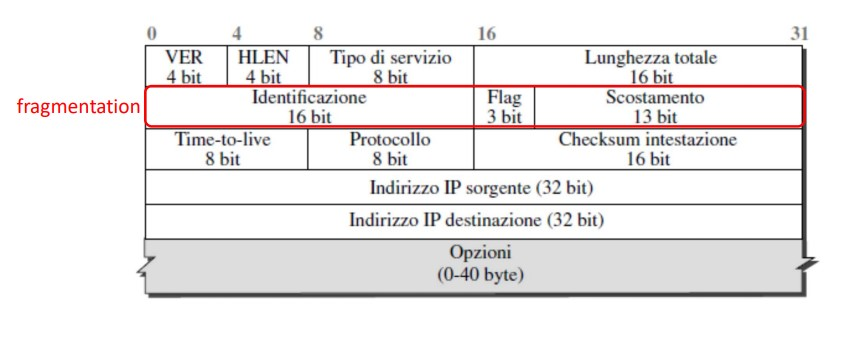
\includegraphics[width = 0.8\textwidth]{immagini/Intestazione_datagramma.jpg}
    \caption*{Formato dell'intestazione}
\end{figure}

\begin{itemize}
    \item \textbf{\emph{Numero versione}}.\
          Questo campo (VER), formato da 4 bit, definisce la versione del protocollo IP.\
          Visto che si sta trattando IPv4 ovviamente il valore sarà 4.
    \item \textbf{\emph{Lunghezza dell'intestazione}}.\
          Il campo lunghezza intestazione (H\-LEN), formato da 4 bit, definisce la lunghezza totale dell'intestazione del datagramma in parole formato da 4 byte.\
          Il datagramma IPv4 ha un'intestazione di lunghezza variabile.\
          Quando un dispositivo riceve un datagramma deve sapere dove finisce l'intestazione e dove iniziano i dati incapsulati nel datagramma.\
          La lunghezza dell'intestazione, come numero di byte, deve essere rappresentata facendo uso dei soli 4 bit che formano questo campo.\
          Per questo motivo, si ricorre ad una rappresentazione sotto forma di parole da 4 byte.\
          Questo significa che la lunghezza totale dell'intestazione viene divisa per 4 e il valore inserito nel campo.\
          Il ricevente ovviamente deve moltiplicare il valore di questo campo per 4 per trovare l'effettiva lunghezza totale.
    \item \textbf{\emph{Tipo servizio}}.\
          Secondo la progettazione originaria dell'intestazione IP, questo campo doveva specificare il tipo di servizio, ovvero il modo in cui il datagramma doveva essere gestito dai router lungo il percorso.\
          Alla fine degli anni '90, l'IETF ha ridefinito il campo per fornire i cosiddetti \emph{servizi differenziati}.
    \item \textbf{\emph{Time-to-live (TTl, tempo di vita)}}.\
          A causa di alcuni malfuzionamenti dei protocolli di instradamento (che si vedranno in seguito), può accadere che un datagramma circoli su Internet, visitando alcune reti più di una volta, ma senza raggiungere la destinazione finale.\
          Ovviamente questo porta alla creazione di traffico del tutto inutile.\
          Il campo TTL viene usato per controllare il numero massimo di salti (hop), cioè il numero di router visitati dal datagramma.\
          Quando un host sorgente invia il datagramma, esso memorizza un valore iniziale in questo campo.\
          Questo valore è approssimativamente pari a due volte il numero massimo di salti tra due host qualsiasi presenti su Internet.\
          Ogni router che elabora il datagramma decrementa di un'unità questo numero.\
          Se il TTL, dopo essere stato diminuito, giunge a zero allora il router scarta il datagramma.
    \item \textbf{\emph{Lunghezza totale}}.\
          Questo campo, da 16 bit, definisce la lunghezza totale (intestazione più dati), espressa in byte, del datagramma IP.\
          Un campo di 16 bit può rappresentare una lunghezza massima di 65.535 byte (nel caso in cui tutti i bit siano impostati a 1).\
          Tuttavia la dimensione dei datagrammi normalmente è molto inferiore a questo massimo.\
          Questo campo è utile al dispositivo ricevente per determinare se il pacchetto in ricezione è arrivato completamente.
    \item \textbf{\emph{Identificazione, flag e scostamento di frammentazione (offset)}}.\
          Questi tre campi riguardano la frammentazione dei datagrammi IP che avviene quando la loro dimensione è maggiore rispetto a quella che la tecnologia di livello collegamento sottostante è in grado di trasportare.
    \item \textbf{\emph{Protocollo}}.\
          In TCP/IP, la sezione relativa ai dati di un pacchetto, chiamata \emph{payload}, incapsula l'intero pacchetto di un altro protocollo (solitamente di livello superiore).\
          Un datagramma, per esempio, può portare un pacchetto che appartiene a un protocollo di livello trasporto come UDP (quindi un datagramma utente) o TCP (quindi un segmento).\
          Un datagramma può anche portare un pacchetto di un altro protocollo che usa direttamente il servizio offerto da IP, come ad esempio alcuni protocolli di instradamento o alcuni protocolli ausiliari.\
          Gli enti di gestione Internet hanno assegnato ad ogni protocollo che fa uso del servizio IP un numero univoco composto da 8 bit, numero che viene di volta in volta inserito nel campo protocollo all'interno dell'intestazione.\
          Quando il payload viene incapsulato in un datagramma nella sorgente, il numero di protocollo corrispondente viene inserito in questo campo; quando il datagramma arriva a destinazione, il valore di questo campo permette di definire a quale protocollo va consegnato il payload estratto dal datagramma.\
          In altre parole, questo campo fornisce il multiplexing alla sorgente e il demultiplexing a destinazione.\
          È bene notare che il campo protocollo a livello di rete ha un ruolo simile ai numeri di porta a livello trasporto.
          \begin{figure}[H]
              \centering
              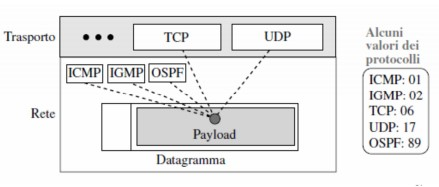
\includegraphics[width = 0.6\textwidth]{immagini/Multiplexing_Demultiplexing.jpg}
              \caption*{Multiplexing e demultiplexing utilizzando il valore del campo protocollo}
          \end{figure}

    \item \textbf{\emph{Checksum dell'intestazione}}.\
          IP è un protocollo non affidabile, ad esempio non controlla se i dati incapsulati in un datagramma vengono danneggiati durante la trasmissione.\
          IP lascia l'onere del controllo degli errori nei dati trasmessi al protocollo che è proprietario del payload, come ad esempio UDP o TCP.\
          L'intestazione del datagramma, tuttavia, viene aggiunta dall'IP e il controllo degli errori è quindi una sua responsabilità.\
          Gli errori nell'intestazione IP possono essere un grosso problema.\
          Se l'indirizzo IP di destinazione è danneggiato, il pacchetto sarà consegnato all'host sbagliato.\
          Se il campo protocollo è danneggiato, il payload sarà consegnato al protocollo errato.\
          Se i campi relativi alla frammentazione sono danneggiati, il datagramma non sarà riassemblato correttamente a destinazione, e così via.\
          Per tali ragioni IP aggiunge un campo checksum che riguarda la sola intestazione ma non il payload.\
          È bene ricordare che, siccome il valore di alcuni campi, come TTL, la frammentazione e le opzioni, possono cambiare da router a router, il checksum deve essere ricalcolato in ogni router.\
          Il checksum, che viene inserito in un campo da 16 bit, è ottenuto come il complemento della somma degli altri campi dell'intestazione, il tutto utilizzando l'aritmetica complemento a uno.
    \item \textbf{\emph{Indirizzi sorgente e destinazione}}.\
          Questi campi, lunghi 32 bit, definiscono rispettivamente l'indirizzo IP della sorgente e quello della destinazione.\
          L'host sorgente dovrebbe conoscere a priori il suo indirizzo IP.\
          L'indirizzo IP di destinazione invece è noto al protocollo che utilizza il servizio offerto da IP oppure viene ottenuto per mezzo del DNS.\
          Da notare che il valore di questi campi deve rimanere immutato durante tutto il tragitto del datagramma IP dell'host sorgente a quello di destinazione.
    \item \textbf{\emph{Opzioni}}.\
          L'intestazione di un datagramma può avere fino a 40 byte di opzioni.\
          Le opzioni possono essere usate per il test o il debug della rete.
    \item \textbf{\emph{Payload (dati)}}.\
          I dati trasportati ovviamente sono la ragione principale per la creazione del datagramma.\
          Il payload è il pacchetto che deriva dagli altri protocolli che usano il servizio dell'IP, siano questi di livello superiore (per esempio, TCP o UDP) o di pari livello (per esempio, ICMP) nello stack TCP/IP.
\end{itemize}

\subsubsection{\emph{Frammentazione}}

Per giungere alla destinazione, un datagramma IP può dover viaggiare attraverso varie reti, ognuna con caratteristiche differenti.\
Ogni router toglie il datagramma dal frame di livello collegamento che ha ricevuto, lo elabora e poi lo incapsula in un nuovo frame.\
Il formato e la dimensione del frame ricevuto dipendono dalla tecnologia fisica e da quella di livello di collegamento utilizzati per trasportare il frame.\
Viceversa, il formato e la dimensione del frame inviato dipendono dalla tecnologia fisica e da quella di livello di collegamento della rete su cui il frame verrà inviato.\
Per esempio se un router collega una LAN a una WAN, riceverà un frame in formato LAN e invierà un nuovo frame in formato WAN.

\paragraph{\emph{Maximum Transfer Unit (MTU)}} Ogni protocollo di livello collegamento ha il proprio formato di frame.\
Una delle caratteristiche di ciascun formato è la dimensione massima del payload che può essere incapsulato nel frame.\
In altre parole, quando un datagramma è racchiuso in un frame, la dimensione totale del datagramma deve essere inferiore rispetto a questa misura massima, che è definita dalle restrizioni imposte dall'hardware e dal software usati nella rete.

Per rendere il protocollo IP indipendente dai livelli sottostanti, i progettisti hanno deciso di fissare la lunghezza massima del datagramma IP a 65.535 byte.\
Questo rende la trasmissione efficiente nel caso si usi un protocollo di livello collegamento con una MTU di tali dimensioni.\
Tuttavia, altre tecnologie di rete richiedono che il datagramma sia suddiviso in parti più piccole per poter essere trasportato.\
Questo procedimento viene chiamato \emph{frammentazione}.

\begin{figure}[H]
    \centering
    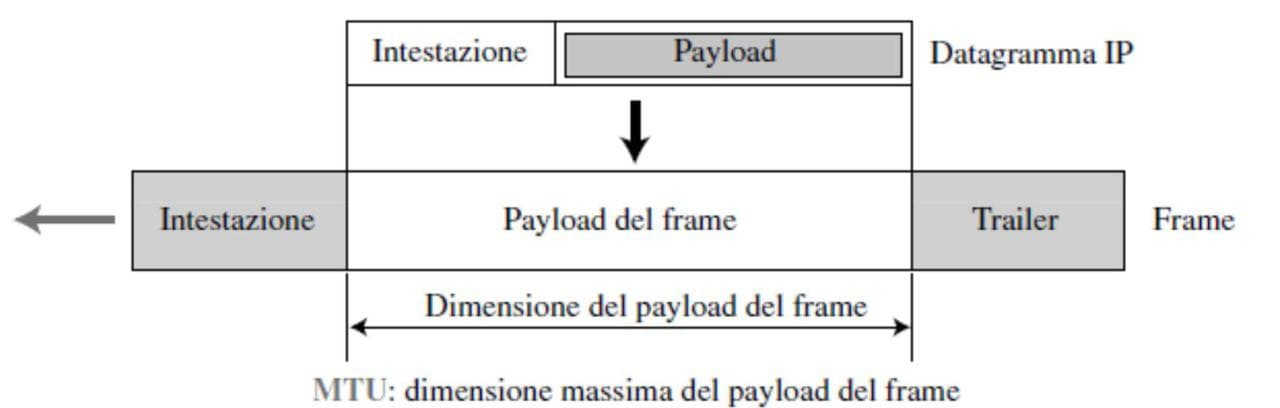
\includegraphics[width = 0.8\textwidth]{immagini/Frammentazione.jpg}
    \caption*{Maximum Transfer Unit (MTU)}
\end{figure}

Quando un datagramma IP viene frammentato ogni frammento ha la propria intestazione, nella maggior parte dei casi i campi dell'intestazione sono uguali rispetto al datagramma originario ma alcuni devono essere cambiati.\
Un datagramma frammentato può essere a sua volta frammentato se incontra una rete con un MTU ancora più piccola.\
In altre parole un datagramma può essere frammentato più volte prima di raggiungere la sua destinazione finale.

Un datagramma può essere frammentato dall'host sorgente o da qualsiasi altro router lungo il percorso verso la destinazione.\
Il \emph{riassemblaggio} del datagramma, tuttavia, viene fatto solo dall'host di destinazione, in quanto ogni frammento diventa un datagramma indipendente.

I diversi frammenti del datagramma originario possono viaggiare lungo percorsi differenti; questi percorsi non sono prevedibili e controllabili a priori ma, alla fine, tutti i frammenti che appartengono allo stesso datagramma dovrebbero arrivare all'host di destinazione finale.\
Oltretutto, il riassemblaggio dei pacchetti durante il percorso provocherebbe una significativa perdita di efficienza.

Quando parliamo di frammentazione non intendiamo solamente che il payload del datagramma IP viene frammentato.\
Infatti, la maggior parte dell'intestazione, ad eccezione di alcune opzioni, deve essere copiata nell'intestazione di tutti i frammenti.\
L'host o il router che frammenta un datagramma IP deve cambiare i valori di tre campi dell'intestazione:\ i flag, lo scostamento di frammentazione e la lunghezza totale.\
Il resto dei campi dell'intestazione deve invece essere solamente copiato.\
Naturalmente il valore del checksum va ricalcolato ad ogni hop indipendentemente dalla frammentazione.

\paragraph{\emph{Campi relativi alla frammentazione}}
Abbiamo detto in precedenza che tre campi nell'intestazione del datagramma IP si riferiscono alla frammentazione:\ \emph{identificazione}, \emph{flag} e \emph{scostamento} di frammentazione (\emph{offset}).

Il \emph{campo identificazione}, da 16 bit, identifica un datagramma che ha origine da un host sorgente.\
La combinazione tra indirizzo IP sorgente e campo identificazione deve definire in modo unico un datagramma quando lascia l'host sorgente.\
Per garantire l'unicità, il protocollo IP utilizza un contatore per etichettare i datagrammi.\
Il contatore viene inizializzato a un numero positivo.\
Quando il protocollo IP invia un datagramma, copia il valore corrente del contatore nel campo identificazione ed incrementa il contatore di uno.\
Quando un datagramma viene frammentato il valore del campo identificazione viene copiato in tutti i frammenti ottenuti.\
In altre parole tutti i frammenti hanno lo stesso numero di identificazione, che è anche lo stesso del datagramma originale.\
Il numero d'identificazione aiuta la destinazione a riassemblare il datagramma.\
Esso sa che tutti i frammenti con lo stesso valore d'identificazione vanno assemblati in un unico datagramma IP.

Il \emph{campo flag}, da 3 bit, in realtà definisce tre flag distinti, ognuno composto da un singolo bit.\
Il bit all'estrema sinistra è riservato (non viene attualmente usato).\
Il secondo bit è definito \emph{do not fragment} (non frammentare).\
Se il suo valore è 1 allora il dispositivo non deve frammentare il datagramma.\
Se non è in grado di trasmettere il datagramma attraverso nessuna delle reti fisiche allora lo scarta ed invia un messaggio d'errore ICMP all'host sorgente.\
Se il suo valore è 0, se necessario, il datagramma può essere frammentato.\
Il terzo bit detto \emph{more fragments}, nel caso sia impostato a 1 indica che questo datagramma non è l'ultimo frammento della serie e che ci sono altri frammenti dopo di lui.\
In altre parole non si tratta dell'ultimo frammento di un datagramma originario.\
Se il suo valore è 0 significa che è l'ultimo (o l'unico) frammento.

Il \emph{campo scostamento di frammentazione (offset)}, da 13 bit, mostra la posizione relativa di questo frammento rispetto all'intero datagramma.\
È l'offset dei dati nel datagramma originario misurato in unità di 8 byte.\
Questo avviene perché la lunghezza del campo offset è di soli 13 bit e non può rappresentare una sequenza di byte maggiore di 8191.\
Ciò costringe gli host o i router che frammentano i datagrammi a scegliere la dimensione dei frammenti in modo che sia divisibile per 8, ad esclusione ovviamente dell'ultimo frammento originato dalla suddivisione di un datagramma.

\subsection{Indirizzi IPv4}

L'identificatore usato dal protocollo IP nella pila TCP/IP per individuare il collegamento di ciascun dispositivo ad Internet è chiamato indirizzo Internet (Internet Address) o indirizzo IP.\
Un indirizzo IPv4 è un indirizzo formato da 32 bit che definisce in modo unico e universale il collegamento di un host o un router ad Internet.\
L'indirizzo IP è l'indirizzo del collegamento, non dell'host o del router, in quanto se il dispositivo viene spostato in un'altra rete, molto probabilmente, l'indirizzo IP verrà cambiato.

Gli indirizzi IP sono unici nel senso che ogni indirizzo definisce uno e un solo collegamento ad Internet.\
Se un dispositivo ha due collegamenti ad Internet, ad esempio tramite due reti diverse, allora avrà due indirizzi IPv4 distinti.\
Gli indirizzi IPv4 sono universali nel senso che ciascun host che vuole collegarsi a Internet deve necessariamente farne uso.

\subsubsection{\emph{Spazio degli indirizzi (address space)}}

Un protocollo come l'IPv4 che utilizza degli indirizzi ha bisogno di definire uno spazio di indirizzi, cioè il numero totale di indirizzi utilizzati dal protocollo.\
Se un protocollo usa \emph{b} bit per rappresentare un indirizzo, lo spazio degli indirizzi è pari a 2\textsuperscript{\emph{b}} perché ogni bit può assumere solo due valori distinti (0 o 1).\
IPv4 usa indirizzi a 32 bit, il che significa che lo spazio degli indirizzi è 2\textsuperscript{32} o 4.294.967.296 (più di quattro miliardi).\
Se non ci fosse alcuna restrizione, oltre 4 miliardi di dispositivi potrebbero essere collegati a Internet.

\subsubsection{\emph{Notazione}}

Esistono tre notazioni comunemente usate per rappresentare gli indirizzi IPv4:\ la notazione binaria (base 2), la notazione decimale puntata (base 256) e quella esadecimale (base 16).\
Nella \emph{notazione binaria} un indirizzo IPv4 viene rappresentato con 32 bit.\
Per facilitare la lettura dell'indirizzo normalmente vengono inseriti uno o più spazi tra ogni ottetto (8 bit).\
Spesso ci si riferisce a ciasun ottetto come ad un byte.\
Per rendere l'indirizzo IPv4 più compatto e facile da leggere normalmente viene scritto in forma decimale, con un punto che separa i byte.\
Questo formato viene definito \emph{notazione decimale puntata} (\emph{dotted-decimal notation}).\
Da notare che siccome ogni byte (ottetto) è formato da soli 8 bit, ogni numero della notazione decimale puntata è compreso tra 0 e 255.\
A volte è possibile trovare un indirizzo IPv4 espresso in notazione esadecimale.\
In questo caso ogni cifra esadecimale equivale a quattro bit.\
Ciò significa che un indirizzo a 32 bit ha 8 cifre esadecimale.\
Tale notazione viene spesso utilizzata nella programmazione di rete.

\begin{figure}[H]
    \centering
    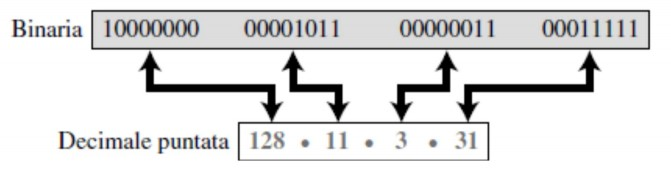
\includegraphics[width = 0.5\textwidth]{immagini/Indirizzi_IPv4.jpg}
    \caption*{Due diverse notazione per l'indirizzamento IPv4}
\end{figure}

\subsubsection{\emph{Gerarchia nell'indirizzamento}}

In ogni rete di comunicazione in cui è prevista la consegna di un messaggio da un mittente ad un destinatario, come una rete telefonica o una rete postale, il meccanismo di indirizzamento è gerarchico.\
In una rete postale, l'indirizzo di spedizione comprende la nazione, la città, la via, il numero civico e il nome del destinatario.\
Allo stesso modo un numero telefonico è diviso in codice nazione, prefisso e numero identificativo.

Anche gli indirizzi IPv4 sono gerarchici, ma divisi in sole due parti.\
La prima parte dell'indirizzo, chiamata \emph{prefisso} (\emph{prefix}), identifica la rete, mentre la seconda parte dell'indirizzo, chiamato \emph{suffiso} (\emph{suffix}), identifica il nodo nella rete (o meglio il collegamento di un dispositivo a Internet).

\begin{figure}[H]
    \centering
    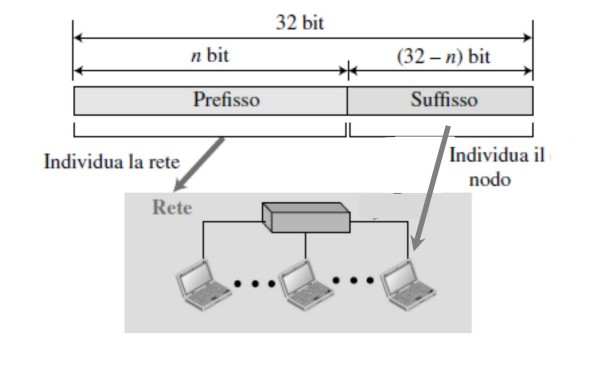
\includegraphics[width=0.6\textwidth]{immagini/prefissi_suffissi.jpg}
    \caption*{Gerarchia nell'indirizzamento}
\end{figure}

Un prefisso può avere una lunghezza fissa o variabile.\
Il sistema di identificazione delle reti in IPv4 è stato inizialmente progettato come prefisso a lunghezza fissa.\
Questo schema, che ormai è obsoleto, viene indicato come indirizzamento con classi (\emph{classful addressing}).\
Il nuovo schema, chiamato indirizzamento senza classi (\emph{classless addressing}), usa un prefisso di rete di lunghezza variabile.

\subsubsection{\emph{Indirizzamento con classi}}

Come detto in precedenza, inizialmente l'indirizzamento IPv4 era stato progettato con un prefisso di lunghezza fissa, ma vista la necessità di supportare sia reti piccole che grandi, al posto di una sola lunghezza di prefisso ne erano state previste 3 ($n =8$, $ n=16 $ e $n=24 $).\
L'intero spazio degli indirizzi era stato diviso in cinque classi (classe A, B, C, D ed E).\
Questo schema è ora definito come \emph{indirizzamento con classi} (\emph{classful addressing}).

\begin{figure}[H]
    \centering
    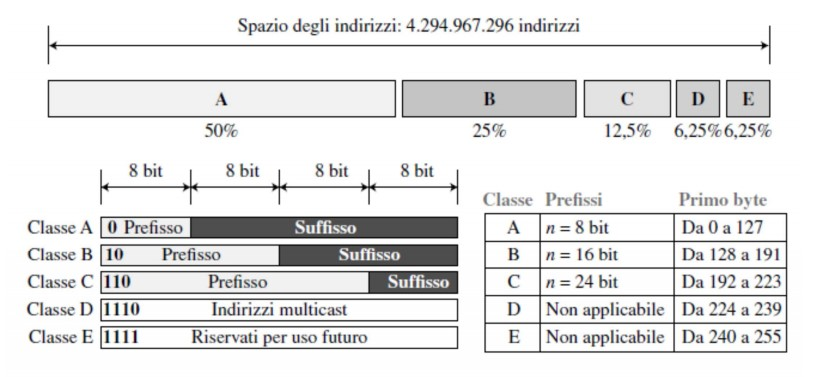
\includegraphics[width = 0.8\textwidth]{immagini/ClassiIP.jpg}
    \caption*{Suddivisione dello spazio degli indirizzi nell'indirizzamento con classi}
\end{figure}

Nella classe A la lunghezza della parte di rete è di 8 bit, ma siccome il primo bit, che è 0, identifica il tipo di classe, possiamo avere solo sette bit per l'identificazione delle reti.\
Ciò significa che ci sono $2^7=128$ reti al mondo che possono avere un indirizzo di classe A.

Nella classe B la lunghezza della parte di rete è di 16 bit, ma siccome i primi due bit, che sono (10)\textsubscript{2} identificano la classe, possiamo avere solo 14 bit per identificare reti.\
Ciò significa che ci sono solo $2^{14} = 16.384$ reti al mondo che possono avere un indirizzo di classe B.

Tutti gli indirizzi che iniziano con (110)\textsubscript{2} appartengono alla classe C, nella quale la lunghezza della parte di rete è di 24 bit, ma siccome tre bit definiscono la classe, possiamo avere solo 21 bit per identificare le reti.\
Ciò significa che ci sono $2^{21}=2.097.152$ reti al mondo che possono avere un indirizzo di classe C.

Gli indirizzi che iniziano con (1110)\textsubscript{2} appartengono alla classe D, una classe che non è divisa in prefisso e suffisso ed è usata per gli indirizzi di tipo multicast.\
Infine, la classe E raccoglie tutti gli indirizzi che iniziano con (1111)\textsubscript{2}.\
Come per la classe D, la classe E non è divisa in prefisso e suffisso ed è riservata per uso futuro.

\paragraph{\emph{Esaurimento degli indirizzi}}

La ragione per cui l'indirizzamento con classi è diventato obsoleto è l'esaurimento degli indirizzi.\
Siccome gli indirizzi non sono stati assegnati in modo appropriato, Internet ha dovuto affrontare il problema dell'esaurimento degli indirizzi disponibili per società ed individui che volevano collegarsi in rete.\
Per comprendere meglio il problema pensiamo alla classe A.\
Tale classe può essere assegnata solo a 128 organizzazioni al mondo, ma a causa della struttura della classe A ognuna deve avere un singola rete con 16.777.216 nodi (computer collocati in questa unica rete).\
Siccome ci sono ben poche organizzazioni così grandi, la maggior parte degli indirizzi in questa classe è andata sprecata (gran parte degli indirizzi erano assegnati ma rimanevano inutilizzati).\
Gli indirizzi di classe B sono stati progettati per le organizzazioni di media dimensione, ma anche in questo caso molti degli indirizzi sono rimasti inutilizzati.\
Gli indirizzi di classe C hanno un difetto di progettazione completamente diverso.\
Il numero di indirizzi disponibili in ogni rete (256) era talmente piccolo che la maggiore parte delle organizzazioni non lo trovavano adeguato per le proprie esigenze.\
Infine, gli indirizzi di classe E erano riservati per uso futuro, sprecando l'intera classe.

\paragraph{\emph{Subnetting e supernetting}}

Per mitigare il problema dell'esaurimento degli indirizzi sono state proposte due strategie che, in certa misura, sono state anche implementate:\ il subnetting e il supernetting.\
Nel subnetting un blocco di classe A o B viene diviso in varie sottoreti (subnet).\
Ogni subnet ha un prefisso di lunghezza maggiore rispetto alla rete originale.\
Per esempio se una rete in classe A viene suddivisa in quattro subnet, ogni subnet ha un prefisso di n\textsubscript{sub} = 10.\
Il vantaggio è che se in una rete non vengono utilizzati tutti gli indirizzi, il subnetting consente di dividere gli indirizzi disponibili tra varie organizzazioni.\
Questa idea non ha funzionato in quanto la maggior parte delle grandi organizzazioni non era disponibile a dividere il proprio blocco di indirizzi per darne alcuni ad organizzazioni più piccole.

Mentre il subnetting è stato ideato per dividere un grande blocco di indirizzi in blocchi più piccoli, il supernetting è stato ideato per combinare numerosi blocchi di classe C in un blocco più grande, che potesse soddisfare organizzazioni per le quali un blocco di classe C (256) era troppo piccolo.\
Questa idea nella pratica non ha funzionato perché complicava il routing dei pacchetti.

\paragraph{\emph{Vantaggi dell'indirizzamento con classi}}

Anche se l'indirizzamento con classi presentava numerosi problemi ed è diventato obsoleto, aveva un vantaggio:\ una volta individutato un indirizzo IP, si poteva facilmente risalire alla classe dell'indirizzo e, siccome la lunghezza del prefisso di ogni classe è fissa, scoprire immediatamente la lunghezza del prefisso.\
In altre parole, la lunghezza del prefisso nell'indirizzamento con classi fa parte dell'indirizzo stesso, non c'è quindi la necessità di aggiungere altre informazioni per determinare la parte di prefisso e quella di suffisso.

\subsubsection{\emph{Indirizzamento senza classi}}

Il subnetting e il supernetting nell'indirizzamento con classi non erano realmente in grado di risolvere il problema dell'esaurimento degli indirizzi.\
Con la crescita di Internet era chiaro che, come soluzione a lungo termine, sarebbe servito uno spazio degli indirizzi più grande.\
Tuttavia, questa soluzione richiede necessariamente che la lunghezza degli indirizzi IP venga aumentata, il che significa anche che il formato dei datagrammi IP deve essere modificato.\
Anche se la soluzione a lungo termine è già stata ideata ed implementata (IPv6), è stata studiata anche una soluzione a breve termine.\
In questa soluzione si continua a usare lo stesso spazio degli indirizzi ma si cambia la loro distribuzione, attraverso un approccio più equo.\
La soluzione a breve termine è ancora basata sugli indirizzi IPv4 ma non fa più uso della divisione in classi.\
In altre parole la suddivisione in classi è stata rimossa per compensare la scarsità di indirizzi disponibili.

C'è stata un'altra motivazione che ha favorito l'indirizzamento senza classi.\
Negli anni '90 sono emersi gli Internet Service Provider (ISP).\
Un ISP è un'organizzazione che fornisce accesso Internet a individui, piccole imprese e aziende di medie dimensioni che non vogliono entrare direttamente a far parte di Internet e fornire a loro volta servizi Internet.\
Sono aziende che per semplicità vogliono solamente utilizzare i servizi messi a disposizione da un ISP.\
Un ISP ottiene quindi un insieme piuttosto ampio di indirizzi e lo suddivide in gruppi di indirizzi (con dimensione 1, 2, 4, 8, 16, etc.), fornendo questi gruppi di indirizzi ai suoi clienti a seconda delle loro tipologie ed esigenze.

Nel 1996 gli enti di gestione di Internet hanno annunciato una nuova struttura chiamata \emph{indirizzamento senza classi}.\
In questa forma di indirizzamento vengono utilizzati dei blocchi di lunghezza variabile che non appartengono a nessuna classe.\
Possiamo avere un blocco da 1, 2, 4, 128 indirizzi e così via.

Nell'indirizzamento senza classi l'intero spazio degli indirizzi è diviso in blocchi di lunghezza variabile.\
Il prefisso in un indirizzo definisce il blocco (individua la rete):\ il suffisso definisce il nodo (individua il dispositivo).\
In teoria possiamo avere un blocco di 2\textsuperscript{0}, 2\textsuperscript{1}, 2\textsuperscript{2}, \dots, 2\textsuperscript{32} indirizzi.\
Una delle restrizioni, di cui parleremo più avanti, è che il numero degli indirizzi in un blocco deve essere una potenza di 2.\
Ad un'organizzazione si può quindi assegnare un blocco di indirizzi di dimensione adeguata alle sue esigenze.

A differenza dell'indirizzamento con classi, la lunghezza del prefisso nell'indirizzamento senza classi è variabile.\
Possiamo avere una lunghezza del prefisso che va da 0 a 32 bit.\
La dimensione della parte di rete è inversamente proporzionale alla lunghezza del prefisso.\
Un prefisso piccolo implica una rete più grande (con molti nodi al suo interno); un prefisso grande implica una rete più piccola (con pochi nodi).

Bisogna sottolineare che l'idea dell'indirizzamento senza classi si può applicare facilmente all'indirizzamento con classi.\
Un indirizzo di classe A si può pensare come un indirizzo senza classi nel quale la lunghezza del prefisso è di 8 bit.\
Un indirizzo di classe B è un indirizzo senza classi con prefisso di 16 bit e così via.\
In altre parole l'indirizzamento con classi è un caso speciale dell'indirizzamento senza classi.

\paragraph{\emph{Lunghezza del prefisso:\ notazione slash (barra)}}
La prima domanda cui dobbiamo rispondere nell'indirizzamento senza classi è come trovare la lunghezza del prefisso di un determinato indirizzo.\
Siccome la lunghezza del prefisso non è più parte integrante dell'indirizzo è necessario aggiungere questa informazione in modo separato.\
In questo caso la lunghezza del prefisso, \emph{n}, viene aggiunta all'indirizzo separata da una barra (slash).\
La numerazione viene informalmente definita notazione slash e formalmente \emph{classless interdomain routing} (\emph{CIDR}).

In altre parole, un indirizzo nell'indirizzamento senza classi non è in grado di definire da solo il blocco (o la rete) a cui appartiene, è necessario indicare esplicitamente anche la lunghezza del prefisso.

\begin{figure}[H]
    \centering
    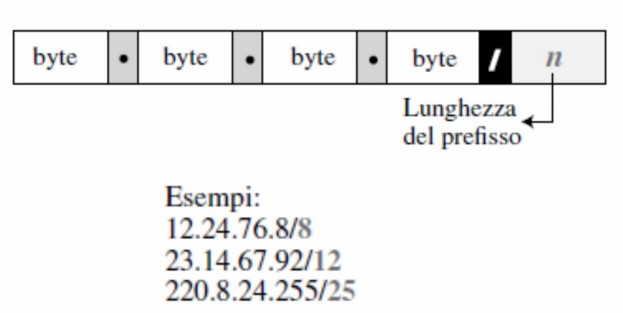
\includegraphics[width = 0.5\textwidth]{immagini/Notazione_slash.jpg}
    \caption*{Numerazione slash (CIDR).}
\end{figure}

\paragraph{\emph{Estrazione delle informazioni da un indirizzo}}
Dato un indirizzo IP appartenente ad un blocco di indirizzi, normalmente vogliamo ricavare tre informazioni riguardo il suo blocco di appartenenza:\ il numero di indirizzi che contiene, il primo indirizzo del blocco e l'ultimo.\
Siccome la lunghezza del prefisso, \emph{n}, è nota, possiamo facilmente ottenere queste tre informazioni.

\begin{enumerate}
    \item Il numero di indirizzi nel blocco è dato da $N = 2^{32-n}$.
    \item Per trovare il primo indirizzo, teniamo invariati i primi \emph{n} bit partendo da sinistra e impostiamo a 0 tutti i bit restanti a destra (sono $32-n$).
    \item Per trovare l'ultimo indirizzo, teniamo invariati i primi \emph{n} bit partendo da sinistra e impostiamo a 1 tutti i bit restanti a destra (anche in questo caso sono $32-n$).
\end{enumerate}

\begin{figure}[H]
    \centering
    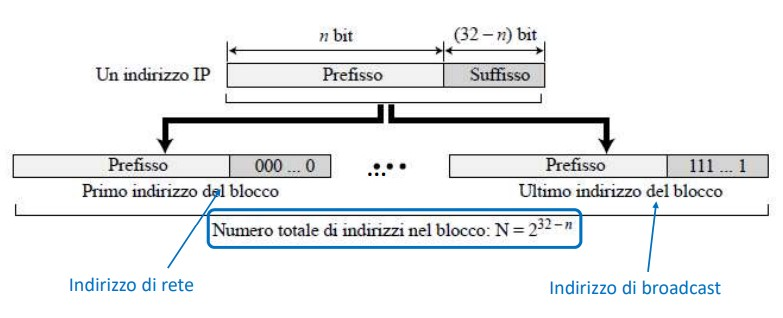
\includegraphics[width = 0.8\textwidth]{immagini/Classless_addressing.jpg}
    \caption*{Estrazione delle informazioni nell'indirizzamento senza classi.}
\end{figure}

\paragraph{\emph{Maschera dell'indirizzo (address mask)}}

Un altro modo per trovare il primo e l'ultimo indirizzo del blocco è usare la maschera dell'indirizzo (address mask), cioè un numero composto da 32 bit in cui i primi \emph{n} bit a sinistra sono impostati a 1 e il resto dei bit ($32-n$) sono impostati a 0.\
Il motivo principale per utilizzare una notazione di questo tipo è che può essere usata da un programma per calcolare in modo efficiente le informazioni di un blocco, usando solamente tre semplici operatori sui bit:\ NOT, AND e OR.

\begin{enumerate}
    \item Il numero degli indirizzi nel blocco è N = \textbf{NOT} (maschera) +1;
    \item Il primo indirizzo nel blocco = (qualsiasi indirizzo del blocco) \textbf{AND} (maschera)
    \item L'ultimo indirizzo nel blocco = (qualsiasi indirizzo del blocco) \textbf{OR} (\textbf{NOT}(maschera)).\
\end{enumerate}

\subsubsection{\emph{Indirizzo di rete (network address)}}

Il primo indirizzo, detto \emph{indirizzo di rete} (\emph{network address}), è particolarmente importante in quanto è usato nell'instradamento dei datagrammi verso la rete di destinazione.\
Per il momento supponiamo che Internet sia composta da \emph{m} reti e da un router con \emph{m} interfacce.\
Quando un datagramma giunge al router da un qualsiasi host sorgente, il router deve sapere a quale rete va inviato il datagramma e quindi da quale interfaccia va inviato.\
Quando il datagramma arriva alla rete di destinazione, raggiungerà l'host di destinazione utilizzando un'altra strategia che vedremo solo in seguito.\
Dopo che il network address è stato trovato, il router consulta la sua tabella d'inoltro per trovare l'interfaccia corrispondente dalla quale inviare il datagramma.\
L'indirizzo di rete in realtà è lo strumento per l'identificazione delle reti:\ ogni rete è identificata per mezzo del suo network address.

\subsubsection{\emph{Assegnazione dei blocchi di indirizzi}}

Il problema successivo nell'indirizzamento senza classi è rappresentato dall'assegnazione dei blocchi.\
La responsabilità dell'assegnazione ricade su un ente globale chiamato Internet Corporation of Assigned Names and Numbers (ICANN).\
L'ICANN non assegna indirizzi a singoli utenti Internet, si occupa invece di assegnare grandi blocchi di indirizzi a ISP (o organizzazioni comparabili per dimensione ad un ISP).\
Per il corretto funzionamento del CIDR devono essere applicate due restrizioni al blocco assegnato.

\begin{enumerate}
    \item Il numero degli indirizzi assegnati, \emph{N}, deve essere una potenza di 2.\
          La ragione è che $N=2^{32-n}$ o $n=32-log_2N$.\
          Se \emph{N} non è una potenza di 2, il valore di \emph{n} non sarà intero.
    \item Quando c'è una richiesta per un blocco di indirizzi di una certa dimensione, il blocco assegnato deve essere uno spazio libero contiguo nello spazio degli indirizzi.\
          Tuttavia c'è una restrizione nella scelta del primo indirizzo nel blocco.\
          Il primo indirizzo deve essere divisibile per il numero degli indirizzi nel blocco.\
          La ragione è che il primo indirizzo deve essere composto dal prefisso seguito da ($32-n$) zeri.\
          Il valore decimale del primo indirizzo quindi è
\end{enumerate}

\begin{center}
    Primo indirizzo = (prefisso in decimale) $\cdot 2^{32-n}$ = (prefisso in decimale) $\cdot N$
\end{center}

\paragraph{\emph{Subnetting}}

Più livelli di gerarchia possono essere creati utilizzando il subnetting.\
Un'organizzazione (o un ISP) a cui viene assegnato un blocco di indirizzi può dividerlo in vari sottoblocchi ed assegnare ognuno di questi ad una sottorete (subnet).\
Da notare che nulla vieta all'organizzazione di creare più livelli.\
Una sottorete può essere divisa a sua volta in varie sotto-reti.\
E così via anche per le sottoreti.

All'interno di una rete, le sottoreti vanno progettate con attenzione, in modo da permettere l'instradamento dei datagrammi.\
Supponiamo che il numero totale degli indirizzi assegnato ad un'organizzazione sia N, la lunghezza del prefisso sia \emph{n}, il numero di indirizzi assegnato ad ogni sotto rete sia N\textsubscript{sub} e la lunghezza del prefisso di ogni sottorete sia \emph{n}\textsubscript{sub}.\
Per un funzionamento corretto delle sottoreti è necessario seguire questi passi:

\begin{enumerate}
    \item il numero degli indirizzi in ogni subnetwork deve essere una potenza di 2;
    \item la lunghezza del prefisso di ogni sottorete va calcolata secondo la formula:
          \begin{center}
              $n_{sub} = 32 - log_2N_{sub}$
          \end{center}
    \item l'indirizzo di partenza di ogni sottorete dovrebbe essere divisibile per il numero di indirizzi presenti in quella sottorete.\
          Ciò si può ottenere assegnando come prima cosa gli indirizzi alle sottoreti più grandi.
\end{enumerate}

Dopo aver progettato le sottoreti, le informazioni relative ad ogni sottorete, come il primo e l'ultimo indirizzo, si possono trovare usando il procedimento descritto in precedenza.

\paragraph{\emph{Aggregazione degli indirizzi}}

Uno dei vantaggi della strategia CIDR è la possibilità di \emph{aggregare gli indirizzi} (address aggregation, address summarization, route summarization).\
Quando alcuni blocchi d'indirizzi vengono combinati per creare un blocco più grande, l'instradamento può essere effettuato sulla base del prefisso del blocco combinato.\
L'ICANN assegna un grande blocco di indirizzi a un ISP, l'ISP suddivide il blocco in sottoblocchi più piccoli e li assegna ai propri clienti.

\paragraph{\emph{Indirizzi speciali}}

Prima di terminare l'argomento degli indirizzi IPv4 dobbiamo parlare di cinque indirizzi speciali che vengono usati per scopi particolari:\ l'indirizzo \emph{this-host}, l'indirizzo \emph{limited-broadcast}, l'indirizzo \emph{loopback}, gli indirizzi \emph{privati} e quelli \emph{multicast}.

\begin{itemize}
    \item \textbf{\emph{Indirizzo this-host}}.\
          L'unico indirizzo del blocco \textbf{0.0.0.0/32} viene chiamato indirizzo \emph{this-host} (\emph{questo host}).\
          Viene usato ogni volta che un host ha la necessità di inviare un datagramma IP ma non conosce il proprio indirizzo da usare come indirizzo sorgente.
    \item \textbf{\emph{Indirizzo limited-broadcast}}.\
          L'unico indirizzo nel blocco\\ \textbf{255.255.255.255/32} viene chiamato indirizzo \emph{limited-broadcast}.\
          Viene usato ogni volta che un router o un host devono inviare un datagramma a tutti i dispositivi che si trovano all'interno della rete.\
          I router della rete, bloccano i datagrammi che hanno questo indirizzo come destinazione, in questo modo la sua diffusione sarà limitata alla rete locale.
    \item \textbf{\emph{Indirizzo di loopback}}.\
          Il blocco \textbf{127.0.0.0/8} viene chiamato indirizzo di \emph{loopback}.\
          Un datagramma con uno degli indirizzi in questo blocco come indirizzo di destinazione non lascia mai l'host di spedizione, rimane al suo interno.\
          Questi indirizzi vengono usati per il test e debug del software in esecuzione sull'host locale.\
          Ad esempio è possibile scrivere un programma client e uno server in cui uno degli indirizzi nel blocco sia usato come indirizzo server.\
          Questo permetterà di testare i programmi client e server usando lo stesso host, prima di installarli su computer diversi.
    \item \textbf{\emph{Indirizzi privati}}.\
          Quattro blocchi sono stati riservati come indirizzi privati:\ \textbf{10.0.0.0/8}, \textbf{172.16.0.0/12}, \textbf{192.168.0.0/16}.\

    \item \textbf{\emph{Indirizzi multicast}}.\
          Il blocco \textbf{224.0.0.0/4} è riservato agli indirizzi multicast.
\end{itemize}

\subsubsection{\emph{Dynamic Host Configuration Protocol (DHCP)}}

Abbiamo visto che una grande organizzazione o un ISP possono ricevere un blocco di indirizzi direttamente dell'ICANN e che una piccola organizzazione può riceverlo direttamente da un ISP.\
Dopo che un blocco di indirizzi è stato assegnato ad un'organizzazione, l'amministratore di rete può assegnare manualmente gli indirizzi ai singoli host o router.\
Tuttavia l'assegnazione degli indirizzi può anche essere automatizzata usando il Dynamic Host Configuration Protocol (DHCP).\
Il DHCP è un programma di livello di applicazione, basato sul paradigma client/server, che in pratica aiuta il TCP/IP a livello di rete.

Il DHCP ha una diffusione amplissima in rete e spesso viene definito \emph{protocollo plug-and-play}.\
Può essere usato in molte situazioni.\
Ad esempio, un amministratore di rete può configurare il DHCP per assegnare indirizzi IP permanenti agli host e ai router.\
Il DHCP può anche essere configurato per fornire indirizzi IP temporanei (a richiesta) agli host.\
Quest'ultima modalità è particolarmente utile, ad esempio, per fornire un indirizzo IP temporaneo all'ospite di un hotel che vuole collegare ad Internet il suo laptop o smartphone.\
Inoltre, consente anche ad un ISP cui sono stati assegnati 1000 indirizzi di fornire servizi a 4000 famiglie, supponendo che non più di un quarto dei suoi clienti usi Internet contemporaneamete.

In aggiunta al suo indirizzo IP, un computer necessita anche di conoscere il proprio prefisso di rete (o la maschera di rete dell'indirizzo).\
La maggior parte dei computer ha bisogno anche di altre due informazioni:\ l'indirizzo di un router di default che deve essere usato per comunicare con le altre reti (oltre a quella locale) e l'indirizzo di almeno un server per la risoluzione dei nomi (DNS).\
Riassumendo, normalmente servono quattro informazioni fondamentali:\ l'indirizzo del computer, il prefisso, l'indirizzo del default router e l'indirizzo IP del server dei nomi di dominio.\
DHCP può essere usato per fornire tutte queste informazioni all'host.

\paragraph{\emph{Funzionamento del DHCP}}

\begin{enumerate}
    \item L'host che vuole entrare in rete crea un messaggio di tipo \textbf{DHCPDISCOVER} nel quale solo il campo transaction-ID viene impostato usando un numero generato casualmente.\
          L'host non può impostare alcun altro campo in quanto non ha le informazioni necessarie per farlo.\
          Questo messaggio viene incapsulato in un datagramma utente UDP con porta sorgente impostata a 68 e la porta destinazione impostata a 67, entrambe sono porte note.\
          Il datagramma utente viene quindi incapsulato in un datagramma IP con indirizzo sorgente 0.0.0.0 (``this-host'') e l'indirizzo di destinazione impostato a 255.255.255.255 (indirizzo broadcast).\
          Il motivo è semplice, l'host al momento non conosce né il proprio indirizzo né quello del server.
    \item Il server o i server DHCP (ce ne possono essere più di uno) rispondono con un messaggio di tipo \textbf{DHCPOFFER} nel quale il campo your-IP-address contiene l'indirizzo IP offerto per l'host che ne ha fatto richiesta e il server-IP-address comprende l'indirizzo IP del server.\
          Il messaggio contiene anche un lease time (tempo di concessione), cioè per quanto tempo l'host potrà far uso di quell'indirizzo IP.\
          Questo messaggio di risposta viene incapsulato in un datagramma utente con gli stessi numeri di porta della richiesta, ma ovviamente in ordine inverso.\
          Il datagramma utente a sua volta viene incapsulato in un datagramma IP con l'indirizzo del server come indirizzo IP sorgente, ma l'indirizzo destinazione è ancora un indirizzo broadcast.\
          Questo è utile anche per consentire agli altri server DHCP di ricevere l'offerta e fornire un'offerta migliore, qualora possano.
    \item L'host richiedente riceve una o più offerte e seleziona la migliore.\
          A questo punto l'host deve inviare un messaggio di tipo \textbf{DHCPREQUEST} al server che ha inviato l'offerta migliore.\
          Tutti i campi con valore noto vengono impostati.\
          Il messaggio viene incapsulato in un datagramma utente con numeri di porta uguali al primo messaggio di richiesta.\
          Il datagramma utente viene incapsulato in un datagramma IP con inidirizzi sorgente e destinazione uguali al primo messaggio di richiesta.\
          Questo è necessario per annunciare a tutti gli altri server la cui offerta non è stata accettata.
    \item Infine, il server selezionato risponde con un messaggio di tipo \textbf{DHCPACK} al client se l'indirizzo IP offerto è valido.\
          Se il server non è più in grado di mantenere la sua offerta (per esempio se nel frattempo l'indirizzo è stato offerto ad un altro host), il server invia un messaggio di tipo \textbf{DHCPNACK} e il client deve ripetere il procedimento.\
          Anche questo messaggio è broadcast per far sapere agli altri server se la richiesta è stata accettata o rifiutata.
\end{enumerate}

\begin{figure}[H]
    \centering
    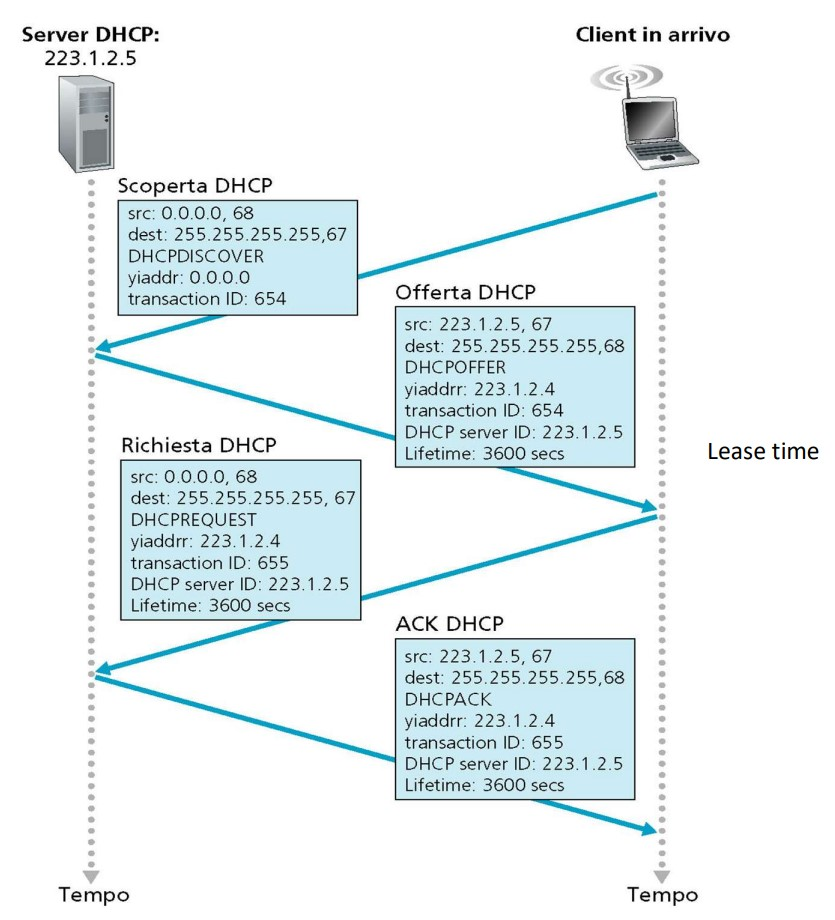
\includegraphics[width=0.7\textwidth]{immagini/DHCP.jpg}
\end{figure}

\subsubsection{NAT}

NAT ovvero Network Address Translation (RFC 2663, 3022), permette di trasmettere su Internet il traffico proveniente da sistemi attestati su sottoreti private, in cui sono assegnati indirizzi IP privati.

L'accesso di una rete privata su Internet è realizzato attraverso un router abilitato alla NAT, questo router \textbf{ha almeno un} indirizzo IP pubblico
\begin{itemize}
    \item Tutto il traffico (datagram) in uscita dal router di accesso ha un indirizzo IP sorgente pubblico, quello del router.
    \item Tutto il traffico in ingresso alla subnet ha come indirizzo IP di destinazione l’indirizzo pubblico del router di accesso.
\end{itemize}
Il router di accesso ha in memoria una tabella di traduzione NAT, le cui righe contengono le associazioni
\begin{center}
    (IP privato, porta) (IP pubblico e porta assegnata dal router)
\end{center}

\begin{figure}[H]
    \centering
    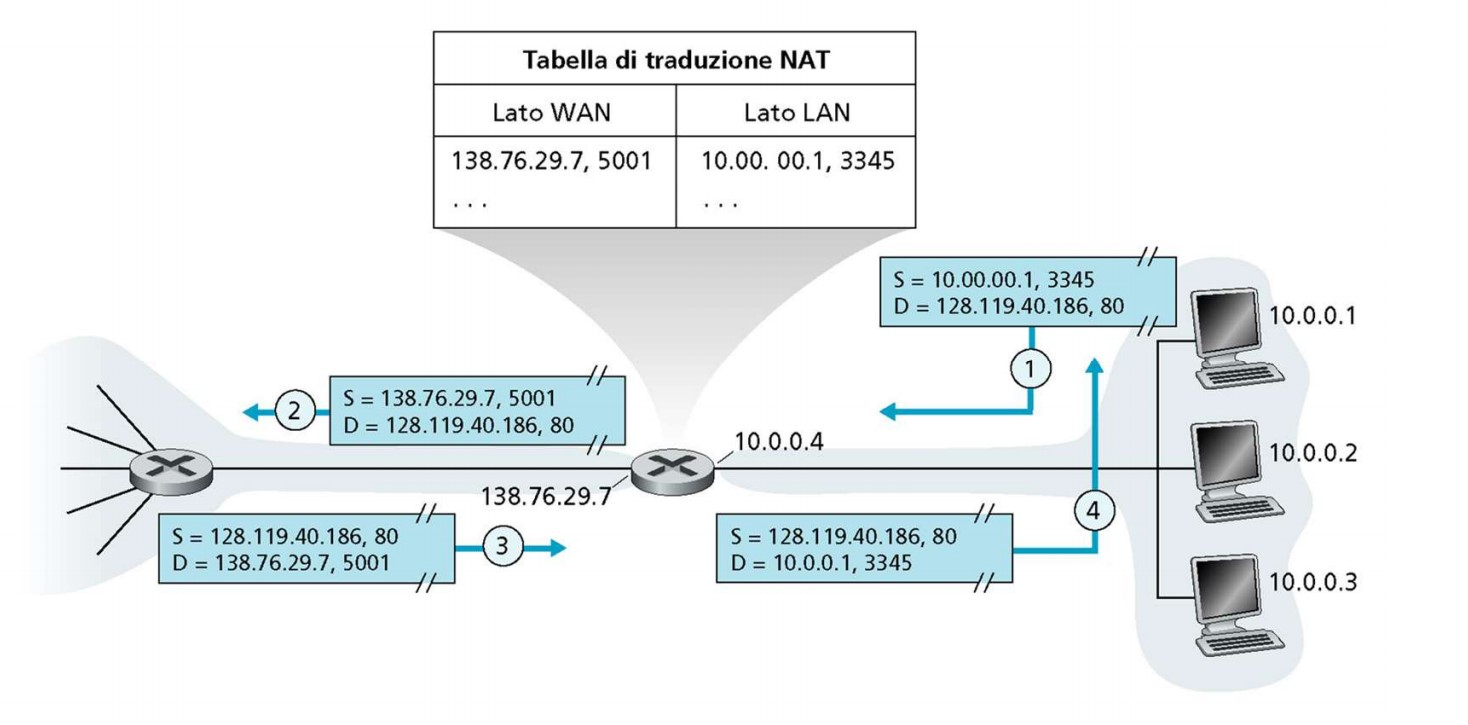
\includegraphics[width=\textwidth]{immagini/NAT.jpg}
    \caption*{Network Address Translation (NAT)}

\end{figure}
\begin{figure}[H]
    \centering
    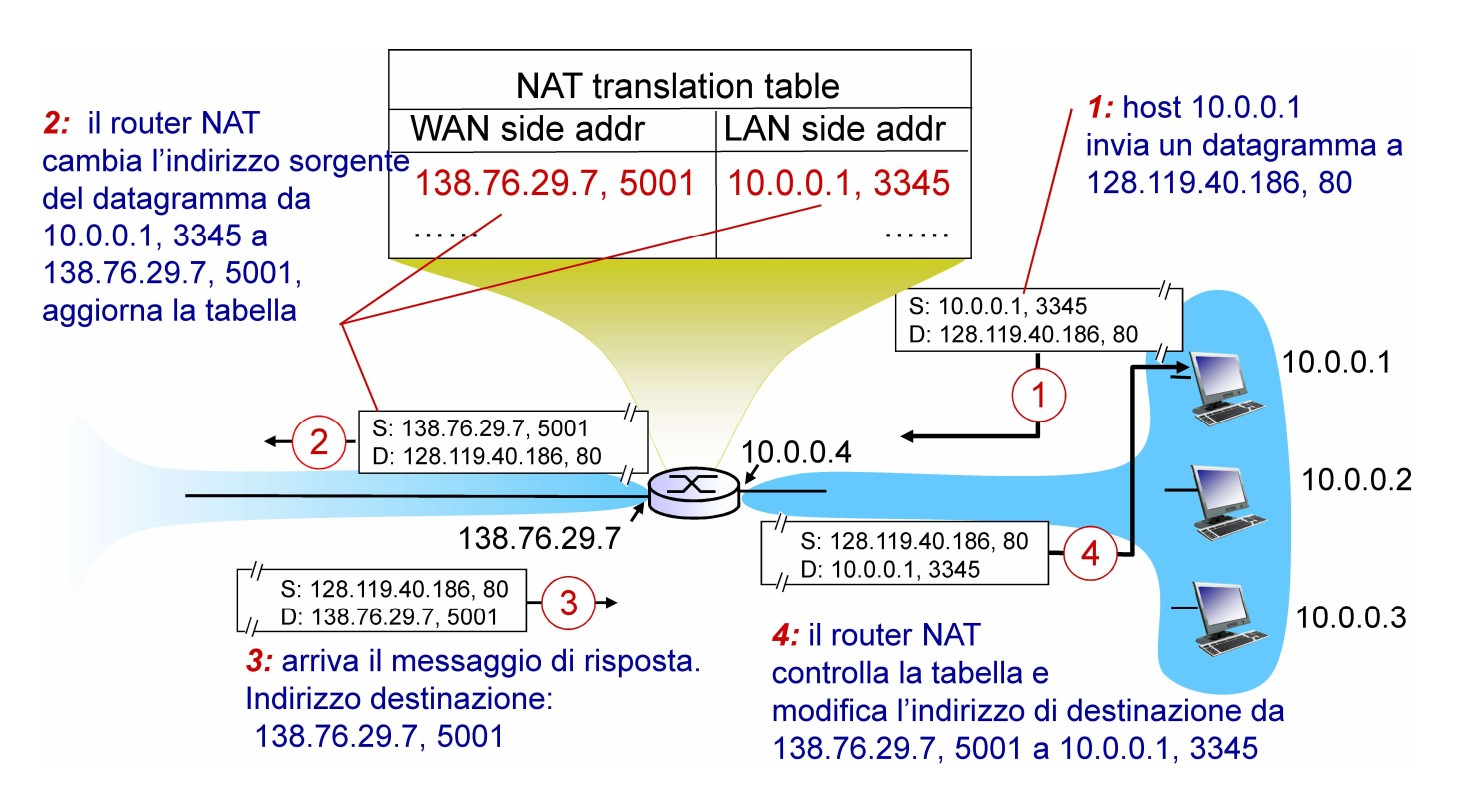
\includegraphics[width=\textwidth]{immagini/NAT2.jpg}
    \caption*{Traduzione dell'indirizzo}
\end{figure}

\subsection{Inoltro dei datagrammi IP}

All'inizio del capitolo è stato discusso il tema dell'inoltro (forwarding) a livello di rete.\
In questa sezione, il concetto sarà esteso per includere anche il ruolo degli indirizzi IP nel forwarding.\
Come detto in precedenza, inoltrare significa collocare il pacchetto nel giusto percorso che lo porterà a destinazione.\
Dato che oggi Internet è costituita da una combinazione di collegamenti (reti), inoltrare significa inviare il pacchetto al salto (hop) successivo (che può essere la destinazione finale o un dispositivo d'interconnessione intermedio).

\subsubsection{\emph{Inoltro basato sull'indirizzo di destinazione}}

Questo approccio richiede che l'host o il router che deve effettuare il forwarding abbia una tabella d'inoltro.\
Quando un host ha un datagramma da inviare o quando un router ha ricevuto un datagramma da inoltrare, esso fa riferimento a questa tabella per trovare il salto successivo in cui inviare il datagramma.

Nell'indirizzamento senza classi, l'intero spazio degli indirizzi è un'unica entità; come dice il nome non ci sono classi.\
Nella pratica ciò significa che l'inoltro richiede una riga di informazioni per ciascun blocco coinvolto.\
Le informazioni nella tabella devono essere cercate in base all'indirizzo di rete (il primo indirizzo nel blocco).\
Sfortunatamente, l'indirizzo di destinazione presente nel datagramma non fornisce alcun indizio in merito all'indirizzo di rete.\
Per risolvere il problema, occorre includere la maschera (\emph{ln}) nella tabella.\
In altre parole, una tabella d'inoltro per l'indirizzamento senza classi deve includere quattro informazioni:\ la maschera, l'indirizzo di rete, il numero dell'interfaccia e l'indirizzo IP del router successivo (quest'ultimo è necessario per trovare l'indirizzo a livello di collegamento del salto successivo).\
Tuttavia, abbiamo visto che spesso le prime due informazioni sono combinate.

Il compito del modulo di forwarding è quello di effettuare le ricerche nella tabella.\
In ciascun riga, gli \emph{n} bit a sinistra dell'indirizzo di destinazione (prefisso) sono lasciati invariati e il resto dei bit (suffisso) sono impostati a 0.\
Se l'indirizzo risultante (chiamato \emph{indirizzo di rete}) combacia con l'indirizzo nella prima colonna, allora l'informazione nelle successive due colonne viene estratta.\
In caso contrario la ricerca continua.\
Normalmente l'ultima riga ha un valore di default nella prima colonna (non mostrato nella figura) che rappresenta tutti gli indirizzi di destinazione che non combaciano le righe precedenti (in generale si dice quindi che è una ``riga di default'').
\begin{figure}[H]
    \centering
    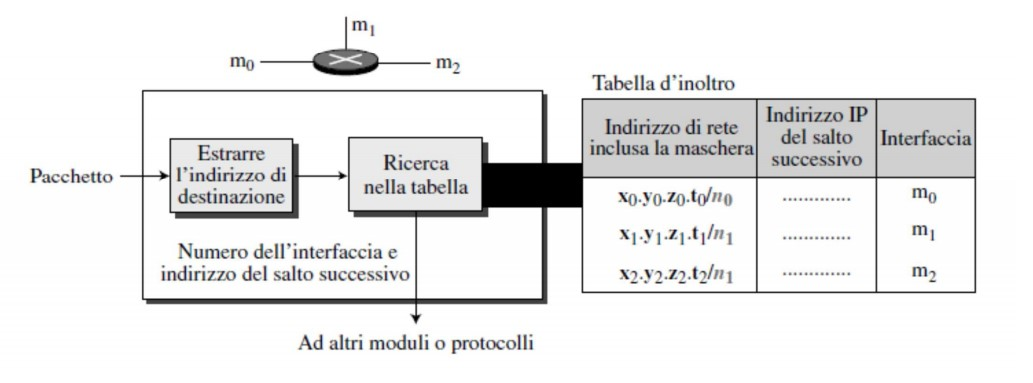
\includegraphics[width=\textwidth]{immagini/Modulo_inoltro.jpg}
    \caption*{Modulo d'inoltro semplificato per l'indirizzamento senza classi}
\end{figure}

\paragraph{Forwarding diretto/indiretto}

L'inoltro può essere di due tipi:\ diretto e indiretto.

Si parla di inoltro diretto quando il pacchetto IP ha come destinazione un host nella propria rete (o subnet) IP.
\begin{itemize}
    \item l'invio è diretto sul destinatario;
    \item l'indirizzo di destinazione a livello link è quello del destinatario (MAC address);
    \item non viene interpellata nessun'altra entità.
\end{itemize}
Nell'inoltro indiretto il pacchetto IP ha come destinazione un host di un'altra rete (o subnet) IP.

\begin{itemize}
    \item Viene delegato l'invio ad ``un altro'';
    \item ``l'altro'' si chiama router;
    \item l'indirizzo di destinazione a livello link è quello del router.
\end{itemize}
Si osserva come, in entrambi i casi, \textbf{condizioni necessarie} perché tutto funzioni sono che:

\begin{itemize}
    \item esista un cammino (funzionante e) diretto, a livello data-link, tra tutti gli host che appartengono ad una stessa sottorete;
    \item ogni host coinvolto abbia un indirizzo IP ``giusto'', cioè con uguale net ID (cioè appartenga alla stessa sottorete) e con host ID univoco nella sottorete.
\end{itemize}
\emph{Le due condizioni insieme diventano condizione necessaria e sufficiente per\-ché la comunicazione ``funzioni''}.

\begin{figure}[H]
    \centering
    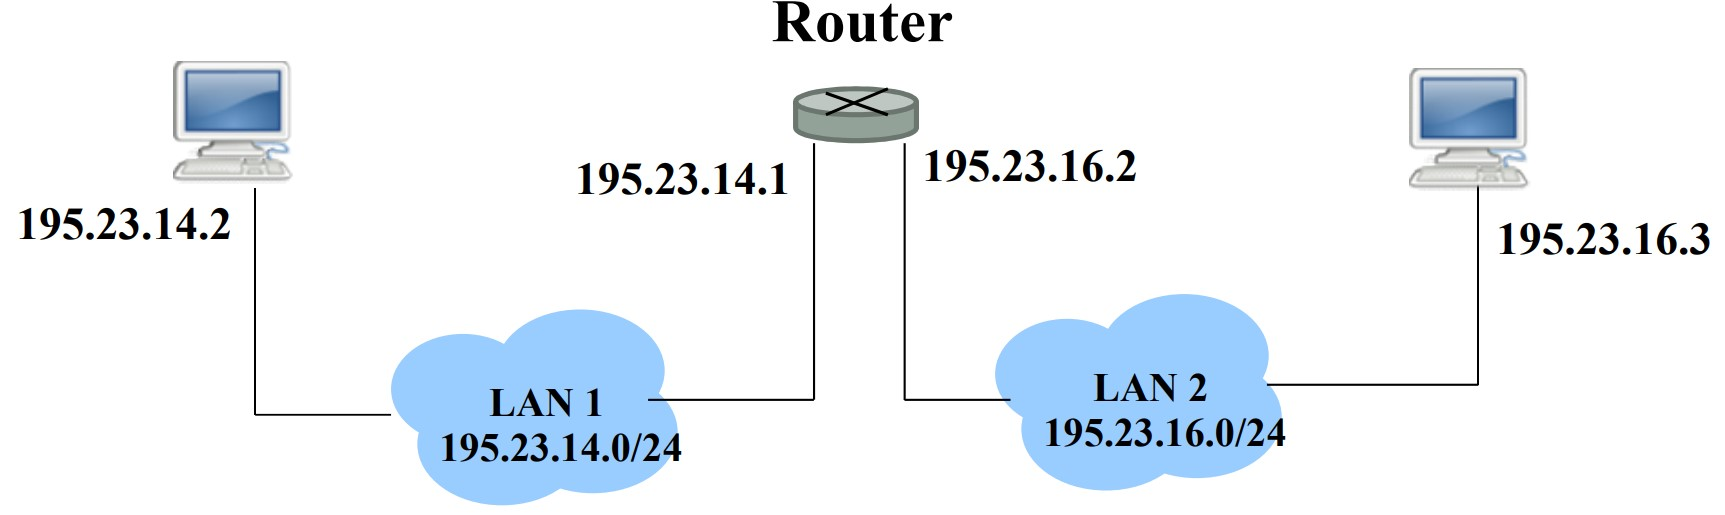
\includegraphics[width=0.8\textwidth]{immagini/Rete_IP.jpg}
    \caption*{Ad ogni interfaccia verso la rete IP viene assegnato un indirizzo IP distinto.\\ Il router è un apparato che svolge funzioni di instradamento a livello IP.\
        Esso legge gli indirizzi IP, consulta la propria tabella di forwarding e decide dove mandare il pacchetto IP.}
\end{figure}

\begin{figure}[H]
    \centering
    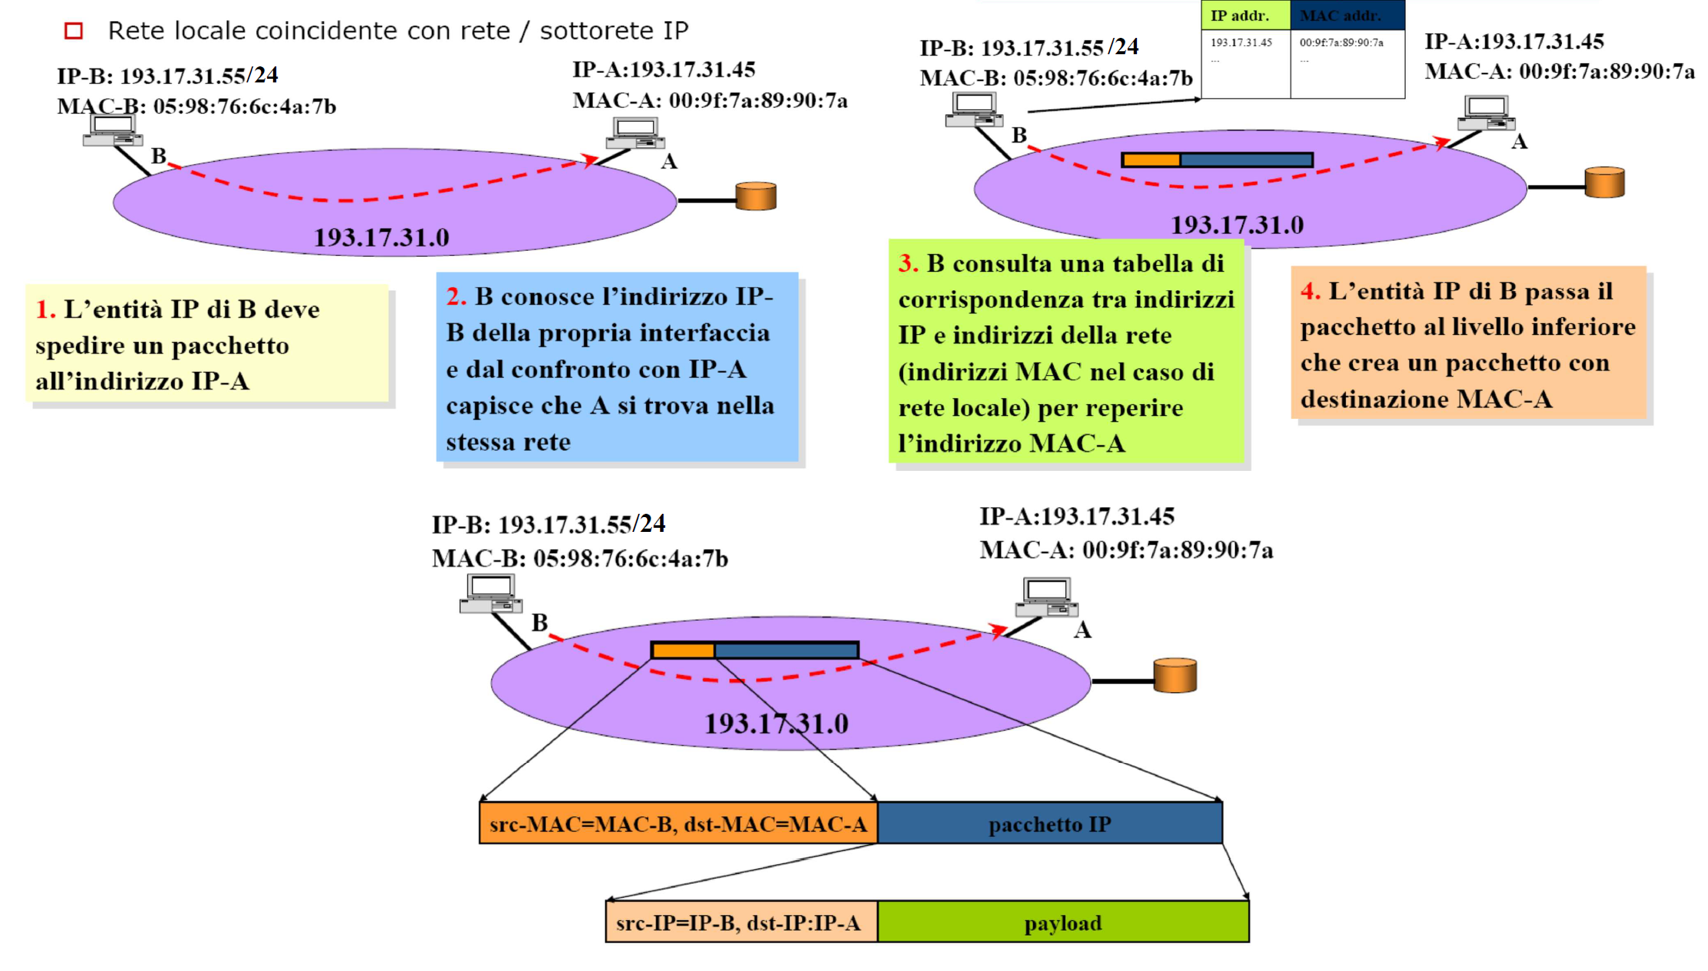
\includegraphics[width=\textwidth]{immagini/Inoltro_diretto.png}
    \caption*{Inoltro diretto}
\end{figure}

\begin{figure}[H]
    \centering
    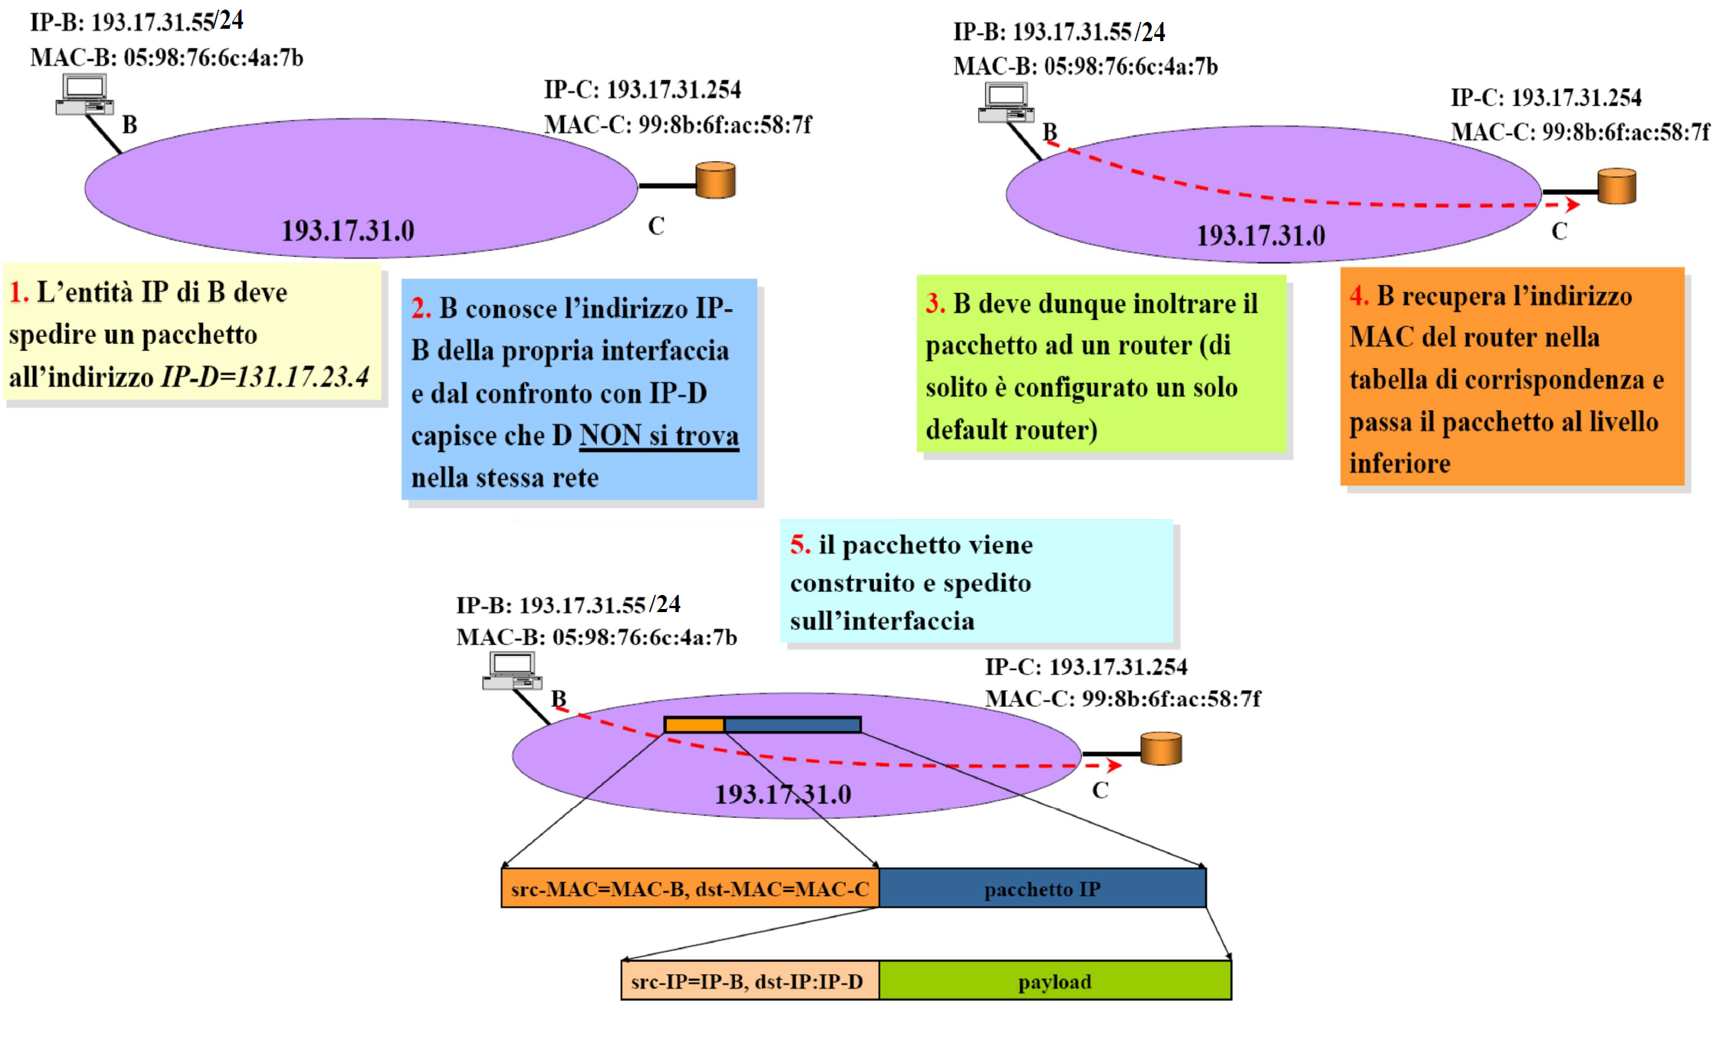
\includegraphics[width=\textwidth]{immagini/Inoltro_indiretto.png}
    \caption*{Inoltro indiretto}
\end{figure}

\paragraph{\emph{Aggregazione degli indirizzi}}

Quando viene utilizzato l'indirizzamento con classi, nella tabella d'inoltro è presente solamente una riga per ciascuna rete esterna all'organizzazione a cui appartiene il router.\
La riga è in grado di rappresentare pienamente la rete esterna anche se questa fa uso di subnetting.\
Quando un datagramma arriva al router, questo verifica la riga corrispondente ed effettua l'inoltro in base alle informazioni ricavate.\
Quando invece si utilizza l'indirizzamento senza classi, si assiste ad un aumento del numero delle righe nella tabella d'inoltro.\
Questo perché lo scopo dell'indirizzamento senza classi è proprio quello di dividere lo spazio degli indirizzi in blocchi più piccoli e gestibili.\
L'aumento nel numero delle righe da controllare porta ad un maggior tempo necessario per le ricerche nella tabella d'inoltro.\
Per attenuare questo problema è stato ideato il meccanismo di aggregazione degli indirizzi.

\begin{figure}[H]
    \centering
    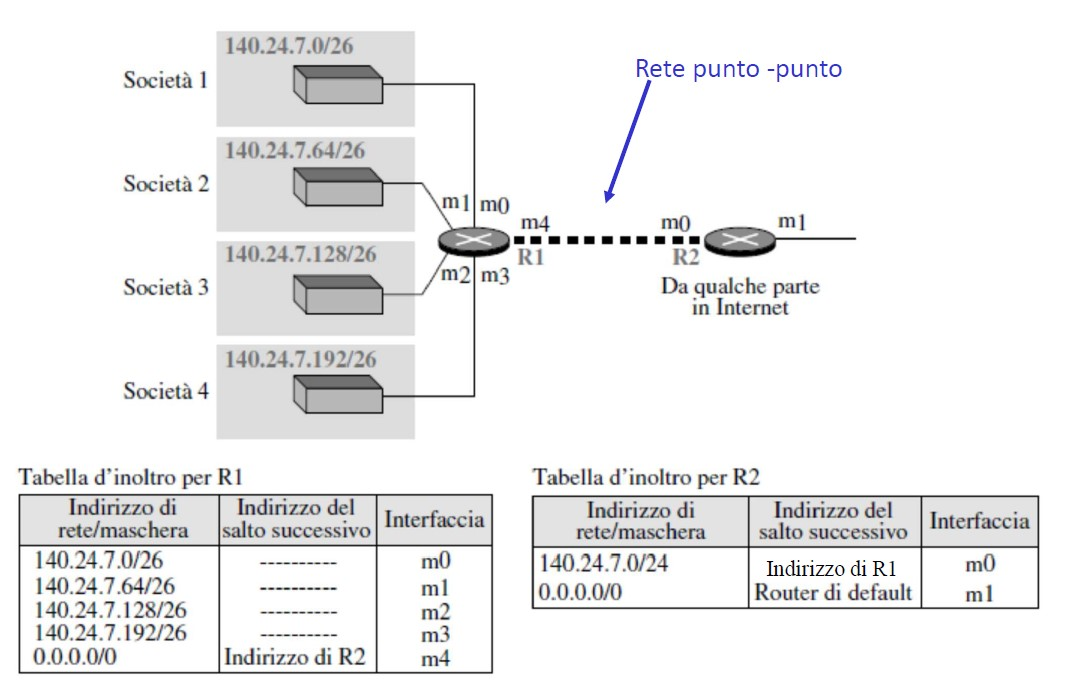
\includegraphics[width=0.9\textwidth]{immagini/Aggrregazione_indirizzi.jpg}
    \caption*{Aggregazione degli indirizzi}
\end{figure}

R1 è connesso alle reti di quattro organizzazioni, ciascuna con un blocco di 64 indirizzi.\
R2 è da qualche parte in Internet, lontano da R1.\
È evidente che R1 ha una tabella d'inoltro più lunga di R2 poiché ciascun datagramma che gli arriva deve essere indirizzato correttamente all'organizzazione appropriata.\
R2, invece, può avere una tabella d'inoltro molto piccola.\
Per R2, qualunque datagramma con indirizzo di destinazione compreso tra 140.24.7.0 e 140.24.7.255 è inviato attraverso l'interfaccia \emph{m\textsubscript{0}}, senza considerare in alcun modo il destinatario specifico (a quale organizzazione dovrà alla fine essere consegnato il datagramma).\
Questo meccanismo è chiamato aggregazione degli indirizzi, poiché i blocchi degli indirizzi di quattro società sono stati aggregati in un solo blocco più grande.\
Nel caso ciascuna organizzazione avesse blocchi di indirizzi che non possono essere aggregati in un blocco più grande (ad esempio blocchi non contigui), R2 sarebbe costretto ad avere una tabella d'inoltro molto più lunga.

\paragraph{\emph{Corrispondenza con la maschera più lunga}}

Che cosa accade se una delle organizzazione nella figura precedente non è geograficamente vicina alle altre tre? Ad esempio, se l'organizzazione 4 non può essere connessa al router R1 per qualche ragione, possiamo ancora utilizzare l'idea di aggregazione di indirizzo e assegnare il blocco 140.24.7.192\slash26 alla società 4? La risposta è sì poiché l'instradamento nell'indirizzamento senza classi sfrutta un altro principio, la \emph{corrispondenza con la maschera più lunga} (\emph{longest mask matching}).\
Questo principio afferma che la tabella d'inoltro viene ordinata dalla maschera più lunga alla maschera più corta.\
In altre parole, se ci sono 3 maschere, \slash27, \slash26 e \slash24, la maschera \slash27 deve essere nella prima riga e la \slash24 deve essere nell'ultima (senza considerare la regola di default).\
Vediamo se questo principio permette di risolvere la situazione nella quale l'organizzazione 4 è separata dalle altre tre.

\begin{figure}[H]
    \centering
    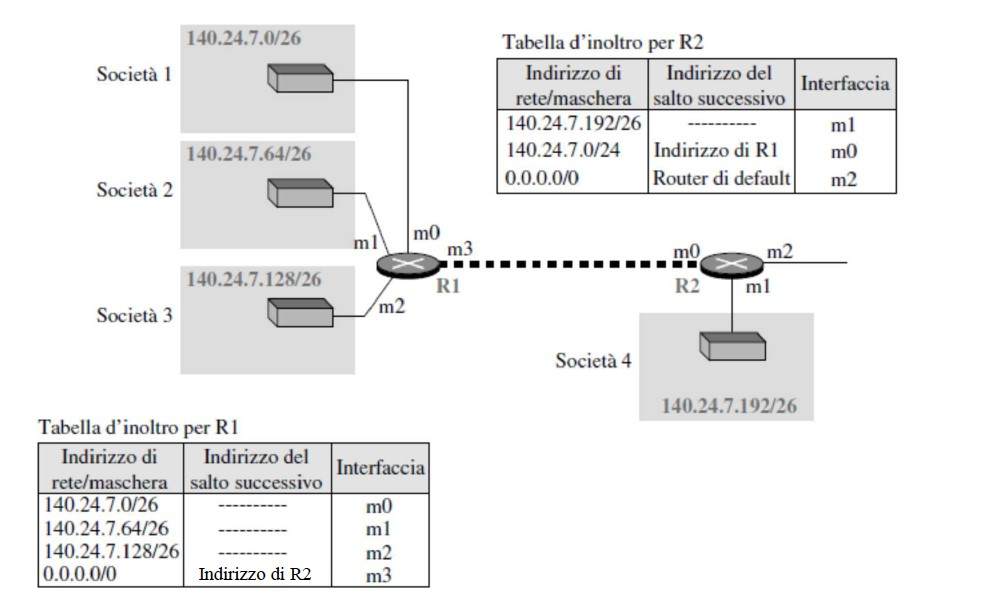
\includegraphics[width=0.9\textwidth]{immagini/Longer_mask.jpg}
    \caption*{Corrispondenza con la maschera più lunga}
\end{figure}

Supponiamo che un pacchetto arrivi al router R2 con indirizzo di destinazione 140.24.7.200.\
La prima maschera nel router R2 è applicata e dà l'indirizzo di rete 140.24.7.192.\
Il datagramma è quindi instradato correttamente all'interfaccia \emph{m\textsubscript{1}} e raggiunge l'organizzazione 4.\
Tuttavia, se la tabella d'inoltro non fosse memorizzata con il prefisso più lungo per primo, applicando la maschera \slash24 si avrebbe un instradamento sbagliato e l'invio del datagramma al router R1.

\paragraph{\emph{Routing gerarchico}}

Per risolvere il problema delle tabelle d'inoltro di dimensione eccessiva è possibile implementare una sorta di gerarchia nelle tabelle d'inoltro.\
Oggi Internet ha una struttura in qualche modo gerarchica, essendo divisa in dorsali e ISP nazionali.\
Gli ISP nazionali sono suddivisi in ISP regionali, che a loro volta sono partizionati in ISP locali.\
Se la tabella d'inoltro ha una qualche forma di gerarchia, analoga all'architettura di Internet, può diminuire di dimensione.

Prendiamo il caso di un ISP locale.\
A un ISP locale può essere assegnato un singolo, ma ampio, blocco di indirizzi con un certa lunghezza di prefisso.\
L'ISP locale può suddividere questo blocco in blocchi più piccoli, di diverse dimensioni, e assegnarli ad utenti individuali e organizzazioni di varia dimensione.\
Se il blocco assegnato all'ISP locale inizia con a.b.c.d/n, l'ISP può creare blocchi che iniziano con e.f.g.h/m dove m può variare per ciascun cliente ed è maggiore di n.

Come può questo ridurre la dimensione della tabella d'inoltro? Molto semplicemente, il resto di Internet non è consapevole di questa divisione (e non c'è bisogno che lo sia).\
Tutti i clienti dell'ISP locale sono individuati come a.b.c.d/n per il resto di Internet.\
Ogni datagramma destinato a uno degli indirizzi in questo blocco piuttosto ampio è instradato all'ISP locale.\
In ogni router del mondo vi è una sola riga per tutti questi clienti; tutti loro appartengono allo stesso gruppo.\
Ovviamente, all'interno dell'ISP locale, il router deve riconoscere i sottoblocchi ed instradare i datagrammi al destinatario giusto.\
Se uno dei clienti non è una grande organizzazione, al suo interno può creare un ulteriore livello gerarchico usando il subnetting e dividendo il suo sottoblocco in blocchi ancora più piccoli.

\begin{figure}[H]
    \centering
    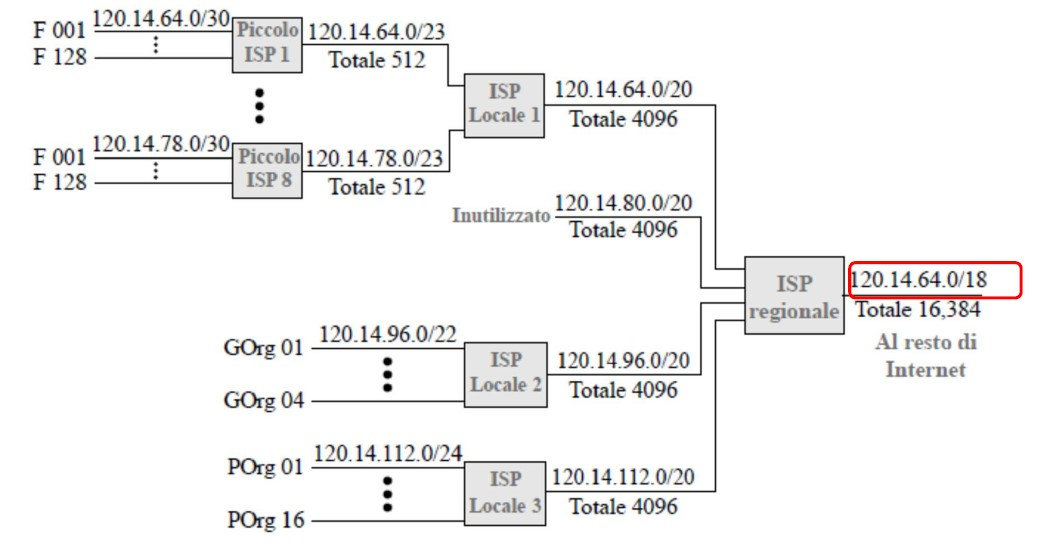
\includegraphics[width=\textwidth]{immagini/Routing_gerarchico.jpg}
    \caption*{Routing gerarchico ed ISP}
\end{figure}

\subsection{ICMPv4}

L'IPv4 non implementa alcun meccanismo per segnalare gli errori o correggerli.\
Cosa accade se qualcosa va storto? Che cosa accade se un router deve scartare un datagramma perché non riesce a trovare un percorso per la destinazione finale o perché il campo time-to-live ha raggiunto il valore zero? Che cosa accade se un host di destinazione non ha ricevuto tutti i frammenti di un datagramma entro un determinato limite di tempo prestabilito? Queste sono tutte situazioni nelle quali si è verificato un errore, ma il protocollo IP non ha meccanismi integrati per renderlo noto all'host mittente.

Inoltre, il protocollo IP è sprovvisto di un meccanismo per effettuare richieste sullo stato di un sistema remoto.\
Ad esempio, un host, può a volte aver bisogno di determinare se un router o un altro host è attivo.\
Altre volte un amministratore di rete può aver bisogno di informazioni relative ad un host o un router.

L'\emph{Internet Control Message Protocol} versione 4 (ICMPv4) è stato creato per porre rimedio a queste carenze.\
ICMP deve essere pensato come la controparte di IP ed è esso stesso un protocollo del livello di rete.\
Tuttavia, i suoi messaggi non vengono passati direttamente al livello di collegamento, come ci si potrebbe aspettare.\
I messaggi ICMP vengono incapsulati all'interno di datagrammi IP prima di essere passati al livello inferiore.\
Quando un datagramma incapsula un messaggio ICMP, il valore del campo protocollo nel datagramma IP è impostato a 1, per indicare che nel payload del datagramma è presente un messaggio ICMP.

\subsubsection{\emph{Messaggi}}

I messaggi ICMPv4 sono suddivisi in due ampie categorie:\ \emph{messaggi di segnalazione errori} e \emph{messaggi di richiesta} (\emph{query messages}).\
I messaggi di segnalazione riportano i problemi che un router o un host (la destinazione) possono incontrare quando elaborano un datagramma IP.\
I messaggi di richiesta, invece, permettono ad un host o ad un amministratore di rete di chiedere informazioni ad un router o ad un host.\
Ad esempio, un host può individuare gli altri host nella rete locale e un router può indicare ad un nodo come reindirizzare i propri datagrammi.

\paragraph{\emph{Formato dei messaggi}}

Un messaggio ICMPv4 ha un'intestazione di 8 byte e una sezione dati di lunghezza variabile.\
Anche se il formato dell'intestazione è diverso per ogni tipo di messaggio, i primi 4 byte sono comuni a tutti.\
Il primo campo, il tipo ICMP, definisce il tipo di messaggio.\
Il campo codice specifica la ragione del particolare tipo di messaggio.\
L'ultimo campo comune è quello del checksum.\
Il resto dell'intestazione è specifico per ciascun tipo di messaggio.\
La sezione dati nei messaggi di errore trasporta informazioni utili per individuare il datagramma originale che ha provocato l'errore.\
Nei messaggi di richiesta invece la sezione dati trasporta informazioni aggiuntive che dipendono dal tipo di interrogazione.

\begin{figure}[H]
    \centering
    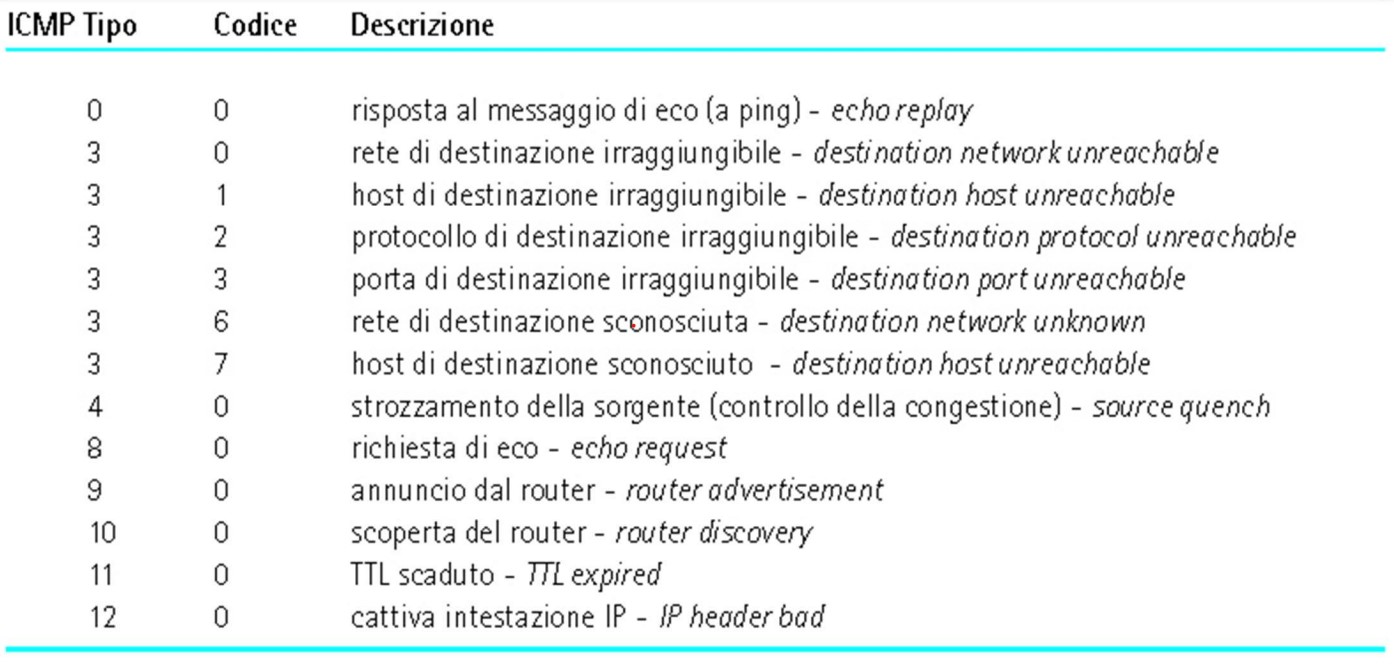
\includegraphics[width=\textwidth]{immagini/Tipi_ICMP.jpg}
    \caption*{Tipi di messaggio ICMP}
\end{figure}

\paragraph{Ping}

Una delle applicazioni che un host può utilizzare per verificare il funzionamento di un altro host è il programma \emph{ping}.\
Il programma \emph{ping} si basa sui messaggi di richiesta e risposta eco dell'ICMP.\
Un host invia una richiesta eco (tipo 8, codice 0) a un altro host che, se attivo, può rispondere con una risposta eco (tipo 0, codice 0).\
In maniera molto grossolana, il programma \emph{ping} può anche misurare l'affidabilità e la congestione del router tra due host inviando una sequenza di messaggi richiesta-risposta.

\begin{figure}[H]
    \centering
    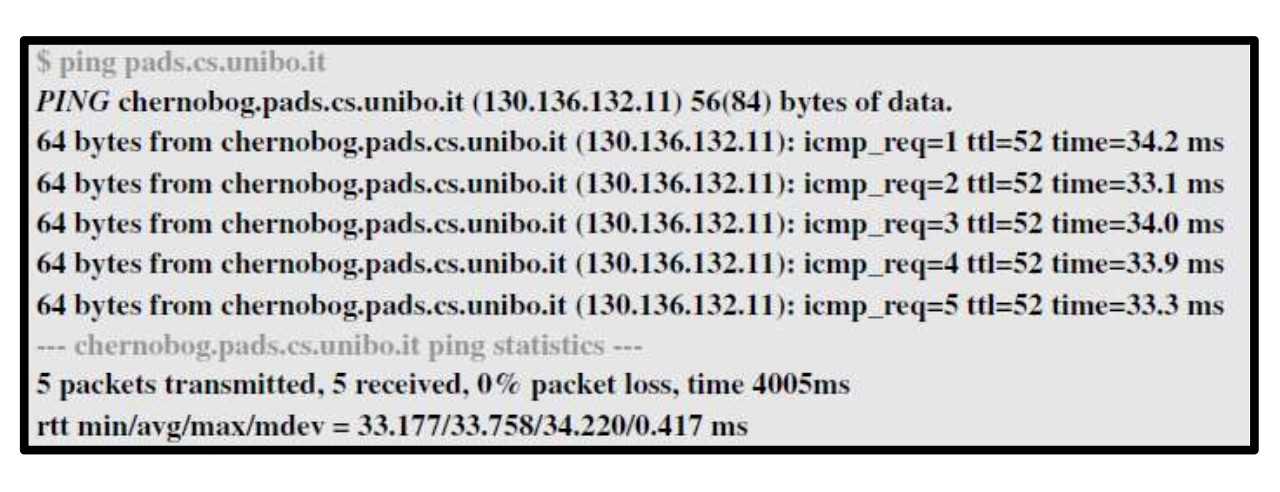
\includegraphics[width=0.8\textwidth]{immagini/Ping.jpg}
    \caption*{Invio di un messaggio ping al sito pads.cs.unibo.it}
\end{figure}

\paragraph{Traceroute}

Il programma \emph{traceroute} in UNIX o \emph{tracert} in Windows può essere utilizzato per individuare il percorso di un datagramma dalla sorgente alla destinazione tramite l’identificazione dell’indirizzo IP di tutti i router che vengono visitati lungo il percorso.\
Solitamente il programma viene impostato per un massimo di 30 salti (router), che sono usualmente sufficienti per raggiungere la destinazione.

Il programma \emph{traceroute} ha un funzionamento molto diverso da \emph{ping}.\
\emph{Ping} è basato su due messaggi query; \emph{traceroute} è invece implementato per mezzo di due messaggi di segnalazione degli errori:\ tempo scaduto e porta destinazione non raggiungibile.

\begin{figure}[H]
    \centering
    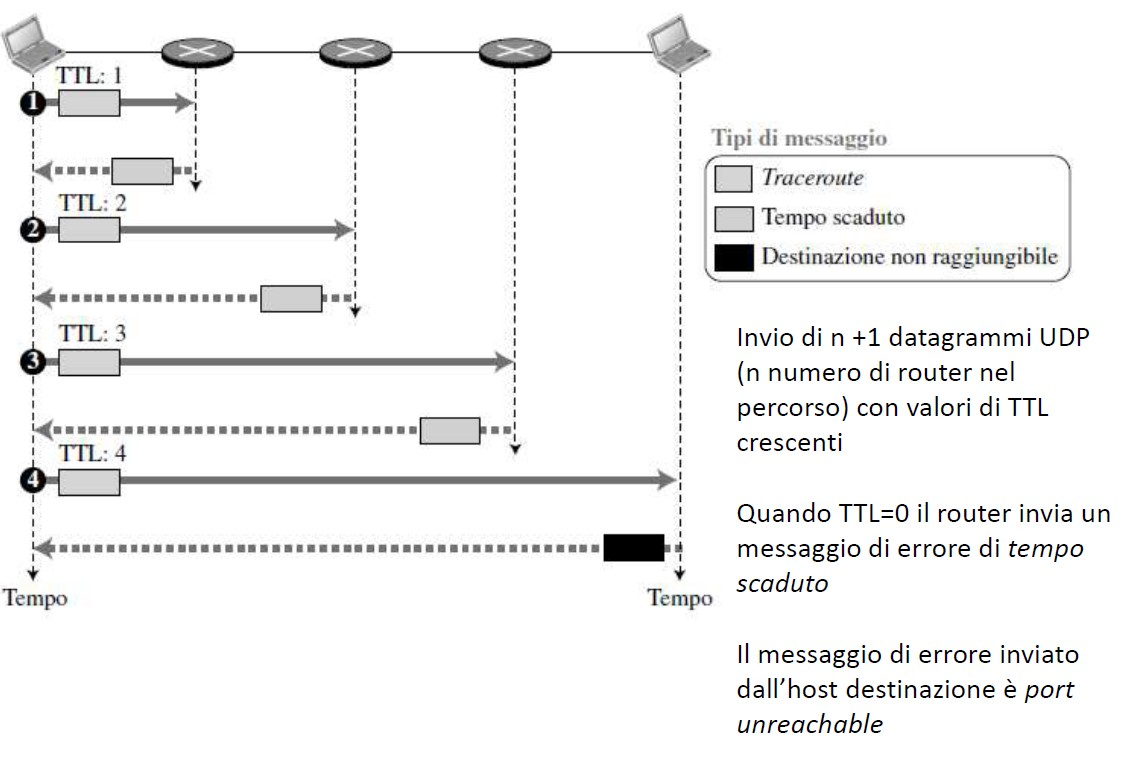
\includegraphics[width=0.9\textwidth]{immagini/Traceroute.jpg}
    \caption*{Esempio di funzionamento del programma traceroute}
\end{figure}

Il programma \emph{traceroute} imposta inoltre un timer per trovare il tempo di round-trip di ciascun router e della destinazione.\
La maggior parte dei programmi \emph{traceroute} invia tre messaggi a ogni dispositivo, con lo stesso valore di TTL, per poter effettuare una stima migliore del tempo di round-trip.\
Quanto segue mostra un esempio di funzionamento del programma \emph{traceroute} che utilizza tre messaggi per ogni dispositivo e ottiene quindi tre RTT.

\begin{figure}[H]
    \centering
    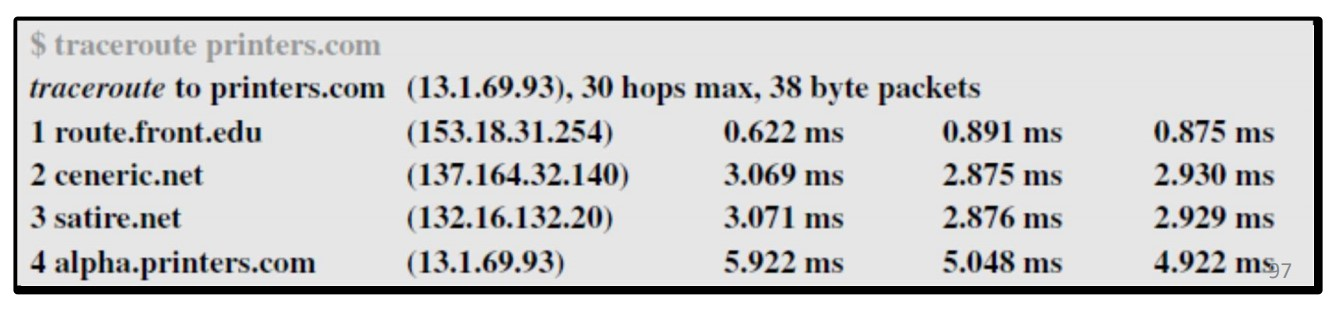
\includegraphics[width=0.9\textwidth]{immagini/Traceroute_RTT.jpg}
\end{figure}

\section{Architettura di un Router}

\begin{table}[H]
    \centering
    \begin{tabular}{m{15em}|m{15em}}
        \textbf{\emph{Forwarding (inoltro)}}                           & \textbf{\emph{Routing (instradamento)}}                                                        \\
        \hline
        Trasferire i pacchetti sull'appropriato collegamento in uscita & Processo decisionale di scelta del percorso verso una destinazione                             \\
        \hline
        Usa la tabella d'inoltro                                       & Determina i valori da inserire nella tabella d'inoltro tramite gli algoritmi di \emph{routing} \\
        \hline
        Avviene al livello del piano di dati                           & Avviene al livello del piano di controllo                                                      \\
    \end{tabular}
\end{table}

\begin{figure}[H]
    \centering
    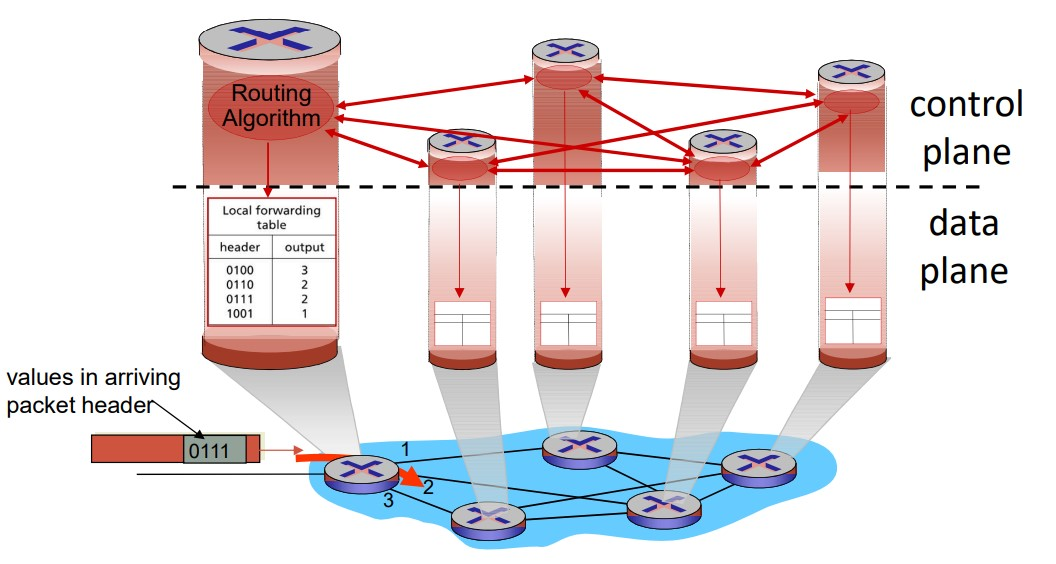
\includegraphics[width=\textwidth]{immagini/Router_decentralizzato.jpg}
    \captionsetup{singlelinecheck=off}
    \caption*{\centering
        Routing decentralizzato:\
        \begin{itemize}
            \item Algoritmo di routing in esecuzione su ciascun router
            \item I router si scambiano messaggi (protocolli di routing)
        \end{itemize}}
\end{figure}
\begin{figure}[H]
    \centering
    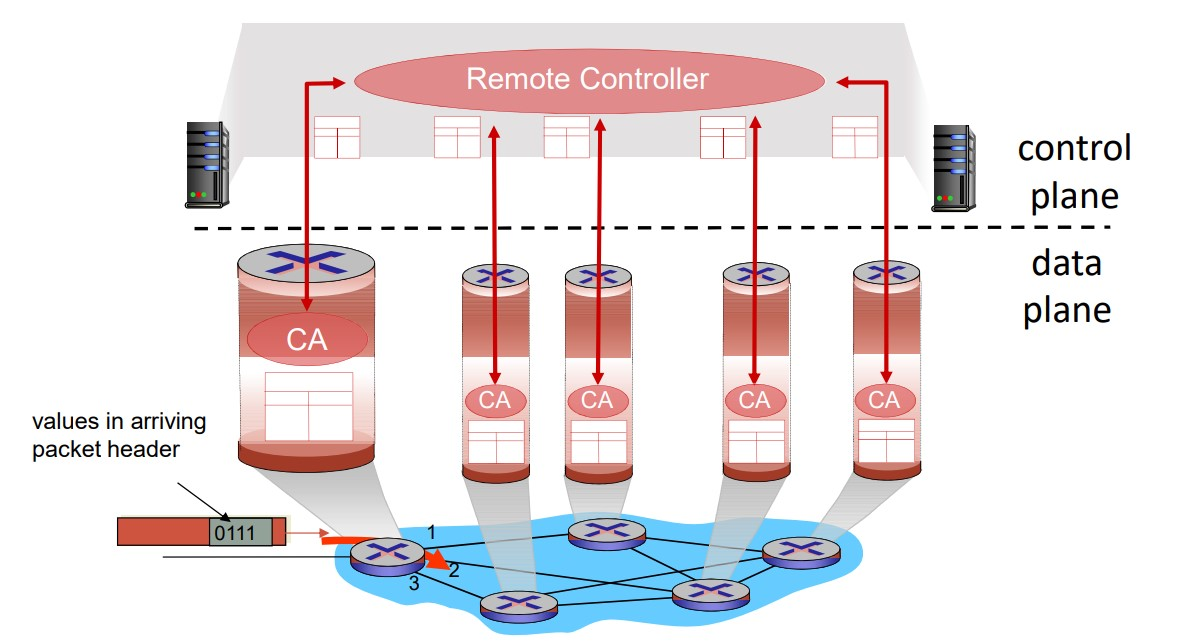
\includegraphics[width=\textwidth]{immagini/Routing_centralizzato.jpg}
    \captionsetup{singlelinecheck=off}
    \caption*{\centering Routing logicamente centralizzato (\emph{Software-defined Networking (SDN)})

        Un controller remoto interagisce con Control Agents locali:

        \begin{itemize}
            \item Riceve dai CA informazioni sui collegamenti e sul traffico
            \item Invia ai CA i valori da inserire nella tabella di inoltro
        \end{itemize}}
\end{figure}

Nella nostra discussione circa l’inoltro e l’instradamento abbiamo rappresentato il router come una scatola nera che accetta pacchetti in entrata da una delle porte di input (interfacce), usa una tabella d’inoltro per trovare la porta di output e da questa invia il pacchetto.\

\begin{figure}[H]
    \centering
    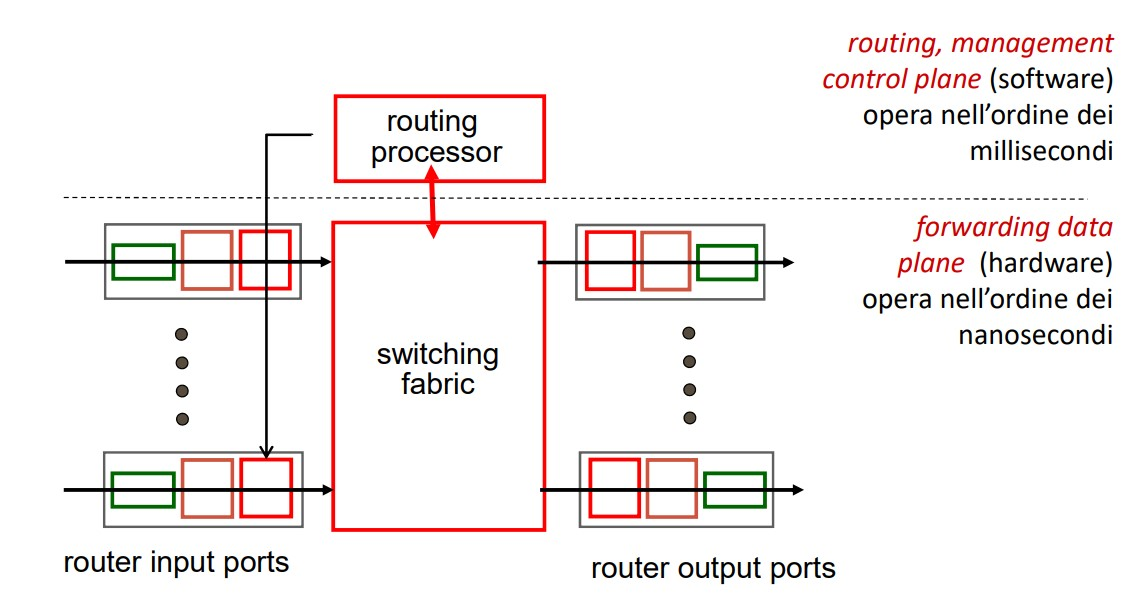
\includegraphics[width=0.8\textwidth]{immagini/Architettura_router.jpg}
    \caption*{Componenti di un router}
\end{figure}

\subsubsection{Porte di input}

\begin{figure}[H]
    \centering
    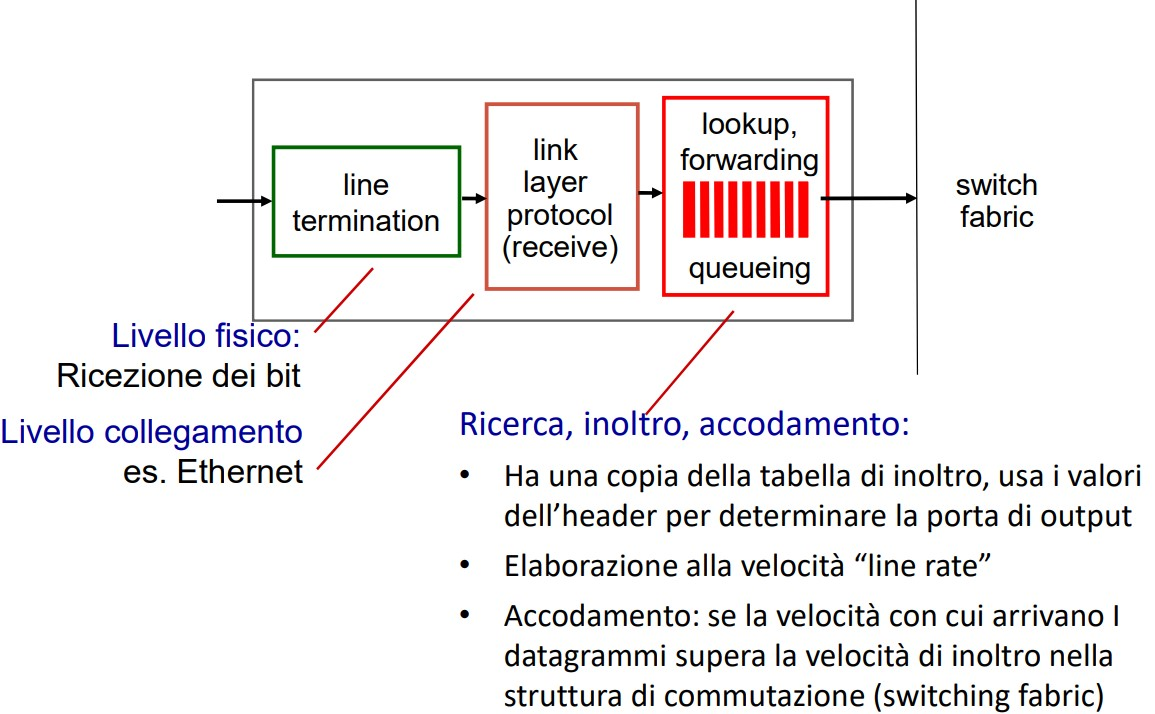
\includegraphics[width=0.8\textwidth]{immagini/PorteInput.jpg}
    \caption*{Porte di input}
\end{figure}

\subsubsection{Switching fabric (struttura di commutazione)}

\begin{figure}[H]
    \centering
    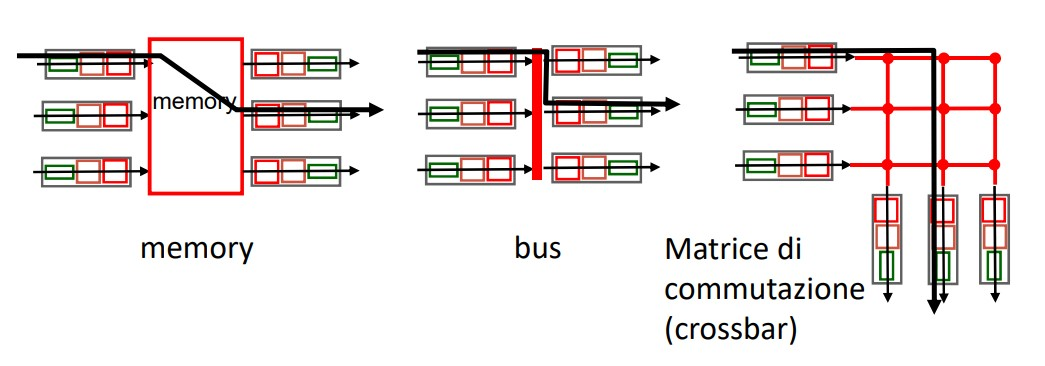
\includegraphics[width=0.8\textwidth]{immagini/Switching.jpg}
    \caption*{Switching fabric}
\end{figure}
\begin{itemize}
    \item Trasferisce il pacchetto dal buffer di input al buffer di output appropriato
    \item Velocità di commutazione:\ velocità con cui i pacchetti possono essere trasferiti dagli ingressi alle uscite
          \begin{itemize}
              \item N input:\ velocità di commutazione auspicabile N volte la velocità di linea
          \end{itemize}
\end{itemize}

\subsubsection{Porte di output}

\begin{figure}[H]
    \centering
    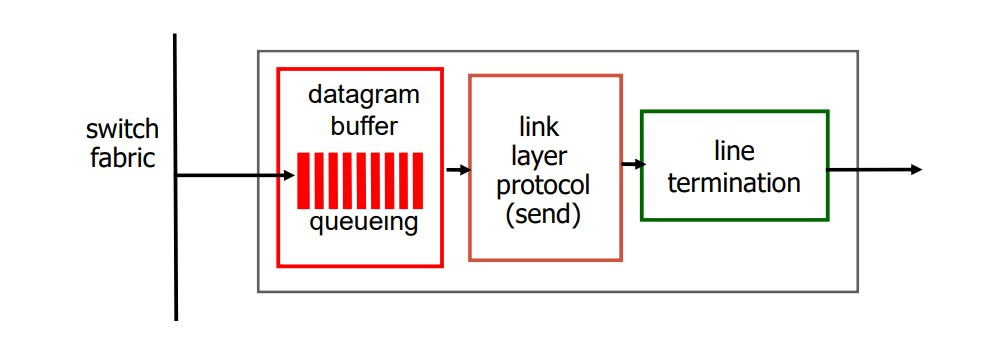
\includegraphics[width=0.8\textwidth]{immagini/PorteOutput.jpg}
    \caption*{Porte di output}
\end{figure}
\begin{itemize}
    \item \textbf{\emph{Buffering}} richiesto quando i datagrammi arrivano dalla struttura di commutazione ad una velocità maggiore della velocità di trasmissione sul collegamento in uscita
    \item \textbf{\emph{Scheduling}}:\ politiche per definire l’ordine di trasmissione dei datagrammi
\end{itemize}

\section{Routing unicast}

In una rete come Internet lo scopo del livello di rete è quello di consegnare un datagramma dalla sorgente alla destinazione o alle destinazioni.\
Se un datagramma è destinato ad una sola destinazione (consegna uno-a-uno) si parla di \emph{routing unicast}.\
Se il datagramma è destinato a numerose destinazioni (consegna uno-a-molti) si parla di \emph{routing multicast}.\
Infine, se il datagramma deve essere consegnato a tutti gli host della rete (uno-a-tutti), si parla di \emph{routing broadcast}.

\subsection{Concetti generali}

Nel routing unicast un pacchetto viene instradato, salto dopo salto, dalla sua sorgente alla sua destinazione con l'aiuto delle tabelle d'inoltro.\
L'host sorgente non ha bisogno di alcuna tabella d'inoltro visto che si limita a consegnare il proprio pacchetto al router di default della sua rete locale.\
Neanche l'host di destinazione ha bisogno di una tabella d'inoltro, poiché riceve il pacchetto direttamente dal router di default della sua rete locale.\
Questo significa che solo i router che collegano tra loro le diverse reti hanno bisogno di tabelle d'inoltro.\
Instradare un pacchetto dalla sua sorgente alla sua destinazione significa pertanto instradare il pacchetto da un \emph{router sorgente} (il router di default dell'host sorgente) a un \emph{router di destinazione} (il router collegato alla rete di destinazione ).\
Anche se un pacchetto deve passare attraverso i router sorgente e destinazione, la domanda è:\ quali altri router dovrà attraversare il pacchetto? In altre parole, poiché solitamente ci sono molti percorsi diversi tra sorgente e la destinazione, quale percorso dovrà effettuare il pacchetto?

Per trovare il percorso migliore, una rete di reti (ovvero una internet) può essere modellata per mezzo di un \emph{grafo}.\
Un grafo in informatica è formato da un insieme di \emph{nodi} collegati da \emph{archi}.\
Per modellare una internet per mezzo di un grafo, possiamo pensare che ogni router sia un nodo ed ogni rete, tra una coppia di router, sia un arco.\
Una internet, infatti, è modellata come un \emph{grafo pesato}, in cui ad ogni arco è associato un costo.\
Se viene usato un grafo pesato per rappresentare un'area geografica, i nodi possono essere le città e gli archi le strade che le collegano; i pesi, in questo caso, sono le distanze tra le città.\
Nell'instradamento, tuttavia, il costo di un arco ha un'interpretazione diversa a seconda dei diversi protocolli di routing.\
Per il momento supponiamo che ci sia un costo associato ad ogni arco.\
Se non c'è un arco che collega due nodi allora il costo associato è infinito.

\begin{figure}[H]
    \centering
    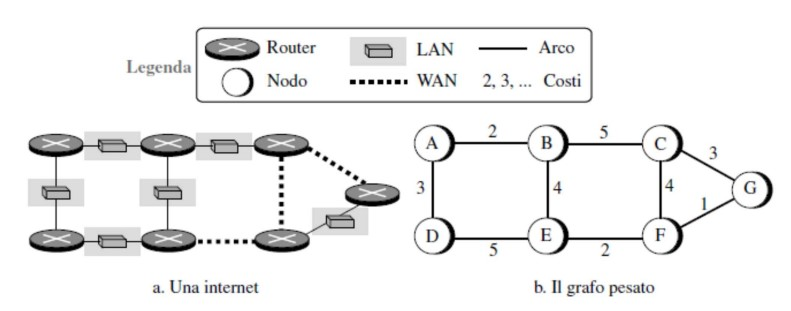
\includegraphics[width=0.8\textwidth]{immagini/Rete_grafo.jpg}
    \caption*{Una rete e la sua rappresentazione sotto forma di grafo}
\end{figure}

\subsubsection{\emph{Instradamento a costo minimo}}

Quando una internet viene rappresentata come un grafo pesato, uno dei modi per interpretare il percorso \emph{migliore} dal router sorgente al router destinazione è trovare il \emph{minor costo} tra i due.\
In altre parole il router sorgente sceglie il percorso verso il router destinazione in modo che il costo totale del percorso sia il costo minimo tra tutti i percorsi possibili.\
Nella figura il percorso migliore tra A ed E è A-B-E, con costo 6.\
Ciò significa che, per poter instradare i pacchetti utilizzando questa metrica, ogni router deve trovare il percorso a costo minimo tra se stesso e tutti gli altri router.

\subsubsection{\emph{Alberi di costo minimo}}

Se in una rete ci sono \emph{N} router allora ci sono ($N-1$) percorsi a costo minimo da ogni router a ogni altro router.\
Ciò significa che servono $N \cdot (N-1)$ percorsi a costo minimo per l'intera rete.\
Quindi, in una rete con solo 10 router ci sono 90 percorsi a costo minimo.\
Un modo migliore per vedere tutti questi percorsi è combinarli in un \emph{albero di costo minimo}.\
Un albero di costo minimo è un albero con il router sorgente che fa da radice e che visita tutti gli altri nodi dell'albero seguendo sempre il percorso più corto (meno costoso) tra quelli possibili.\
In questo modo possiamo avere un solo albero di costo minimo per ogni nodo; avremo quindi \emph{N} alberi di costo minimo per l'intera rete.

\subsection{Algoritmi di routing}

\subsubsection{Routing statico e dinamico}

\begin{itemize}
    \item Nel \textbf{routing statico} le righe (entry) della tabella vengono configurate manualmente dall’operatore.\
          Tale metodo viene usato per reti di piccole dimensioni e la cui topologia non varia molto, dove è possibile prevedere tutti i possibili percorsi di un pacchetto IP nella rete.
    \item Nel \textbf{routing dinamico} esistono protocolli specifici che provvedono automaticamente ad inserire nella tabella del router le entry relative ai possibili percorsi.\
          Viene usato nelle reti di medie-grandi dimensioni e con topologia variabile (grandi reti locali private e Internet).
\end{itemize}

\subsubsection{Algoritmi di instradamento globali/decentralizzati}

Gli algoritmi di instradamento si possono classificare in:
\begin{itemize}
    \item \textbf{Globali}, se si basano sulla conoscenza della topologia di tutta la rete.\
          Il calcolo può essere fatto in un unico sito (algoritmo centralizzato) o in più nodi, utilizzando informazioni sulla connettività di tutti i nodi e sui costi di tutti i link (es.\ algoritmo \textbf{Link State}).
          \begin{itemize}
              \item L’algoritmo riceve in ingresso informazioni su tutti i collegamenti tra i nodi e i loro costi.
          \end{itemize}
    \item \textbf{Decentralizzati}, quando nessun nodo conosce la topologia di tutta la rete, ma ha informazioni solo sui nodi e link vicini.\
          Il calcolo del percorso è iterativo e distribuito (es.\ algoritmo \textbf{Distance Vector}).
          \begin{itemize}
              \item Ogni nodo elabora un vettore di stima dei costi (distanze) verso tutti gli altri nodi nella rete.
              \item Il cammino a costo minimo viene calcolato in modo distribuito e iterativo scambiandosi informazioni con i nodi vicini.
          \end{itemize}

\end{itemize}

\subsubsection{\emph{Routing basato su vettore distanza}}

Nel distance-vector routing, per prima cosa ogni nodo crea il proprio albero di costo minimo con le informazioni di base che possiede sui suoi soli nodi vicini.\
Il risultato sono degli alberi incompleti (mancano tutte le informazioni dei nodi che non sono vicini).\
Questi alberi incompleti vengono a questo punto scambiati tra i vicini per rendere l'albero sempre più completo e rappresentare così l'intera rete.\
Nel distance-vector routing quello che accade è che ogni router comunica continuamente a tutti i suoi vicini ciò che sa sulla rete (anche se, ovviamente, potrebbe non sapere tutto).

\paragraph{\emph{Equazione di Bellman-Ford}}

Il fulcro del routing basato su vettore distanza è la famosa equazione di \emph{Bellman-Ford}.\
Questa equazione viene usata per trovare il costo minimo (distanza minima) tra un nodo sorgente, \emph{x}, e un nodo destinazione, \emph{y}, tramite dei nodi intermedi (\textbf{a}, \textbf{b}, \textbf{c}, \dots) dove i costi tra il nodo sorgente e i nodi intermedi e i costi minimi tra i nodi intermedi e la destinazione sono noti.\
Di seguito mostriamo il caso generale in cui D\textsubscript{ij} è la distanza minima e c\textsubscript{ij} è il costo tra il nodo \textbf{\emph{i}} e il nodo \textbf{\emph{j}}.
\begin{center}
    $D_{xy} = \min\{(c_{xa}+D_{ay}), (c_{xb}+D_{by}), (c_{xc}+D_{cy}), \dots\}$
\end{center}
Nel distance-vector routing, quello che si vuole fare normalmente è aggiornare un costo minimo esistente con il costo minimo che si ottiene passando attraverso un nodo intermedio, come ad esempio \emph{z}, se quest'ultimo è minore.\
In questo caso l'equazione diventa più semplice.
\begin{center}
    $D_{xy} = \min\{D_{xy}, (c_{xz}+D_{zy})\}$
\end{center}
Possiamo dire che l'equazione di Bellman-Ford ci permette di costruire un nuovo percorso a costo minimo rispetto ai percorsi a costo minimo precedentemente stabiliti.

\paragraph{\emph{Vettori distanza}}

Il concetto di \emph{vettore distanza} è alla base del distance-vector routing.\
Un albero a costo minimo è una combinazione di percorsi a costo minimo dalla radice dell'albero verso tutte le destinazioni.\
Tali percorsi vengono collegati insieme per formare l'albero.\
Il routing a vettore distanza scinde questi percorsi e crea quello che viene chiamato un \emph{vettore distanza}, cioè un array monodimensionale che rappresenta l'albero.\

Da notare che il ``\emph{nome}'' del vettore distanza definisce la radice, gli \emph{indici} invece definiscono le destinazioni e il \emph{valore} di ogni cella definisce il costo minimo dalla radice alla destinazione.\
Un vettore distanza non fornisce il percorso da seguire per giungere alla destinazione (informazione che invece l'albero è in grado di fornire); il vettore riporta solo i costi minimi per le destinazioni.

Sappiamo che un vettore distanza può rappresentare i percorsi a costo minimo di un albero a costo minimo, ma la questione è:\ in quale modo i nodi all'interno di una rete all'inizio creano il proprio vettore distanza? Ogni nodo della rete, quando viene inizializzato, crea un vettore distanza molto rudimentale con le sole informazioni che il nodo riesce ad ottenere dai propri vicini (i nodi con cui è direttamente collegato).\
Per far questo, il nodo invia alcuni messaggi di benvenuto attraverso tutte le sue interfacce e scopre l'identità dei vicini e la sua distanza con ciascuno di essi.\
Quindi crea un semplice vettore distanza inserendo la distanze scoperte nelle celle corrispondenti e lascia il valore delle altre celle ad infinito.\
Questi vettori rappresentano i percorsi a costo minimo elaborati sulla base delle solo informazioni (limitate) di cui dispone il nodo in questo momento.\
Quando si è a conoscenza di una sola distanza tra due nodi, questa può essere considerata il minimo.\
La Figura \ref{Vettori} mostra tutti i vettori distanza per la nostra rete.\
È bene notare che non c'è alcuna necessità che i vettori siano costruiti in modo sincrono, ogni nodo può essere inizializzato in modo del tutto indipendente (asincrono) dagli altri.

\begin{figure}[H]
    \centering
    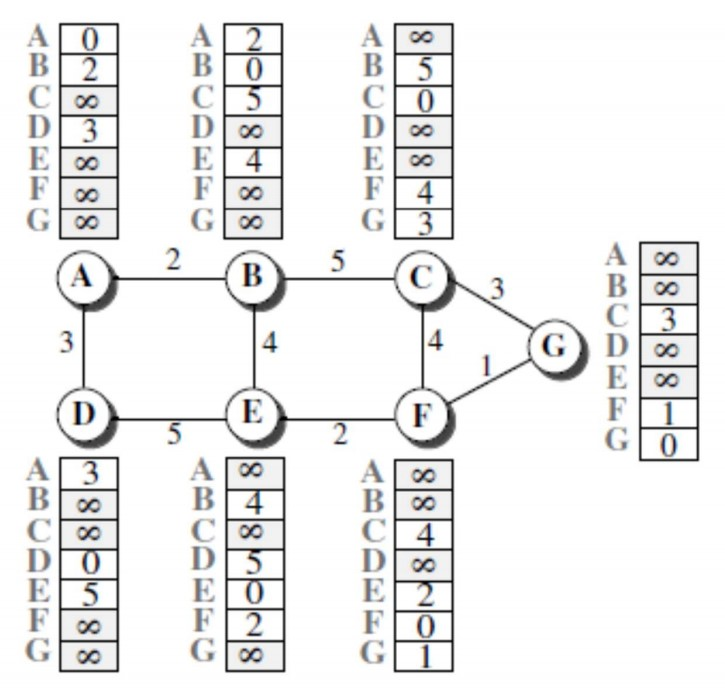
\includegraphics[width=0.5\textwidth]{immagini/Vettori_distanza.jpg}
    \caption{Vettori iniziali dei nodi di una rete}
    \label{Vettori}
\end{figure}
Questi vettori rudimentali non permettono veramente ad una rete di inoltrare i pacchetti.\
Per esempio il nodo A crede di non essere collegato al nodo G in quanto la cella corrispondente mostra un costo infinito.\
Dopo che ogni nodo ha creato il suo vettore ne invia una copia a tutti i suoi vicini.\
Quando un nodo riceve un vettore distanza da un vicino provvede ad aggiornare il suo vettore distanza applicando l'equazione Bellman-Ford (seconda versione).\
Tuttavia bisogna aggiornare non solo un costo minimo ma \emph{N} costi minimi, dove \emph{N} è il numero di nodi nella rete.\
Se stiamo usando un programma, possiamo farlo con una semplice iterazione; se invece stiamo lavorando su carta, possiamo mostare l'intero vettore invece delle \emph{N} equazioni separate.
\begin{figure}[H]
    \centering
    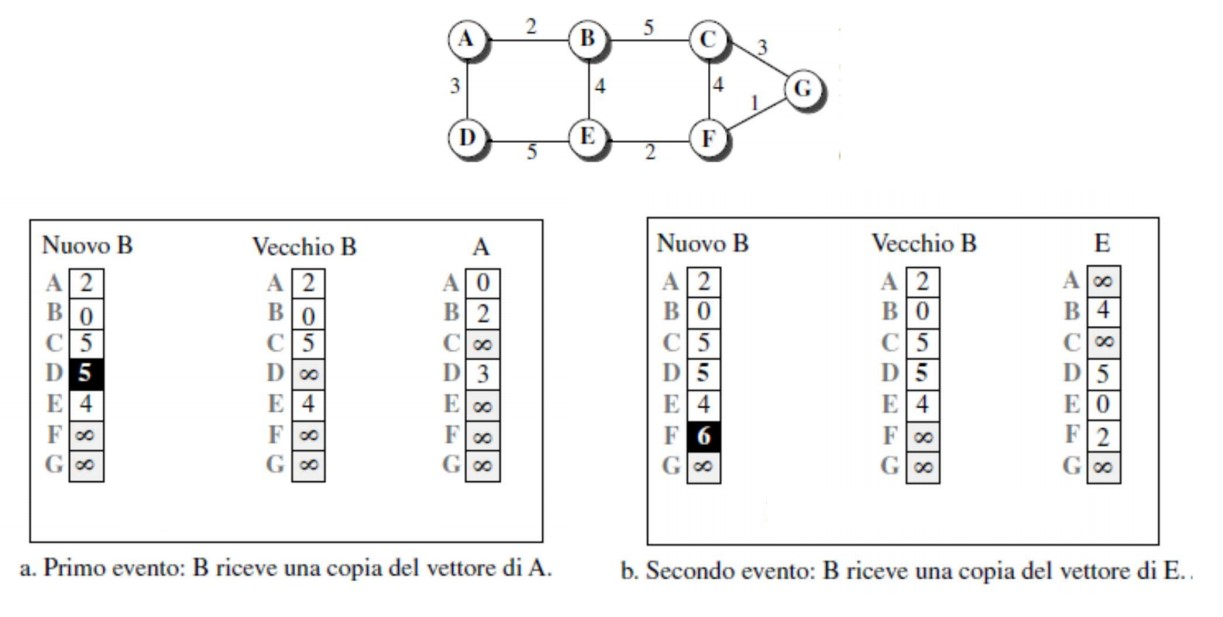
\includegraphics[width=\textwidth]{immagini/Aggiornamento_vettore_distanza.jpg}
    \caption {Aggiornamento dei vettori distanza}
    \label{aggiornamento}
\end{figure}
Ed è esattamente quanto riportiamo nella Figura \ref{aggiornamento}.\
La figura mostra due eventi asincroni, che avvengono uno dopo l'altro, a distanza di qualche tempo.\
Nel primo evento il nodo A ha inviato il suo vettore al nodo B.\
Il nodo B aggiorna il suo vettore usando il costo $c_{BA} = 2$.\
Nel secondo evento E ha mandato il suo vettore al nodo B.\
Il nodo B aggiorna il suo vettore usando il costo $c_{EA} = 4$.

Grazie al primo evento, il nodo B ha un miglioramento nel suo vettore:\ il suo costo minimo verso il nodo D è ora cambiato da infinito a 5 (passando attraverso il nodo A).\
Dopo il secondo evento il nodo B ha un ulteriore miglioramento del suo vettore:\ il suo costo minimo verso il nodo F è cambiato da infinito a 6 (passando attraverso il nodo E).

Dopo l'aggiornamento di un nodo, esso invia immediatamente il suo vettore aggiornato a tutti i vicini.\
Anche se i suoi vicini hanno ricevuto il vettore precedente, quello aggiornato può portare a dei miglioramenti.

\paragraph{\emph{Algoritmo di routing basato su vettore distanza}}

Finalmente possiamo vedere lo pseudocodice semplificato che descrive l'algoritmo di routing basato su vettore di distanza.\
L'algoritmo viene eseguito da ogni nodo in modo indipendente e asincrono.
\begin{figure}[H]
    \centering
    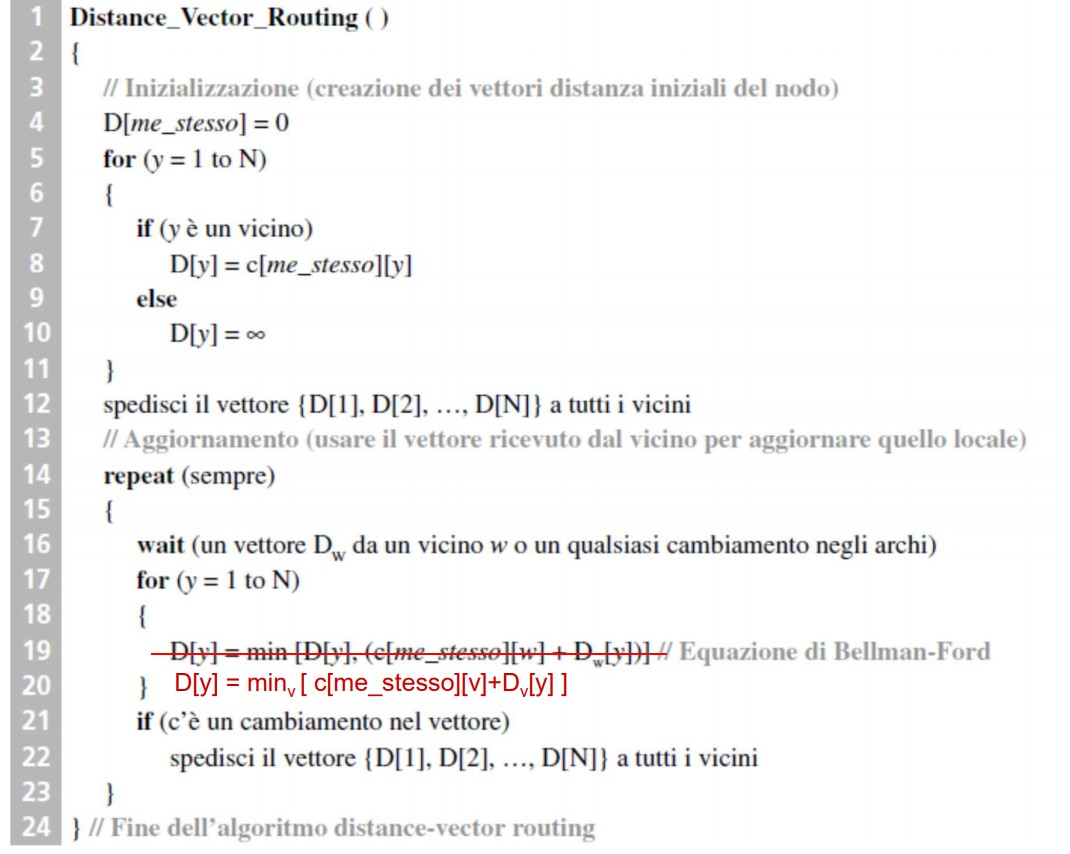
\includegraphics[width=0.8\textwidth]{immagini/Algoritmo_vectorDIstance.jpg}
    \caption*{Algoritmo del distance-vector routing}
\end{figure}
Le righe da 4 a 11 inizializzano il vettore locale del nodo.\
Le righe da 14 a 23 mostrano come il vettore venga aggiornato dopo aver ricevuto un nuovo vettore da un vicino.\
Il ciclo \emph{for} (nelle righe da 17 a 20) si occupa di aggiornare tutte le celle del vettore locale in base agli aggiornamenti contenuti nel nuovo vettore che è stato ricevuto.\
Da notare che il nodo invia il suo vettore due volte:\ alla riga 12 subito dopo l'inizializzazione e alla riga 22 dopo ogni aggiornamento.

\paragraph{\emph{Conteggio all'infinito}}

Un problema con il routing basato sul vettore distanza è che i decrementi di costo (cioè le buone notizie) si diffondono rapidamente, mentre gli aumenti di costo (le cattive notizie) si propagano lentamente.\
Affinché un protocollo di routing lavori correttamente, se un collegamento è rotto (e quindi il costo del relativo arco diventa infinito), ogni altro router dovrebbe venirne a conoscenza immediatamente, ma nel routing basato su vettore distanza serve avere un po' di tempo.\
Questo problema è spesso chiamato \emph{conteggio all'infinito}.\
A volte servono molti aggiornamenti prima che il costo di un collegamento rotto venga registrato come infinito da tutti i router.

\paragraph{\emph{Ciclo a due nodi}}

Un esempio di conteggio all'infinito è il problema del ciclo a due nodi.\
Per comprendere il problema, diamo un'occhiata allo scenario illustrato nella Figura \ref{Infinity_count}.

\begin{figure}[H]
    \centering
    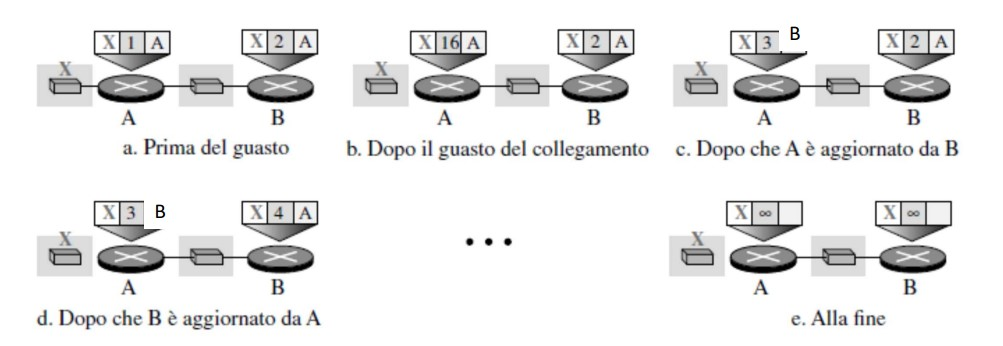
\includegraphics[width=\textwidth]{immagini/Infinity_count.jpg}
    \caption{Instabilità a due nodi}
    \label{Infinity_count}
\end{figure}
La figura illustra un sistema formato da tre nodi.\
Abbiamo mostrato solo le parti della tabella d'inoltro necessarie per la discussione.\
All'inizio sia il nodo A che il nodo B sanno come raggiungere il nodo X.\
Ma improvvisamente si guasta il collegamento tra A e X.\
Di conseguenza, il nodo A modifica la sua tabella.\
Se A invia immediatamente la sua tabella a B non c'è alcun problema.\
Tuttavia, se B invia la sua tabella d'inoltro ad A prima di ricevere quella di A, il sistema diventa instabile.\
Il nodo A riceve l'aggiornamento e, supponendo che B abbia trovato un modo per raggiungere X, aggiorna immediatamente la sua tabella d'inoltro.\
Ora A invia il suo nuovo aggiornamento a B.\
Quello che accade è che B è portato a credere che qualcosa sia cambiato vicino ad A e di conseguenza aggiorna la sua tabella d'inoltro.\
Il costo per raggiungere X aumenta gradualmente fino ad arrivare all'infinito.\
Ora, finalmente, sia A che B sanno che X non può essere raggiunto.\
Tuttavia, durante questo periodo di tempo il sistema non è stabile.\
Il nodo A crede che il percorso per raggiungere X passi da B e il nodo B crede che il percorso per raggiungere X passi attraverso A.\
Se A riceve un pacchetto destinato X il pacchetto va a B e quindi ritorna ad A.\
Allo stesso modo, se B riceve un pacchetto destinato ad X, va verso A e torna a B.\
I pacchetti rimbalzano tra A e B, creando un ciclo a due nodi.\
Di seguito vengono illustrate alcune soluzioni proposte per risolvere i problema d'instabilità di questo tipo.

\paragraph{\emph{Split horizon (orizzonte spaccato)}}

Una soluzione all'instabilità viene chiamata \emph{split horizon}.\
Con questa strategia invece di inviare la tabella attraverso ogni interfaccia, ciascun nodo invia solo una parte della sua tabella tramite le sue varie interfacce.\
Se, secondo tale tabella, il nodo B ritiene che il percorso ottimale per raggiungere X passi tramite A, allora non deve fornire questa informazione ad A:\ l'informazione è arrivata ad A che quindi la conosce già.\
Il fatto che le informazioni vengano prese dal nodo A, vengano modificate e inviate nuovamente al nodo A è ciò che crea confusione.\
Nel nostro scenario, il nodo B elimina l'ultima riga della sua tabella d'inoltro prima di inviarla ad A.\
In questo caso il nodo A mantiene il valore di infinito come distanza verso X.\
Più tardi, quando il nodo A invia la sua tabella d'inoltro a B, anche il nodo B corregge la sua tabella.\
Il sistema diventa stabile dopo il primo aggiornamento:\ sia il nodo A che il nodo B sanno che X non è più raggiungibile.

\paragraph{\emph{Poisoned reverse (inversione avvelenata)}} L'utilizzo della strategia split horizon ha un effetto collaterale.\

Normalmente il protocollo che implementa l'algoritmo di routing utilizza un timer:\ se per una certa quantità di tempo non ci sono novità circa un percorso, il nodo lo elimina dalla sua tabella.\
Quando il nodo B, nello scenario precedente, elimina il percorso verso X dai suoi annunci ad A, il nodo A non può sapere se ciò è dovuto alla strategia split horizon (la sorgente delle informazioni era A) o se dipende dal fatto che B recentemente non ha ricevuto alcuna notizia di X.\
Nella strategia di inversione avvelenata, B può ancora rendere pubblico il valore per X, ma se la sorgente delle informazioni è A, allora sostituisce la distanza con valore infinito.\
In questo caso l'infinito viene usato come avvertimento:\ ``Non usare questo valore, quello che so circa questo percorso viene da te''.

\paragraph{\emph{Instabilità a tre nodi}}

L'instabilità a due nodi si può evitare utilizzando la strategia split horizon combinata all'inversione avvelenata.\
Tuttavia, se l'instabilità è a tre nodi, la stabilità non può essere garantita.

\subsubsection{\emph{Routing a stato del collegamento}}

Un algoritmo di routing che deriva direttamente dalla nostra precedente discussione sulla creazione degli alberi a costo minimo e delle tabelle d'inoltro è il \emph{routing a stato del collegamento}, \emph{Link-State (LS) routing}.

Questo metodo utilizza il termine \emph{link-state} (stato del collegamento) per definire le caratteristiche di un collegamento (un arco) che rappresenta una rete, parte di una internet.\
In questo algoritmo, il costo associato ad un arco definisce lo stato del collegamento.\
I collegamenti con costi inferiori sono preferibili rispetto a quelli con costi superiori; se il costo di un collegamento è infinito, significa che esso non esiste più o è stato interrotto.

\paragraph{\emph{Link-State Database (LSDB)}}

Per creare un albero a costo minimo utilizzando questo metodo ogni nodo deve avere un \emph{mappa} completa della rete, il che significa che deve conoscere lo stato di ciascun collegamento.\
La raccolta di stati per tutti i collegamenti viene chiamata \emph{Link-State Database (LSDB)}.\
Il LSDB è unico per l'intera rete, ma ogni nodo deve averne un duplicato per poter essere in grado di creare l'albero di costo minimo.\
Il LSDB può essere rappresentato per mezzo di un array bidimensionale (matrice) in cui il valore di ogni cella definisce il costo del collegamento corrispondente.

\begin{figure}[H]
    \centering
    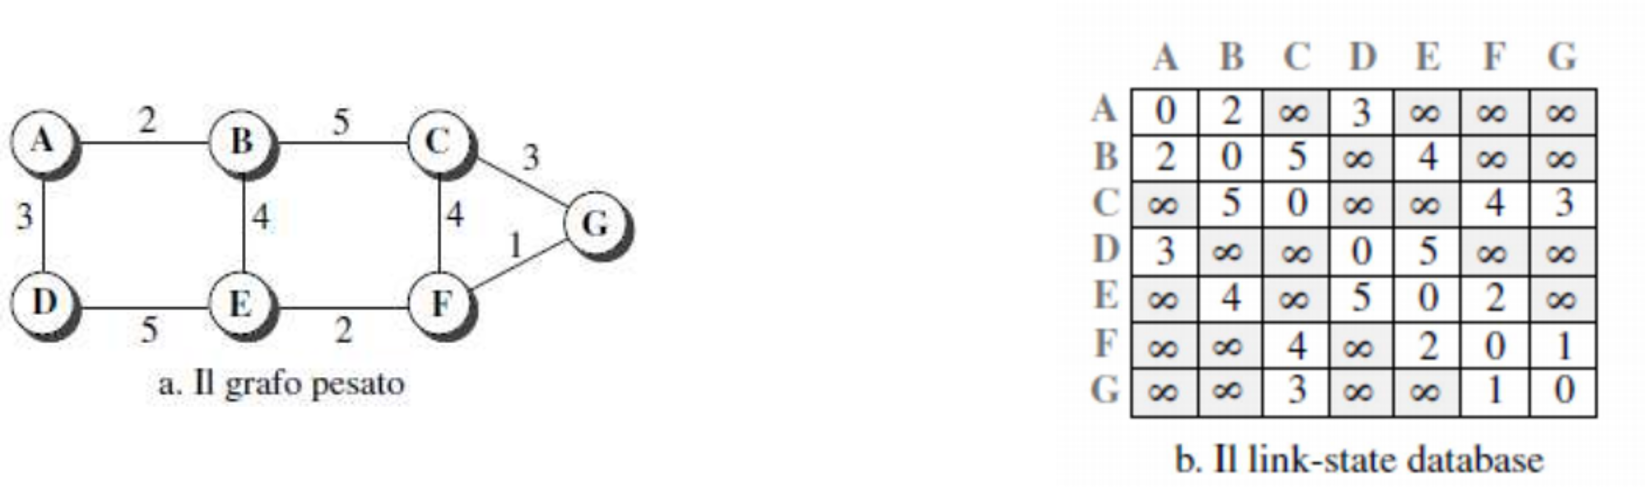
\includegraphics[width=\textwidth]{immagini/LSDB.png}
    \caption*{Esempio di un link-state database}
\end{figure}

Ora il problema è:\ come può ogni nodo creare la sua copia del LSDB che contenga le informazioni necessarie sull'intera rete? Ciò può essere fatto tramite un procedimento chiamato \emph{flooding} (inondazione).\
Ogni nodo può inviare dei messaggi di benvenuto a tutti i suoi vicini (i nodi ai quali è collegato direttamente) per raccogliere una coppia di informazioni circa ogni suo vicino:\ l'identità del nodo e il costo del collegamento.\
La combinazione di queste due informazioni viene chiamata \emph{pacchetto LS} (LS packet, LSP).\
L'LSP viene inviato attraverso ogni interfaccia del nodo.
\begin{figure}[H]
    \centering
    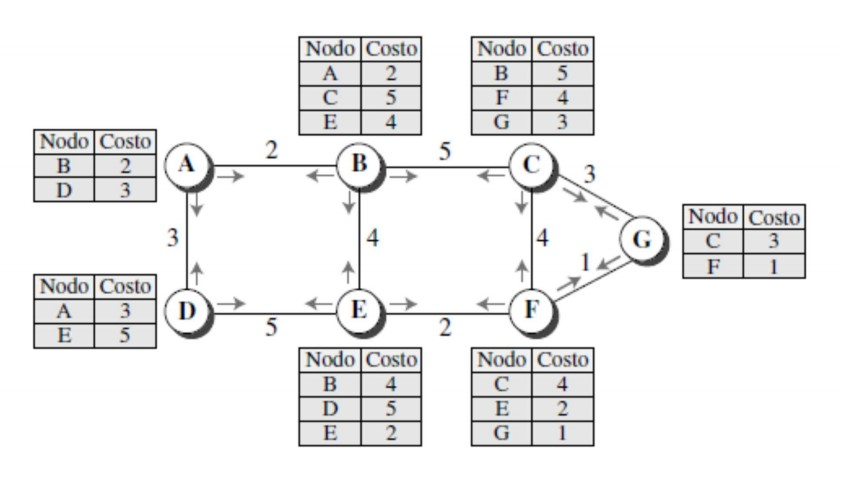
\includegraphics[width=0.8\textwidth]{immagini/LSPacket.jpg}
    \caption*{Gli LSP creati ed inviati da ciascun nodo per costruire l'LSDB}
\end{figure}
Quando un nodo riceve l'LSP da una delle sue interfacce, confronta il nuovo LSP con un'eventuale vecchia copia che potrebbe già avere.\
Se l'LSP appena arrivato è più vecchio di quello che ha già (e questo è rilevabile confrontando i numeri di sequenza), l'LSP viene scartato.\
Se è più recente o è il primo ricevuto, il nodo scarta il vecchio LSP (se ce n'è uno) e conserva quello che ha appena ricevuto.\
A questo punto il nodo invia una copia dell'LSP da ogni sua interfaccia ad esclusione di quella da cui è arrivato il pacchetto.\
Questo garantisce che il flooding si interrompa da qualche parte nella rete (ad esempio dove un nodo ha una sola interfaccia).\
Dopo aver ricevuto tutti i nuovi LSP, ogni nodo è in grado di creare la sua copia dell'LSDB globale.\
Questo LSDB è esattamente uguale per ogni nodo e rappresenta l'intera mappa della rete.

A questo punto possiamo confrontare l'algoritmo di routing a stato del collegamento con quello a vettore distanza.\
In quest'ultimo, ogni router comunica ai suoi vicini ciò che sa sull'intera rete, mentre nell'algoritmo di routing a stato del collegamento ogni router riferisce all'intera rete ciò che sa dei vicini.

\paragraph{\emph{Costruzione degli alberi a costo minimo}}

Per costruire il suo albero a costo minimo utilizzando l'LSDB condiviso, ogni nodo deve eseguire il famoso \emph{algoritmo di Dijkstra}.\
Questo algoritmo iterativo è composto dai seguenti passi:

\begin{enumerate}
    \item il nodo sceglie se stesso come radice dell'albero, crea un albero con un singolo nodo e imposta il costo totale di ogni nodo sulla base delle informazioni che trova l'LSDB;
    \item il nodo seleziona un altro nodo, tra tutti quelli che non sono presenti nell'albero, in modo che sia il più vicino possibile alla radice, e lo aggiunge all'albero.\
          Dopo che questo nodo è stato aggiunto all'albero, il costo dei nodi non presenti nell'albero deve essere aggiornato in quanto i percorsi potrebbero essere cambiati;
    \item il nodo ripete il passaggio 2 finché tutti i nodi non sono stati aggiunti all'albero.
\end{enumerate}

\begin{figure}[H]
    \centering
    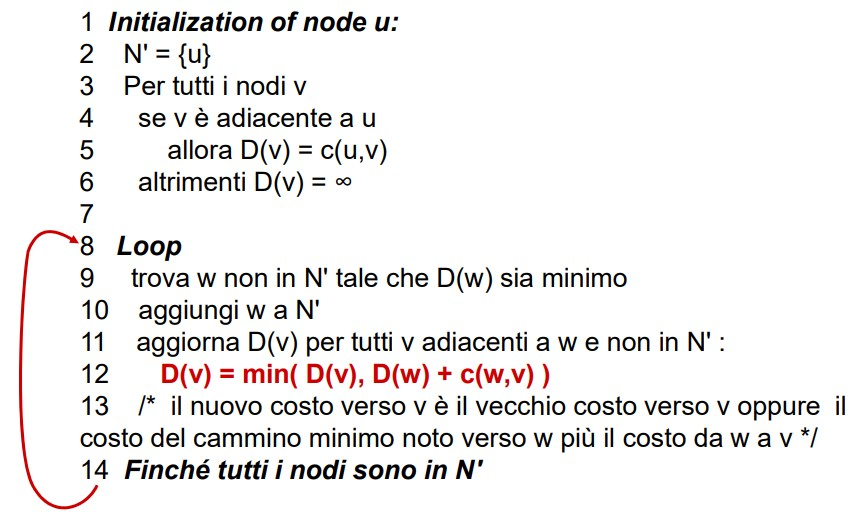
\includegraphics[width=0.7\textwidth]{immagini/Dijkstra.jpg}
    \caption*{Algoritmo di Dijkstra}
\end{figure}

\subsubsection{Link-state vs Distance vector}

\begin{table}[H]
    \centering
    \begin{tabular}{m{15em}|m{15em}}
        \textbf{\emph{Link-state}} & \textbf{\emph{Distance vector}}                                                                                          \\
        \hline
        \multicolumn{2}{c}{\emph{Complessità dei messaggi}}                                                                                                   \\
        \hline
        Con n nodi, E collegamenti, implica l’invio di O(nE) messaggi.\
                                   & Richiede scambi tra nodi adiacenti.\
        Il tempo di convergenza può variare.\
        \\
        \hline
        \multicolumn{2}{c}{\emph{Velocità di convergenza}}                                                                                                    \\
        \hline
        O(n\textsuperscript{2}).\
                                   & Può convergere lentamente, può presentare cicli d’instradamento, può presentare il problema del conteggio all’infinito.\
        \\
        \hline
        \multicolumn{2}{c}{\emph{Robustezza}}                                                                                                                 \\
        \hline
        Un router può comunicare via broadcast un costo sbagliato per uno dei suoi collegamenti connessi (ma non per altri).\
        I nodi si occupano di calcolare soltanto le proprie tabelle.\
                                   & Un nodo può comunicare cammini a costo minimo errati a tutte le destinazioni.\
        La tabella di ciascun nodo può essere usata degli altri.\
        Un calcolo errato si può diffondere per l’intera rete.                                                                                                \\
        \hline
    \end{tabular}
\end{table}

\subsection{Protocolli di routing unicast}

\subsubsection{\emph{Struttura di Internet}}

Prima di parlare dei protocolli di routing unicast dobbiamo comprendere la struttura attuale di Internet.\
La rete è cambiata, passando da una topologia ad albero, con un'unica dorsale (backbone), a una topologia con dorsali multiple gestite da aziende private.\
Anche se è piuttosto difficile offrire una visione realistica e generale di Internet oggi, possiamo dire che la sua struttura assomiglia a quanto mostrato nella Figura \ref{Struttura}.

\begin{figure}[H]
    \centering
    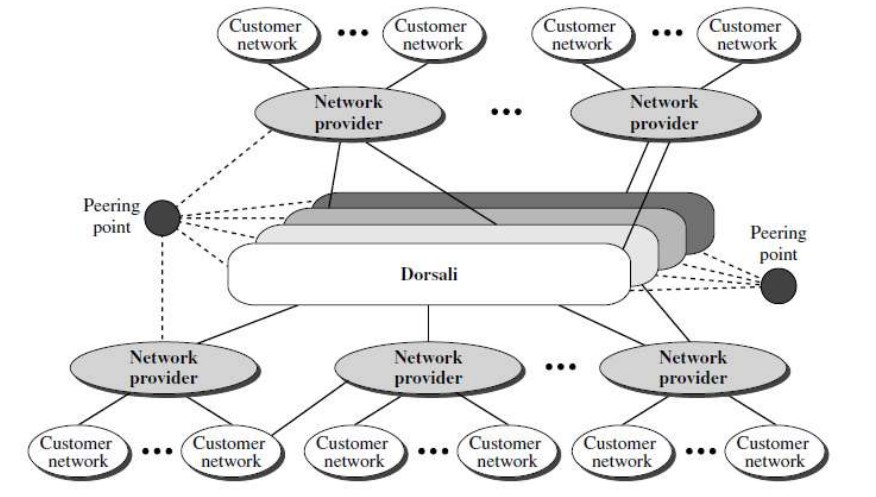
\includegraphics[width=0.8\textwidth]{immagini/Struttura_Internet.jpg}
    \caption{Struttura di Internet}
    \label{Struttura}
\end{figure}
Ci sono numerosi dorsali, gestite da società private di telecomunicazioni, che forniscono la connettività globale.\
Tali dorsali sono connesse tramite alcuni \emph{peering point} che consentono la connettività tra dorsali.\
A livello inferiore, ci sono dei network provider (fornitori di rete) che utilizzano le dorsali per avere connettività globale ma principalmente forniscono servizi di connettività a clienti Internet.\
Infine ci sono le customer network (reti dei clienti) che usano i servizi forniti dai network provider.\
Tutte queste attività (dorsali, network provider o customer network) possono essere definite Internet Service Provider (ISP).\
In tutti e tre i casi forniscono dei servizi, ma a livelli differenti.

\paragraph{\emph{Routing gerarchico}}

Internet oggi è costituita da un numero enorme di reti e di router che le collegano.\
È ovvio che il routing su Internet non può essere effettuato usando un singolo protocollo, per due ragioni:\ un problema di scalabilità e un problema amministrativo.\
Il \emph{problema di scalabilità} è dato dalla dimensione delle tabelle d'inoltro:\ sono enormi.\
Quindi, la ricerca di una destinazione in una di queste tabelle farebbe perdere molto tempo e gli aggiornamenti creerebbero una gigantesca quantità di traffico.\
Il \emph{problema amministrativo} è dato dalla struttura di Internet.\
Come mostra la Figura \ref{Struttura}, ogni ISP è un'autorità amministrativa autonoma.\
L'amministratore deve (e vuole) avere il controllo sul suo sistema.\
La società proprietaria dell'ISP deve poter utilizzare tutte le sottoreti ed i router di cui ha bisogno, deve poter scegliere di usare router di uno specifico produttore, di voler eseguire un particolare algoritmo di routing che risponde alle esigenze dell'azienda e deve poter imporre una politica specifica sul traffico che passa attraverso l'ISP.

Implementare un routing gerarchico significa considerare ogni ISP come un \emph{sistema autonomo (Autonomous System, AS)}.\
Ogni AS può eseguire un protocollo di routing che soddisfa le sue esigenze.\
A livello di Internet globale, questo non è possibile:\ è necessario un protocollo di routing globale in grado di unire assieme tutti gli AS.\
Il protocollo di routing usato all'interno degli AS viene definito \emph{protocollo di routing intra-AS}, \emph{protocollo di routing intra-dominio} \emph{(interdomain routing protocol)}, o \emph{Interior Gateway Protocol} (\emph{IGP}); il protocollo di routing globale viene definito \emph{protocollo di routing inter-AS}, \emph{protocollo di routing inter-dominio} (\emph{interdomain routing protocol}) o \emph{Exterior Gateway Protocol} (\emph{EGP}).\
Ci sono numerosi protocolli di routing intra-dominio, e ogni AS è libero di sceglierne uno, ma dovrebbe essere chiaro che dobbiamo avere un solo protocollo inter-dominio che gestisce il routing tra queste entità.\
Attualmente i due protocolli di routing intra-dominio più comuni sono RIP e OSPF; l'unico protocollo di routing inter-dominio è il BGP.

\paragraph{\emph{I sistemi autonomi}}

Come si è detto in precedenza, ogni ISP è un sistema autonomo quando si tratta di gestire le reti ed i router sotto il suo controllo.\
Anche se possono esserci AS piccoli, di medie dimensioni e grandi, ad ogni AS viene assegnato un numero identificativo (autonomous number, ASN) dall'ICANN.\
L'ASN è un numero intero senza segno, di 16 bit, che identifica in modo univoco l'AS.\
I sistemi autonomi, tuttavia, non sono classificati rispetto alla loro dimensione; vengono classificati a secondo del modo in cui sono connessi agli altri AS.\
Abbiamo degli AS stub (terminali), degli AS multihomed (a collegamenti multipli) e degli AS di transito.\
Il tipo influenza il funzionamento del protocollo di routing inter-dominio rispetto all'AS.

\begin{itemize}
    \item \textbf{\emph{AS stub}}.\
          Un AS stub ha un solo collegamento verso un altro AS.\
          Il traffico dati può essere generato da o destinato ad un AS stub ma non può accadere che i dati transitino attraverso l'AS.\
          Un buon esempio di AS stub è la rete di una grande azienda che può essere solamente sorgente o destinazione dei dati.
    \item \textbf{\emph{AS multihomed}}.\
          Un AS multihomed ha più di una connessione con altri AS, ma non consente al traffico dei dati di passare attraverso di esso.\
          Un buon esempio di questo tipo di AS è quello di un'azienda che può usare i servizi di più di un network provider ma come politica impone che gli AS a cui è collegata non possano sfruttare la sua rete per il transito dei loro dati.
    \item \textbf{\emph{AS di transito}}.\
          Un AS di transito è collegato a vari AS e consente anche il transito del traffico dati.\
          I network provider e le dorsali sono dei buoni esempi di AS di trasito.
\end{itemize}

\subsubsection{\emph{Routing Information Protocol (RIP)}}

Il \emph{Routing Information Protocol (RIP)} è uno dei protocolli di routing intra-dominio più ampiamente usati ed è basato sull'algoritmo di instradamento a vettore distanza che abbiamo descritto in precedenza.

\paragraph{\emph{Conto dei salti (hop)}}

In RIP, ogni router a grandi linee implementa l'algoritmo a vettore distanza.\
Tuttavia, l'algoritmo è stato modificato come descritto in seguito.\
Per prima cosa, siccome un router in un AS deve sapere come inoltrare un pacchetto alle diverse sottoreti presenti nell'AS, i router RIP rendono noto il costo per raggiungere le diverse sottoreti invece dei costi per raggiungere i nodi del grafo.\
In altre parole, il costo viene definito tra un router e la rete nella quale si trova l'host di destinazione.\
Secondo, la gestione dei costi viene gestita in modo molto semplice ed indipendentemente da fattori quali le prestazioni dei router e dei collegamenti, come ad esempio:\ ritardi, ampiezza della banda, ecc.\
Quindi, il costo viene definito come il numero di salti (hop), cioè il numero di sottoreti, che un pacchetto deve visitare per andare dal router sorgente all'host di destinazione.\
Da notare che la rete nel quale si trova l'host sorgente non viene considerata in questo calcolo.\
Questo perché l'host sorgente non usa alcuna tabella d'inoltro:\ il pacchetto viene semplicemente consegnato al router di default.\
La Figura \ref{RIP} mostra un esempio di quanto descritto finora.\
In RIP il costo massimo di un percorso è di 15 hop, il che significa che il valore 16 rappresenta l'infinito (nessuna connessione).\
Per tale ragione è possibile usare RIP in sistemi autonomi nei quali il diametro dell'AS non supera i 15 hop.

\begin{figure}[H]
    \centering
    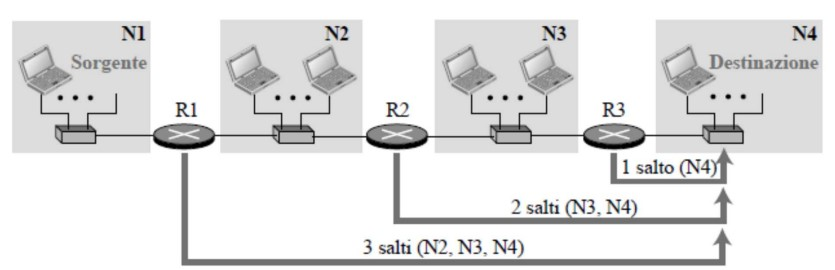
\includegraphics[width=\textwidth]{immagini/RIP.jpg}
    \caption{Conto degli hop in RIP}
    \label{RIP}
\end{figure}

\paragraph{\emph{Tabelle d'inoltro}}

L'algoritmo a vettore distanza di cui abbiamo parlato nella sezione precedente ha lo scopo principale di scambiare vettori distanza tra nodi vicini.\
Invece, nel caso dei router di un AS il loro obiettivo è quello di costruire delle tabelle d'inoltro per far giungere i pacchetti alla loro rete di destinazione.

In RIP, una tabella d'inoltro è formata da tre colonne:\ nella prima c'è l'indirizzo della rete di destinazione, nella seconda l'indirizzo del prossimo router al quale il pacchetto deve essere inoltrato e nella terza il costo (numero di hop) per raggiungere la rete di destinazione.\
La Figura \ref{Tabelle} mostra le tre tabelle d'inoltro per i router della Figura \ref{RIP}.\
Si noti che la prima e la terza colonna insieme contengono le stesse informazioni di un vettore distanza, ma con la differenza che in questo caso il costo mostra il numero di salti fino alla rete di destinazione.

\begin{figure}[H]
    \centering
    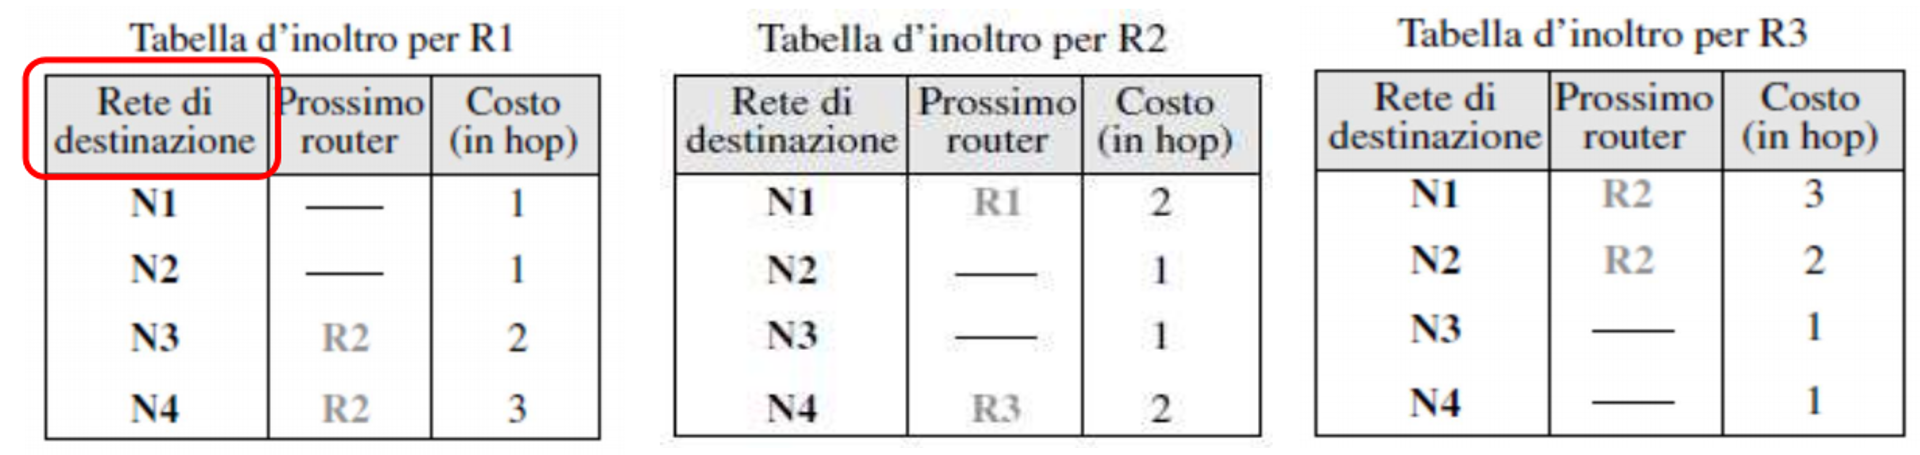
\includegraphics[width=\textwidth]{immagini/Tabelle_inoltro_RIP.png}
    \caption{Tabelle d'inoltro}
    \label{Tabelle}
\end{figure}

Anche se una tabella d'inoltro RIP definisce solo il prossimo router (nella seconda colonna), questa informazione è sufficiente per ricostruire l'intero albero minimo.\
Ad esempio R1 definisce che il prossimo router per il percorso verso N4 è R2; R2 definisce che il prossimo router per N4 è R3; R3 definisce che non c'è alcun router successivo per tale percorso.\
Quindi l'albero è R1$\rightarrow$R2$\rightarrow$R3$\rightarrow$N4.

Ci si potrebbe chiedere qual è l'uso della terza colonna della tabella d'inoltro.\
La terza colonna non è necessaria per inoltrare il pacchetto, ma serve per aggiornare la tabella d'inoltro quando ci sono modifiche del percorso.

\paragraph{\emph{Implementazione di RIP}}

Il RIP è implementato per mezzo di un processo demone (sempre attivo) che ascolta sulla porta nota 520 UDP.\
Nel caso di UNIX BSD tale processo viene chiamato \textbf{routed} (come abbreviazione di route daemon).\
Questo significa che anche se RIP è un protocollo di routing, usato per consentire a IP di instradare i datagrammi attraverso gli AS, i messaggi RIP vengono incapsulati all'interno di datagrammi utente UDP, che a loro volta sono incapsulati in datagrammi IP.\
In altre parole, RIP lavora a livello di applicazione ma crea delle tabelle d'inoltro per IP (che si trova a livello di rete).\

Gli aggiornamenti vengono inviati ogni 30 secondi (circa) o se la tabella d'inoltro cambia.

\paragraph{\emph{Algoritmo RIP}}

Il RIP implementa l'algoritmo d'instradamento a vettore distanza di cui abbiamo parlato nella sezione precedente.\
Tuttavia sono necessari alcuni cambiamenti all'algoritmo per permettere a un router di aggiornare la sua tabella d'inoltro:
\begin{itemize}
    \item Invece di inviare solamente vettori distanza, un router deve inviare l'intero contenuto della sua tabella d'inoltro all'interno di un aggiornamento.
    \item Il destinatario aggiunge un hop a ciascun costo e modifica il campo ``router successivo'' inserendo l'indirizzo del router mittente.\
          Ogni percorso nella tabella d'inoltro modificata viene definito \emph{percorso ricevuto} e ogni percorso nella vecchia tabella d'inoltro viene chiamato \emph{vecchio percorso}.\
          Il router ricevente seleziona i vecchi percorsi come nuovi ad eccezione dei seguenti tre casi:
          \begin{enumerate}
              \item se il percorso ricevuto non esiste nella vecchia tabella d'inoltro allora va aggiunto;
              \item se il costo del percorso ricevuto è inferiore al costo di quello vecchio, il percorso ricevuto va selezionato come nuovo percorso;
              \item se il costo del percorso ricevuto è maggiore rispetto a quello del vecchio percorso, ma il valore del prossimo router è lo stesso in entrambi i percorsi, allora il percorso ricevuto va selezionato come nuovo.\
                    Questo è il caso in cui il percorso era stato reso noto dallo stesso router in passato, ma ora la situazione è cambiata.
          \end{enumerate}
    \item La nuova tabella d'inoltro deve essere ordinata in base al percorso di destinazione (in ordine di lunghezza del prefisso).
\end{itemize}

\subsubsection{\emph{Open Shortest Path First (OSPF)}}

L'\emph{Open Shortest Path First} è anch'esso un protocollo di routing intra-dominio come il RIP, ma si basa sull'instradamento a stato del collegamento che abbiamo descritto in precedenza.\
L'OSPF è un protocollo \emph{aperto}, il che significa che la sua specifica è un documento pubblico.

\paragraph{\emph{Metrica}}

Nell'OSPF, come nel RIP, il costo per raggiungere una destinazione dall'host si calcola dal router sorgente alla rete di destinazione.\
Tuttavia, ad ogni collegamento (rete attraversata) può venire assegnato un peso a seconda del suo throughput, tempo di round-trip, affidabilità, ecc.\
Un amministratore, eventualmente, può anche decidere di usare come metrica il numero di hop.\
La Figura \ref{fig:OSPF} dà l'idea del computo del costo da un router fino alla rete dell'host di destinazione.\
Possiamo confrontare questa figura con quella relativa al RIP (Figura \ref{RIP}).

\begin{figure}[H]
    \centering
    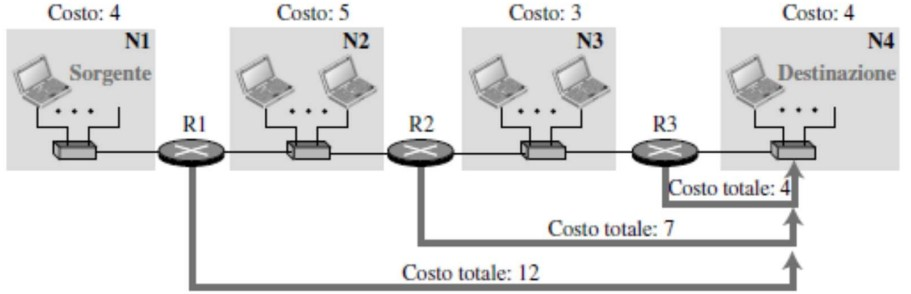
\includegraphics[width=\textwidth]{immagini/OSPF.jpg}
    \caption{Utilizzo dei costi come metrica in OSPF}
    \label{fig:OSPF}
\end{figure}

\paragraph{\textbf{Tabelle d'inoltro}}

Ogni router OSPF crea una tabella d'inoltro dopo aver trovato l'albero a percorso minimo tra se stesso e la destinazione usando l'algoritmo di Dijkstra.\
La Figura \ref{fig:Tabella_OSPF} mostra una tabella d'inoltro per il semplice AS della Figura \ref{fig:OSPF}.
\begin{figure}[H]
    \centering
    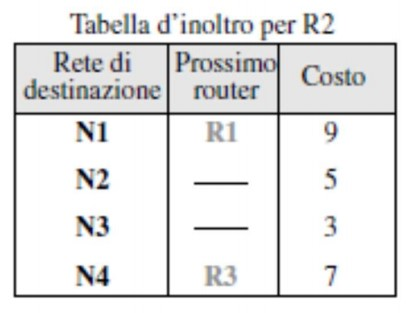
\includegraphics[width=0.3\textwidth]{immagini/Tabelle_inoltro_OSPF.jpg}
    \caption{Tabella d'inoltro dell'OSPF}
    \label{fig:Tabella_OSPF}
\end{figure}
Confrontando le tabelle d'inoltro per l'OSPF e il RIP nello stesso AS, troviamo che l'unica differenza sono i valori di costo.\
In altre parole se usiamo il conteggio dei salti per l'OSPF allora le tabelle saranno esattamente identiche.\
Il motivo è che entrambi i protocolli usano gli alberi a percorso minimo per definire il percorso migliore da una sorgente alla destinazione.

\paragraph{\emph{Aree}}

Rispetto al RIP, che normalmente viene usato in AS piuttosto piccoli, l'OSPF è stato progettato per poter gestire il routing in AS di tutte le dimensioni.\
Tuttavia, la costruzione degli alberi a percorso minimo nell'OSPF richiede che tutti i router inondino (flooding) l'intero AS con i loro LSP per creare LSDB globale.\
In altre parole, tutti i router devono inviare il loro LSP a tutti gli altri router dell'AS.\
Anche se ciò non è un problema negli AS piccoli, potrebbe creare un enorme volume di traffico in AS di medie o grandi dimensioni.\
Per evitare ciò, l'AS può essere diviso in settori più piccoli chiamati \emph{aree}.\
Ogni area è un piccolo dominio indipendente per il flooding degli LSP.\
In pratica l'OSPF usa un altro livello di gerarchia nel routing:\ il primo è il sistema autonomo e il secondo è l'area al suo interno.

Tuttavia, ogni router che si trova in un'area ha bisogno di conoscere lo stato dei collegamenti non solo dell'area ma anche delle altre.\
Per tale ragione una delle aree dell'AS viene definita \emph{area dorsale (backbone area)}, il cui compito è proprio quello di collegare tra loro le varie aree.\
I router nell'area dorsale hanno la responsabilità di raccogliere le informazioni delle varie aree e comunicarle.\
In questo modo un router che si trova in un'area può ricevere tutti gli LSP generati nelle altre aree.\
Per implementare la comunicazione, ogni area è contraddistinta da un identificatore, e l'identificatore della dorsale è lo zero.\
La Figura \ref{fig:AS} illustra un AS e le sue aree.

\begin{figure}[H]
    \centering
    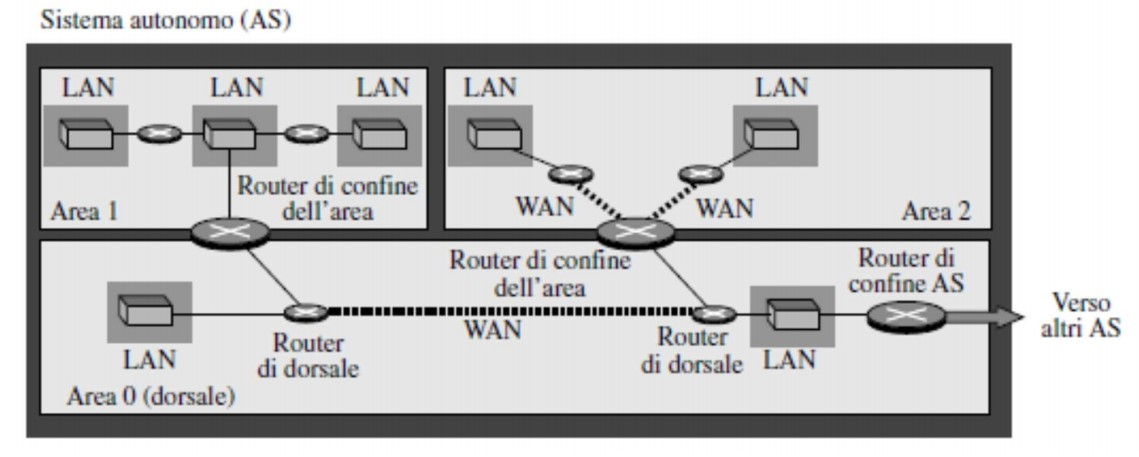
\includegraphics[width=0.7\textwidth]{immagini/AS.jpg}
    \caption{Caption}
    \label{fig:AS}
\end{figure}

\paragraph{\emph{Implementazione dell'OSPF}}

L'OSPF è implementato come applicazione che sfrutta la comunicazione a livello di rete usando direttamente il protocollo IP.\
I datagrammi IP che incapsulano un messaggio OSPF hanno il valore del campo protocollo impostato a 89.\
Questo significa che, anche se OSPF è un protocollo di routing usato per permettere l'instradamento dei datagrammi all'interno di un AS, esso stesso è incapsulato direttamente all'interno di datagrammi IP.

\subsubsection{Sistemi autonomi interconnessi}

Ogni AS nella figura usa uno dei due protocolli d'instradamento intra-domi\-nio che abbiamo visto (RIP o l'OSPF).\
Ogni router all'interno degli AS sa come raggiungere tutte le reti che si trovano nel suo AS, ma non sa come raggiungere una rete che si trova in un altro AS.\
Per fare ciò viene usato il protocollo BGP4, l'\textbf{unico} protocollo INTER-AS usato in Internet, che permette a coppie di router di scambiarsi informazioni su connessioni TCP.
\begin{figure}[H]
    \centering
    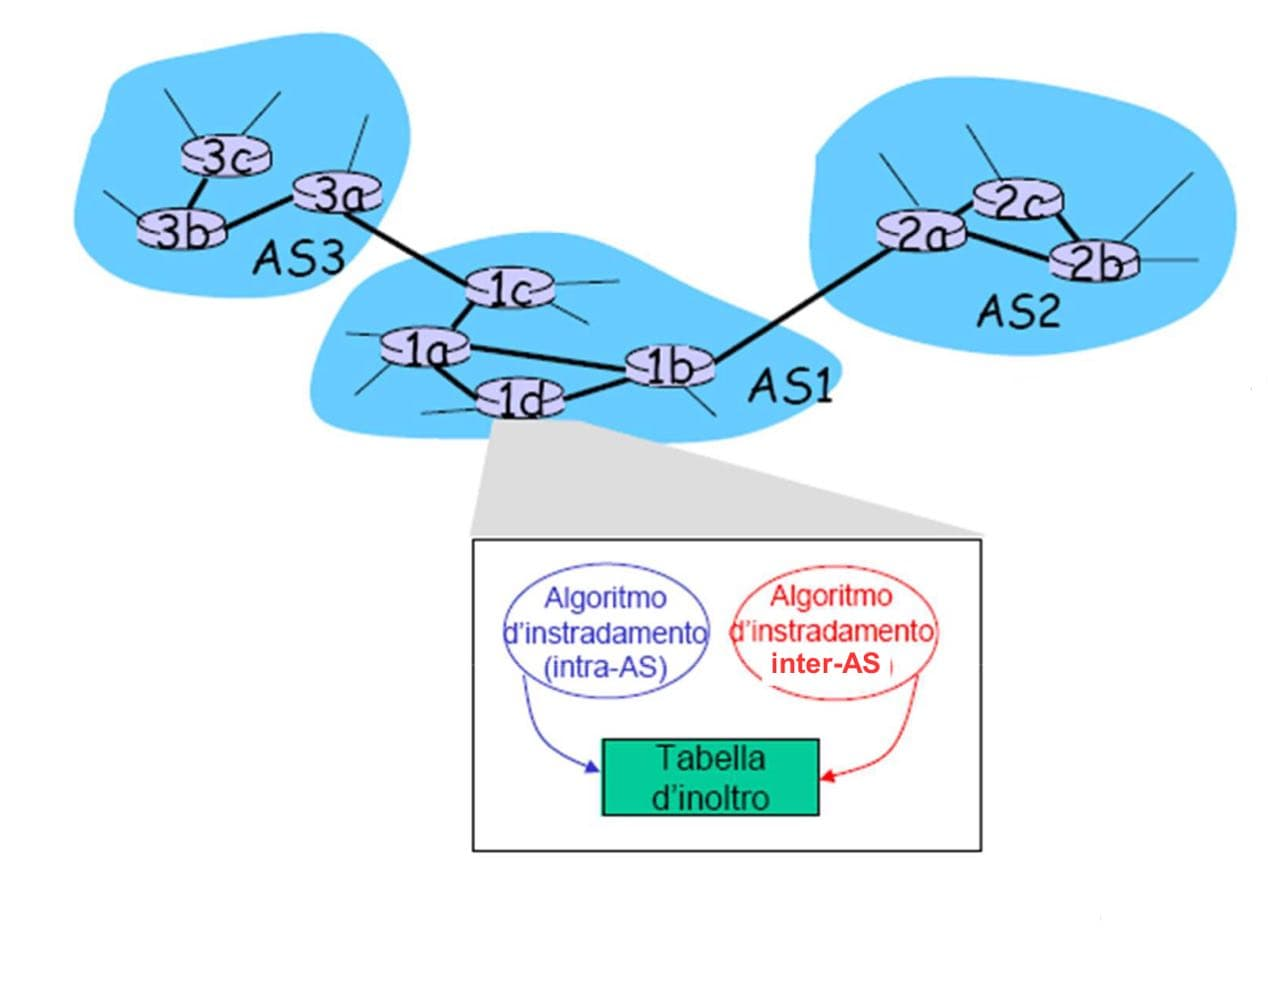
\includegraphics[width=0.6\textwidth]{immagini/AS_interconnessi.jpg}
    \caption*{Sistemi autonomi interconnessi}
\end{figure}
\begin{figure}[H]
    \centering
    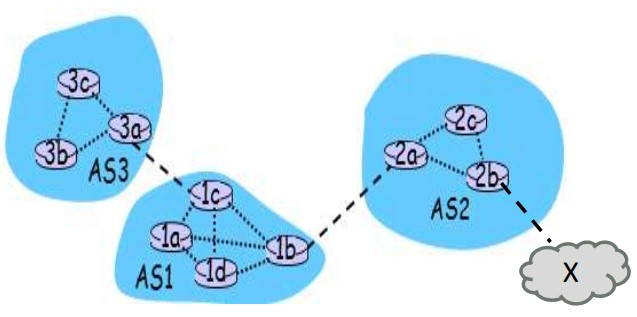
\includegraphics[width=0.5\textwidth]{immagini/AS_interconnessi_esempio.jpg}
    \captionsetup{singlelinecheck=off}
    \caption*{\footnotesize
        \begin{itemize}
            \item AS1 scopre (grazie a INTER-AS routing protocol) che una sottorete X è raggiungibile via AS2 (a cui AS1 è collegato mediante il gateway 1b)
            \item AS1 propaga (con INTER-AS routing protocol) tale informazione al suo interno
            \item Un router R (es.\ 1d in figura) di AS1 riceve l’informazione ``rete X raggiungibile via AS2'' e aggiorna (se necessario) la tabella di inoltro
        \end{itemize}
    }
\end{figure}

Per permettere ad ogni router di instradare correttamente i pacchetti, qualsiasi sia la destinazione, è necessario installare su tutti i router di confine (border router) dell'AS una variante del BGP chiamata \emph{BGP esterno} (\emph{external BGP, eBGP}).\
Tutti i router (non solamente quelli di confine) dovranno invece usare la seconda variante del BGP, chiamata \emph{BGP interno} (\emph{internal BGP, iBGP}).\
Questo significa che i router di confine devono eseguire ben tre protocolli d'instradamento (intra-dominio, eBGP e iBGP) e che tutti gli altri router ne eseguono due (intra-dominio e iBGP).
\begin{itemize}
    \item Aggregazione indirizzi:\ destinazioni rappresentate da prefissi CIDR
    \item Pubblicizzare un prefisso significa impegnarsi a instradare pacchetti destinati a reti in quel prefisso
    \item Distribuzione di informazioni su raggiungibilità:\ un gateway riceve informazioni da gateway di altri AS su sessione eBGP e distribuisce informazioni ai router interni della propria rete su sessioni iBGP.\
          Altri gateway dell’AS possono ri-pubblicizzare info con eBGP.
    \item Advertisement (ADV) BGP:\ ``route'' = prefisso + attributi.\
          I due attributi più importanti sono
          \begin{itemize}
              \item AS\_PATH:\ sequenza degli AS attraversati nel path pubblicizzato dall’advertisement.\
                    Usato per scartare advertisement già ricevuti e scegliere tra più percorsi per lo stesso prefisso
              \item NEXT\_HOP:\ indica l'indirizzo IP del primo router lungo un percorso annunciato (al di fuori dell'AS che riceve l'annuncio) a un dato prefisso di rete
          \end{itemize}
    \item Politiche di importazione:\ quando un gateway riceve un ADV, usa tali politiche per accettare/rifiutare ADV
    \item Scelta delle rotte:\ un router può ricevere più di una rotta per lo stesso prefisso.\
          Sequenza di regole (principale):
          \begin{enumerate}
              \item Attributo di ``preferenza locale'' (LOCAL-PREF scelta da amministratore o impostato dai router dell’AS) $\rightarrow$ vengono selezionati quelli coi valori più alti
              \item Shortest AS-PATH
              \item Closest NEXT-HOP interface (``hot potato routing'')
          \end{enumerate}
\end{itemize}

\section{IP versione 6}

Nell'ultima parte di questo capitolo, si parlerà del protocollo IP di nuova generazione:\ IPv6.\
L'esaurimento degli indirizzi e alcune limitazioni di IPv4, già nei primi anni '90, hanno portato allo sviluppo di una nuova versione del protocollo.\
Questa nuova versione, chiamata \emph{Internet Protocol versione 6} (IPv6) o \emph{IP di nuova generazione} (\emph{IP new generation}, \emph{IPng}) è nata con lo scopo di aumentare lo spazio degli indirizzi rispetto a IPv4, ridisegnare il formato dei datagrammi IP e allo stesso tempo rivedere anche alcuni protocolli ausiliari come ICMP.\
È interessante sapere che IPv5 era una proposta basata sul modello OSI ma non si è mai concretizzata.\
Quanto segue mostra i principali cambiamenti nel protocollo IPv6.

\begin{itemize}
    \item \textbf{\emph{Spazio degli indirizzi di dimensione maggiore}}.\
          Un indirizzo IPv6 è lungo 128 bit.\
          Paragonato ai 32 bit dell'IPv4, è un enorme aumento (2\textsuperscript{96} volte) dello spazio degli indirizzi.
    \item \textbf{\emph{Miglior formato dell'intestazione}}.\
          IPv6 utilizza un nuovo formato per l'intestazione (header) dei datagrammi.\
          Nell'intestazione IPv6 le opzioni sono separate dall'intestazione di base e inserite, quando necessario, tra l'intestazione di base e i dati.\
          Ciò semplifica e velocizza il processo di routing visto che la maggior parte delle opzioni non è necessario che sia controllata dai router.
    \item \textbf{\emph{Nuove opzioni}}.\
          IPv6 supporta nuove opzioni per consentire l'implementazione di funzionalità aggiuntive.
    \item \textbf{\emph{Possibilità di estensione}}.\
          L'IPv6 è progettato per consentire l'estensione del protocollo se richiesto dall'introduzione di nuovo tecnologie o applicazioni.
    \item \textbf{\emph{Supporto per l'allocazione delle risorse}}.\
          In IPv6 è stato rimosso il campo tipo del servizio (Type Of Service, TOS) che è presente in IPv4.\
          Al suo posto sono stati aggiunti due nuovi campi, classe di traffico ed etichetta di flusso, per consentire alla sorgente di richiedere un trattamento speciale per il datagramma.\
          Il meccanismo, se fosse supportato dai router, potrebbe migliorare la gestione del traffico audio o video in tempo reale.
    \item \textbf{\emph{Maggiore sicurezza}}.\
          Le opzioni relative alla crittografia ed autenticazione permettono di migliorare la riservatezza e verificare l'integrità dei datagrammi.
\end{itemize}
L'adozione di IPv6 è stata lenta.\
Il motivo principale che ha portato al suo sviluppo, cioè il progressivo esaurimento degli indirizzi di IPv4, è stato rallentato grazie a tre rimedi a breve termine:\ l'indirizzamento senza classi, l'uso del protocollo DHCP e soprattutto la diffusione del NAT.\
Il fatto che si tratti di soluzioni a breve termine, che non risolvono a fondo il problema, e l'uso sempre più ampio di nuovi servizi (per esempio, l'uso del protocollo IP in mobilità, la telefonia basata su IP ecc.) prima o poi richiederanno la sostituzione totale di IPv4 con IPv6.\
In passato si prevedeva che questa migrazione sarebbe avvenuta entro il 2010, cosa che in effetti non è successa.\
Le previsioni attuali parlano invece del 2020, ma probabilmente si andrà ben oltre.

\subsection{Formato dei datagrammi IPv6}

Il formato dei datagrammi IPv6 è mostrato nella Figura \ref{fig:IPv6}.\
Ciascun datagramma è composto da un'intestazione di base (base header) seguita dai dati (payload).\
L'intestazione di base occupa 40 byte, mentre il payload può arrivare fino a 65.535 byte.\
Segue la descrizione dei diversi campi.
\begin{figure}[H]
    \centering
    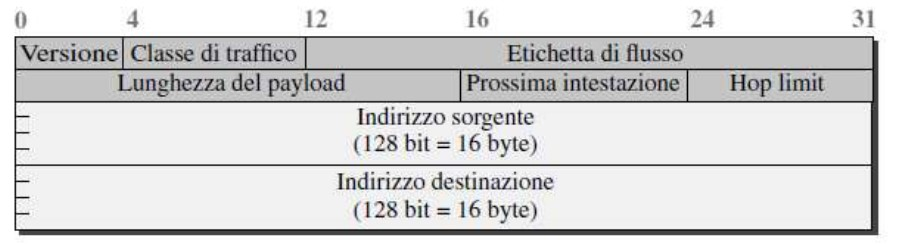
\includegraphics[width=0.7\textwidth]{immagini/IPv6.jpg}
    \caption{Formato dei datagrammi IPv6}
    \label{fig:IPv6}
\end{figure}

\begin{itemize}
    \item \textbf{\emph{Versione} (\emph{version})}.\
          Il campo versione (4 bit) definisce il numero di versione del protocollo IP.\
          Per l'IPv6, il valore è 6.
    \item \textbf{\emph{Classe di traffico} (\emph{traffic class})}.\
          Il campo classe di traffico (8 bit) è utilizzato per distinguere il tipo di servizio di trasferimento a seconda della tipologia di dati contenuti nel payload.\
          Esso sostituisce il campo \emph{tipo di servizio} (Type Of Service, TOS) che è presente in IPv4.
    \item \textbf{\emph{Etichetta di flusso} (\emph{flow label})}.\
          L'etichetta di flusso (20 bit) dovrebbe permettere una nuova gestione dei dati sotto forma di flusso di datagrammi, rispetto ai singoli datagrammi indipendenti come accade in IPv4.
    \item \textbf{\emph{Lunghezza del payload} (\emph{payload length})}.\
          Il campo lunghezza del payload (2 byte) definisce la lunghezza del datagramma IP escludendo l'intestazione.\
          Si noti che in IPv4 ci sono due campi legati dalla lunghezza:\ lunghezza dell'intestazione e lunghezza totale.\
          Invece in IPv6, la lunghezza dell'intestazione di base è fissa (40 byte), quindi è necessario indicare solamente la lunghezza del payload.
    \item \textbf{\emph{Prossima intestazione} (\emph{next header})}.\
          La prossima intestazione è un campo (8 bit) che definisce il tipo della prima intestazione estesa (extension header), se presente, o il tipo dei dati che seguono l'intestazione di base all'interno del payload.\
          Questo campo è simile al campo ``protocollo'' che è presente in IPv4.
    \item \textbf{\emph{Hop limit} (\emph{numero massimo di salti})}.\
          Il campo hop limit ha la stessa funzione del campo TTL in IPv4.
    \item \textbf{\emph{Indirizzo sorgente e indirizzo destinazione} (\emph{source and destination address})}.\
          I campi indirizzo sorgente e destinazione sono indirizzi Internet da 16 byte (128 bit) che identificano la sorgente originale del datagramma e la sua destinazione.
    \item \textbf{\emph{Dati} (\emph{payload})}.\
          Se confrontato con IPv4, il campo payload in IPv6 ha una forma e un significato differenti.
\end{itemize}
Il campo dati in IPv6 può contenere una combinazione di zero o più intestazioni estese (usate per rappresentare le varie opzioni) seguite dai dati provenienti da altri protocolli (UDP, TCP e così via).\
In IPv6, le opzioni, che fanno parte dell'intestazione in IPv4, sono implementate sotto forma di intestazioni estese.\
Il campo dati può contenere tante intestazioni quante ne sono necessarie.\
Ogni intestazione è formata da due campi obbligatori, intestazione successiva (next header) e lunghezza (lenght), seguite dalle informazioni specifiche delle varie opzioni.\
Si noti l'uso che viene fatto del campo ``prossima intestazione'' (next header):\ definisce il tipo della prossima intestazione quando si riferisce a un'opzione oppure identifica il protocollo incapsulato nel payload del datagramma.

\subsubsection{\emph{Concetto di flusso e priorità in IPv6}}

Il protocollo IP era inizialmente progettato come protocollo senza connessione.\
Tuttavia, soprattutto a causa di alcune tecnologie di livello inferiore, c'è una certa tendenza ad usare IP come protocollo orientato alla connessione.\
Per questo motivo, nella versione 6 è stata aggiunta un'etichetta di flusso nell'intestazione che permette questa forma di utilizzo.\
Ovviamente questo è possibile solamente quando i router offrono il supporto per questa modalità particolare di gestione dei datagrammi.

In un router, un flusso non è altro che una sequenza di datagrammi che hanno le stesse caratteristiche (come ad esempio il percorso, l'uso delle stesse risorse, gli stessi requisiti di sicurezza ecc.).\
Un router che supporta la gestione delle etichette di flusso possiede una tabella delle etichette di flusso.\
Questa tabella ha una voce per ogni etichetta di flusso attiva, ognuna di queste voci identifica i requisiti di servizio richiesti dal quel particolare flusso.\
In questo modo, quando un router riceve un datagramma, consulta la tabella delle etichette di flusso per trovare la voce corrispondente al flusso indicato nell'intestazione del datagramma ed identifica quindi i suoi requisiti.\
Ovviamente l'etichetta di flusso indicata nel datagramma non specifica direttamente quali sono questi requisiti; queste informazioni dovranno essere propagate ai router per mezzo di altre modalità come ad esempio l'uso di opzioni oppure altri protocolli.

Nella sua forma più semplice un'etichetta di flusso può essere utilizzata per accelerare l'elaborazione dei datagrammi da parte del router.\
Quando un router riceve un datagramma, invece di consultare la tabella d'inoltro e dover eseguire un algoritmo d'instradamento per determinare l'indirizzo del salto successivo, può semplicemente accedere alla tabella delle etichette di flusso per trovare il salto successivo.

Nella sua forma più sofisticata, un'etichetta di flusso può essere usata per fornire un miglior supporto alla trasmissione di audio e video in tempo reale.\
Le applicazioni multimediali richiedono risorse come un'elevata ampiezza di banda, grandi buffer, potenza di calcolo e così via.\
Un'applicazione di questo tipo potrebbe riservare in anticipo le risorse di rete necessarie per garantire che i dati non siano ritardati per mancanza di risorse.

\subsubsection{\emph{Frammentazione e riassemblaggio}}

In IPv6 la frammentazione e il riassemblaggio esistono ancora ma rispetto ad IPv4 c'è una differenza fondamentale.\
I datagrammi IPv6 possono essere frammentati solo dalla sorgente e non dai router lungo il percorso.\
Ovviamente, anche in questo caso, il riassemblaggio avviene solamente alla destinazione.\
La frammentazione dei datagrammi nei router non è consentita per velocizzare l'elaborazione da parte del router; è bene ricordare che la frammentazione di un datagramma richiede un'elaborazione piuttosto complessa visto che comporta la modifica di vari campi dell'intestazione.\
In IPv6, l'host sorgente può verificare la dimensione del datagramma e verificare se frammentarlo o meno.\
Quando un router riceve un datagramma, controlla la sua dimensione e lo scarta nel caso sia maggiore rispetto a quanto consentito dalla MTU della rete in cui deve inoltrarlo.\
Inoltre, il router invierà un messaggio d'errore ICMPv6 (di tipo:\ pacchetto troppo grande) alla sorgente del datagramma per informarla dell'accaduto.

\subsection{Passaggio da IPv4 a IPv6}

Anche se è pronta una nuova versione del protocollo IP, rimane da capire come può essere fatto il passaggio dalla versione corrente a quella nuova.\
La prima soluzione che viene in mente, la più banale, è definire un giorno di passaggio nel quale tutti gli host e router smetteranno di usare IPv4 ed inizieranno ad usare solo IPv6.\
Ovviamente la transizione non può essere fatta in questo modo.\
A causa dell'enorme numero di sistemi in rete la migrazione non può avvenire improvvisamente.\
Ci sarà bisogno di una quantità di tempo considerevole prima che tutti i sistemi siano aggiornati.\
La transizione dovrà essere studiata accuratamente per evitare problemi tra il vecchio sistema e quello nuovo.\
L'IETF ha studiato tre strategie che possono essere implementate in questa fase:\ il dual stack (doppia pila di protocolli), il tunnelling e la traduzione dell'intestazione (header translation).

\subsubsection{\emph{Dual stack}}

La strategia prevede che tutti gli host, durante la transizione, abbiano una doppia pila di protocolli per la comunicazione in rete.\
In altre parole, ciascun host (o router) deve eseguire IPv4 e IPv6 simultaneamente fino a quando tutta la rete non sarà passata ad IPv6.\
Questa strategia è rappresentata in Figura \ref{fig:Dual_stack}.

\begin{figure}[H]
    \centering
    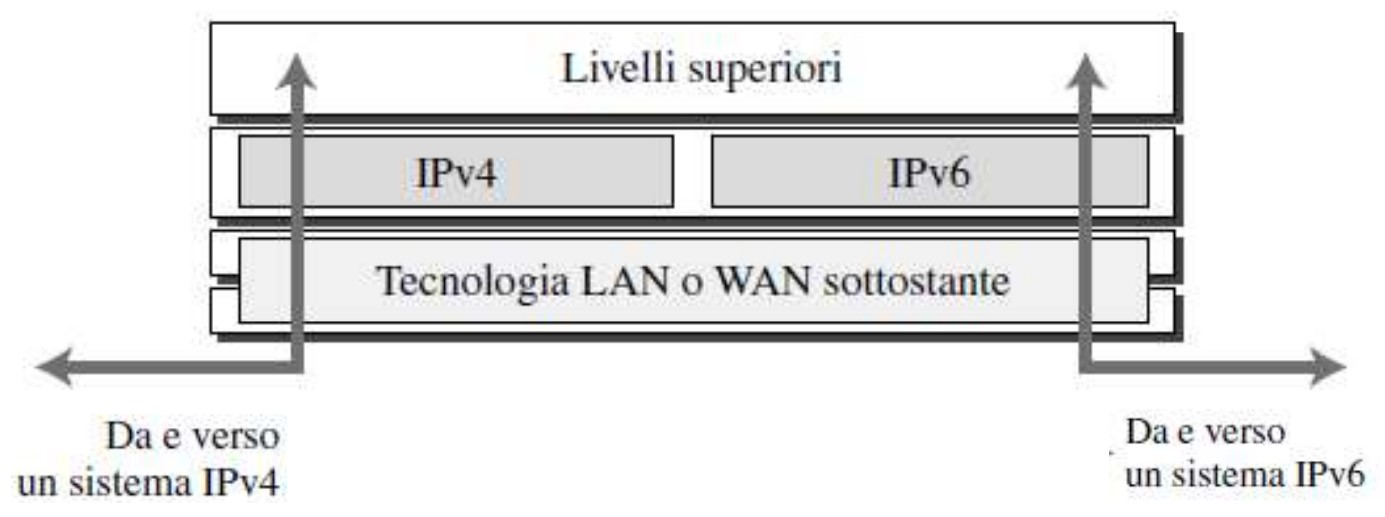
\includegraphics[width=0.6\textwidth]{immagini/Dual_stack.jpg}
    \caption{Dual stack}
    \label{fig:Dual_stack}
\end{figure}

Per determinare quale versione utilizzare quando si invia un pacchetto a una destinazione, l'host sorgente interroga il DNS.\
Se il DNS restituisce un indirizzo IPv4 allora l'host invia un pacchetto IPv4.\
Se il DNS restituisce un indirizzo IPv6 allora l'host invia un pacchettto IPv6.

\paragraph{\emph{Tunneling}}

Il tunneling è una tecnica utilizzata quando due host che usano IPv6 vogliono comunicare tra loro ma i datagrammi devono attraversare una regione della rete che usa solo IPv4.\
Per passare attraverso questa regione i datagrammi devono necessariamente avere un indirizzo IPv4.\
Una volta superata la tratta IPv4, il datagramma IPv6 potrà essere nuovamente estratto.\
È come se i datagrammi IPv6 viaggiassero all'interno di un tunnel tra due isole IPv6.\
Per rendere esplicito il fatto che il datagramma IPv4 sta trasportando un datagramma IPv6, il valore del protocollo nell'intestazione del datagramma IPv4 viene impostato a 41.

\begin{figure}[H]
    \centering
    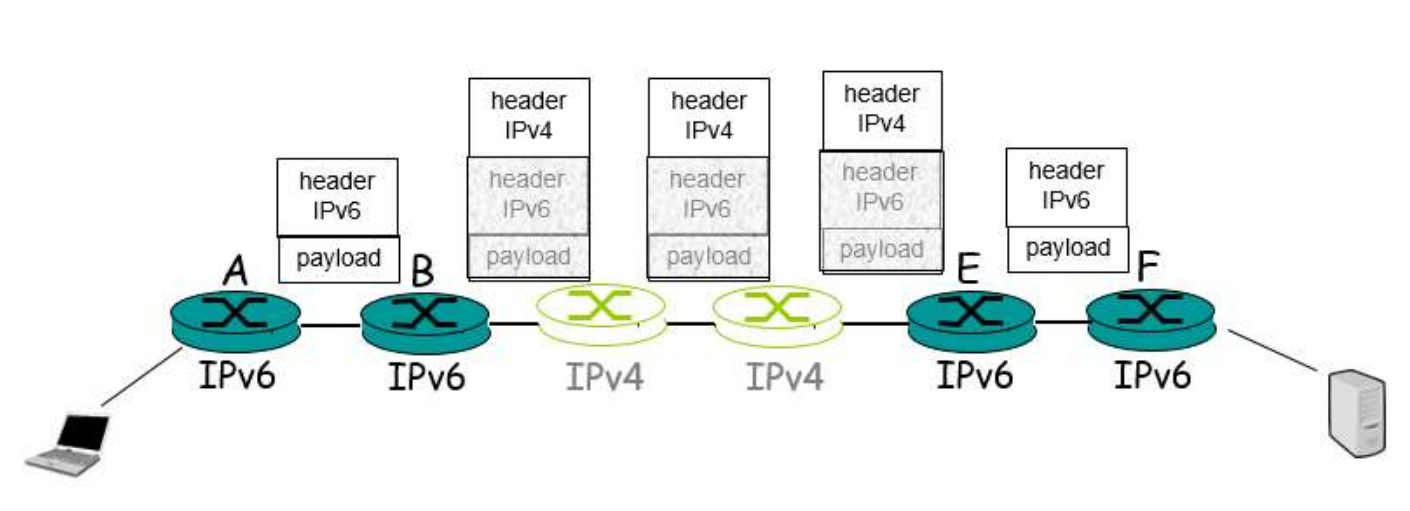
\includegraphics[width=\textwidth]{immagini/Tunneling.jpg}
    \caption*{Strategia di tunneling}
\end{figure}

\paragraph{\emph{Traduzione dell'intestazione}}

La traduzione dell'intestazione (header traslation) sarà necessaria quando la maggior parte di Internet sarà migrata ad IPv6, con alcuni sistemi residui ancora basati su IPv4.\
Supponiamo che il mittente intenda (o debba) usare IPv6, ma che il ricevente non sia in grado di supportarlo.\
In questo caso il meccanismo di tunneling non funziona.\
L'unica alternativa è quella di effettuare una traduzione completa dell'intestazione del datagramma, in modo di convertirla da IPv6 a IPv4, prima che il datagramma arrivi a destinazione.

\newpage

\section{Approfondimenti}

\subsection{Checksum}

Per quale motivo UDP e TCP si preoccupano di controllare l’integrità di informazioni di livello network se anche IP usa un suo checksum?

\begin{enumerate}
    \item Ragioni ``storiche''
    \item Checksum UDP e TCP controlla anche il payload ed è una checksum end-to-end
    \item UDP e TCP potrebbero non usare IP come servizio di rete
\end{enumerate}

\subsection{NAT:\ problemi}

\subsubsection{FTP}

\emph{Cosa succede se un client FTP sotto NAT invia RETR e il router NAT del client FTP non accetta richieste di connessioni TCP?}
\begin{figure}[H]
    \centering
    \includegraphics[width=0.7\textwidth]{immagini/FTPactive_NAT.png}
    \caption*{FTP active mode transfers through a NAT router}
\end{figure}

Poiché la connessione principale è in uscita, il firewall NAT consente di stabilire questa connessione, ma quando il server tenta di riconnettersi al client viene bloccato dal firewall.

La tecnica chiamata ``modalità passiva'' o PASV è stata introdotta per ridurre questo problema.\
In questo schema le connessioni vengono sempre effettuate dal client al server e non viceversa.

\begin{figure}[H]
    \centering
    \includegraphics[width=0.7\textwidth]{immagini/FTPpassive_NAT.png}
    \caption*{FTP passive mode transfers through a NAT router}

\end{figure}
Questo è il motivo per cui la modalità passiva è generalmente preferibile quando sono coinvolti firewall NAT.

\subsubsection{P2P}

\emph{In una applicazione P2P come può un peer chiedere di utilizzare una certa porta per poter essere contattato?}

In un'applicazione P2P, qualsiasi Peer A partecipante dovrebbe essere in grado di avviare una connessione TCP a qualsiasi altro Peer B partecipante.\
L'essenza del problema è che \textbf{se il peer B è dietro un NAT, non può agire come un server e accettare connessioni TCP}.

\begin{enumerate}
    \item Configurare staticamente il NAT per inoltrare le richieste di connessione in entrata su una determinata porta al tuo server.
    \item Protocollo Internet Gateway Device (IGD).\
          Consente all'host con NAT di aggiungere/rimuovere mappature delle porte (con tempi di lease) (ad esempio, automatizzare la configurazione statica della mappa delle porte NAT).
          \begin{figure}[H]
              \centering
              \includegraphics[width=0.4\textwidth]{immagini/IGD.png}
          \end{figure}
    \item \textbf{Connection reversal}.\
          Questo problema NAT può essere aggirato se il Peer B non è dietro un NAT.\
          In questo caso, il Peer B può prima contattare il Peer A tramite un Peer intermedio (Server S nella figura), che non è dietro un NAT e con il quale A ha stabilito una connessione TCP in corso.\
          Il peer B può quindi chiedere al peer A, tramite il server S, di avviare una connessione TCP direttamente al peer B.\
          Una volta stabilita la connessione TCP P2P diretta tra i peer A e B, i due peer possono scambiarsi messaggi o file.
          \begin{figure}[H]
              \centering
              \includegraphics[width=0.7
                  \textwidth]{immagini/Connection_reversal.png}
              \caption*{Connection reversal}
          \end{figure}
\end{enumerate}
